% \iffalse meta-comment
%                                                                
%  File: pdfx.dtx
%
%  Copyright (c) 2019, CV Radhakrishnan <cvr@river-valley.org>,
%    Han The Thanh <thanh@river-valley.org>,
%    Ross Moore <ross.moore@mq.edu.au>,
%    Peter Selinger <selinger@mathstat.dal.ca>
%                      
%  This file may be distributed and/or modified under the conditions
%  of the LaTeX Project Public License, either version 1.2 of this
%  license or (at your option) any later version.  The latest version
%  of this license is in:
%    
%    http://www.latex-project.org/lppl.txt
%    
%  and version 1.2 or later is part of all distributions of LaTeX
%  version 1999/12/01 or later.
%
% \fi
%
% \CheckSum{6309}
% \iffalse
%
%<*driver>
\pdfcompresslevel 9
\providecommand{\pdfxopt}{a-2u}
\providecommand{\lastyear}{2018}
\providecommand{\thisyear}{2019}
\begin{filecontents*}{./\jobname.xmpdata}
\Title{Generation of PDF/X- and PDF/A-compliant PDFs with pdfTeX \textemdash\ pdfx.sty}
\Author{\CVR\sep \Thanh\sep Ross Moore\sep Peter Selinger}
\Subject{This package supports generation of PDF/X-, PDF/A- and PDF/E-compliant documents, in most of their variants, using pdfLaTeX, LuaLaTeX and XeLaTeX.}
\Keywords{PDF/X-, PDF/A- and PDF/E-compliance\sep Multilingual Metadata\sep installation\sep \TeX Live \thisyear}
\PublicationType{manual}
\Contributor{Norbert Preining: 'colorprofiles' package}
\Copyright{Public domain.}
\Copyrighted{False}
\CopyrightURL{http://tug.org/texlive/}
\CoverDisplayDate{March \thisyear}
\CoverDate{\thisyear-03-10}
\CreatorTool{LaTeX + pdfx.sty with option \pdfxopt, from TeX Live \thisyear}
\Date{2017-05-18\sep 2017-06-23\sep 2018-11-29\sep 2018-12-22\sep 2019-02-08\sep 2019-03-10}
\Advisory{An earlier version of this documentation was published as: TUGboat 36, No.2, pp.136\textendash 142 (2015)}
\Advisory{v1.6: Added XMP support for PDF/UA-1. Added more Metadata fields and Language support.}
\Advisory{v1.6: Default RGB and CMYK profiles now require the  colorprofiles.sty  package.}
\Relation{Requires the  colorprofiles  package for RGB and CMYK default profiles.}
\Advisory{v1.6: Access more profiles, incl. to  pdfaPilot's color profile folders.}
\Advisory{v1.6: Revised  glyphtounicode.sty  to use variation selectors.}
\Advisory{v1.6: altered maps to PUA codepoints.}
\Advisory{v1.6: added more glyphs via glyphtounicode-ntx.tex }
\Advisory{v1.6: Support for 8-bit Hebrew encodings, some Arabic and Devanagari.}
\Advisory{v1.6: Updated documentation, incl. for LaTeX changes.}
\Advisory{v1.6.1: Fixed issue with ifthen package; improved Metadata with LuaTeX and XeTeX.}
\Advisory{v.1.6.1: Flexibility with page boxes for PDF/X.}
\Advisory{v.1.6.2: Fixed passing of options to xcolor, and some glyphtounicode values.}
\Advisory{v.1.6.2: Fixed encoding issue. Extra warning when colorprofiles.tex is missing.}
\Advisory{v.1.6.3: Properly fixed encoding issue; supports \string\pdfomitcharset\  primitive.}
\Advisory{v.1.6.3: Reference to veraPDF validation software; additions to glyphtounicode-ntx.tex.}
\Advisory{v.1.6.3: Patched \string\mathaccentV\ to output accents after the base character.}
\pdfxEnableCommands{%
 \def\CVR{C.V. Radhakrishnan}\def\Thanh{H\`an Th\eee Thanh}%
 \def\eee{^^c3^^aa^^cc^^81 }}
\end{filecontents*}
\PassOptionsToPackage{dvipsnames,svgnames}{xcolor}
\documentclass[a4paper]{ltxdoc}
\usepackage[\pdfxopt]{pdfx}
\usepackage{rvdtx}
\usepackage{graphicx}
\usepackage[latin10]{inputenc}
\input text89.def
\usepackage[T1]{fontenc}
\hypersetup{citecolor=blue}
\pdfstringdefDisableCommands{\def\thinspace{}}
\newcommand{\fixmd}{${}^{\mathrm f}$}
\newcommand{\starmd}{${}^{\ast}$}
\EnableCrossrefs
\CodelineIndex
\RecordChanges
\begin{document}
  \DocInput{\jobname.dtx}
  \PrintChanges
  \PrintIndex
\end{document}
%</driver>
% \fi
%
% \CharacterTable
%  {Upper-case    \A\B\C\D\E\F\G\H\I\J\K\L\M\N\O\P\Q\R\S\T\U\V\W\X\Y\Z
%   Lower-case    \a\b\c\d\e\f\g\h\i\j\k\l\m\n\o\p\q\r\s\t\u\v\w\x\y\z
%   Digits        \0\1\2\3\4\5\6\7\8\9
%   Exclamation   \!     Double quote  \"     Hash (number) \#
%   Dollar        \$     Percent       \%     Ampersand     \&
%   Acute accent  \'     Left paren    \(     Right paren   \)
%   Asterisk      \*     Plus          \+     Comma         \,
%   Minus         \-     Point         \.     Solidus       \/
%   Colon         \:     Semicolon     \;     Less than     \<
%   Equals        \=     Greater than  \>     Question mark \?
%   Commercial at \@     Left bracket  \[     Backslash     \\
%   Right bracket \]     Circumflex    \^     Underscore    \_
%   Grave accent  \`     Left brace    \{     Vertical bar  \|
%   Right brace   \}     Tilde         \~}
%
% \GetFileInfo{pdfx.dtx}
%
% \DoNotIndex{\newcommand,\newenvironment}
% 
% \DoNotIndex{\def,\edef,\gdef,\xdef,\global,\long,\let}
% \DoNotIndex{\expandafter,\string,\the,\ifx,\else,\fi}
% \DoNotIndex{\csname,\endcsname,\relax,\begingroup,\endgroup}
% \DoNotIndex{\DeclareTextCommand,\DeclareTextCompositeCommand}
% \DoNotIndex{\space,\@empty,\special,\@nil,\advance\@nnil,\z@,\@@mod}
% \DoNotIndex{\\,\@gobble,\@@,\@fornoop,\@fortmp,\@ifundefined,\@firstoftwo,\@secondoftwo}
% \DoNotIndex{\@tempcnta,\@tempcntb,\@tempboxa,\ifnot@empty,\@this,\@firstofone}
% \DoNotIndex{\{,\},\alph,\bgroup,\dp,\ht,\kern,\egroup}
% \DoNotIndex{\do,\end,\HN,\ifcase,\ifnum,\IfFileExists,\ifvmode}
% \DoNotIndex{\ignorespaces,\immediate,\input,\item,\jobname}
% \DoNotIndex{\leavevmode,\loop,\repeat,\makeatletter,\makeatother}
% \DoNotIndex{\meaning,\newcounter,\next,\or,\par,\renewcommand}
% \DoNotIndex{\renewcommand,\renewenvironment,\stepcounter}
% \DoNotIndex{\Tg,\thepage,\unskip,\write,\advance,\{,\}}
% \DoNotIndex{\@ifpackageloaded,\@ifclassloaded,\@pdfcreationdate,\@pdfcreator}
% \DoNotIndex{\@pdfmoddate,\AtBeginDocument,\catcode,\DeclareOption}
% \DoNotIndex{\endinput,\endlinechar,\errmessage,\everyeof,\futurelet}
% \DoNotIndex{\Hy@DisableOption,\Hy@UseMaketitleInfos,\hypersetup}
% \DoNotIndex{\inputencoding,\InputIfFileExists,\NeedsTeXFormat}
% \DoNotIndex{\newif,\noexpand,\obeyspaces,\PackageError,\PDF@FinishDoc}
% \DoNotIndex{\pdfcatalog,\pdfcreationdate,\pdfgeninterwordspace}
% \DoNotIndex{\pdfinterwordspace,\pdfinterwordspaceoff,\pdfgentounicode}
% \DoNotIndex{\pdfinfo,\pdfinterwordspaceon,\pdflastobj,\pdfmapline}
% \DoNotIndex{\pdfmdfivesum,\pdfminorversion,\pdfobj,\pdfobjcompresslevel}
% \DoNotIndex{\pdfpageattr,\pdfresetpageorigin,\pdfstringdef}
% \DoNotIndex{\pdftexbanner,\ProcessOptions,\ProvidesPackage,\RequirePackage}
% \DoNotIndex{\scantokens,\typeout,\vrule,\wd}
%
% \changes{v1.00}{2008/12/01}{Initial commit to the CVS.}
% \changes{v1.01}{2008/12/10}{glyphtounicode-cmr.tex included with the package.}
% \changes{v1.3}{2008/12/01}{Fix copyright in xmp files.}
% \changes{v1.5.4}{2015/02/28}{Fixed timezone bug; Unicode support; more
%   PDF variants; added color profiles.}
% \changes{v1.5.5}{2015/03/23}{Support for PDF/X-4p and PDF/X-5pg 
%   with external color profiles.}
% \changes{v1.5.6}{2016/02/05}{Suppressed `dummy-space' font warning;
%   removed spurious '?' in XMP packets; improved handling of Color Profiles;
%   ensure  Hy@pdfatrue  when building PDF/A, for link flags;
%   properly enables  xcolor  conversion of color models.}
% \changes{v1.5.7}{2016/02/17}{Removed UTF-8 characters that appear in 
%   the documentation only, within comments in the package source,
%   but result in a validation failure. Language support in XMP metadata.
%   Added macros for Windows and Mac system color profile directories.}
% \changes{v1.5.8}{2016/05/03}{MediaBox, TrimBox, etc. derived from
%   the paperheight, paperwidth. Improved language support, incl. KOI8-R
%   encoded cyrillics, Armenian OT6, and LGR Greek encoding, incl. polytonic Greek.
%   All the encodings Latin-1--9 are supported for upper 8-bit characters.
%   Fixed the quoted file-name problem, evident with LuaTeX.
%   Method to generate correct bookmarks with non-active (transliterated) input.
%   Added support for XeLaTeX, improvements with LuaTeX. Updated documentation.} 
% \changes{v1.5.82}{2017/05/12}{%
%   Adjusted to changes in the LaTeX core, affecting macros for composite
%   commands; incl. \texttt{\textbackslash textsuperscript} and others.}%
% \changes{v1.5.83}{2017/05/16}{Improved support for XeLaTeX and LuaLaTeX.}%
% \changes{v1.5.84}{2017/05/18}{Fully expand options for hyperref. Better support 
%  for extended IPA letters and modifiers. Adjusted release versions and dates.}%
% \changes{v1.5.85}{2017/06/23}{Fixed bugs, and fully implemented L8U as 
%  a pseudo-encoding; renamed L8U files into the form *-penc.def }%
% \changes{v1.6}{2018/11/18}{Added XMP support for PDF/UA-1.  
% Added more Metadata fields  and Language support.  
% Default RGB and CMYK profiles now require the  colorprofiles.sty  package. 
% Added file CallasColorProfiles.tex .
% Revised  glyphtounicode.sty  to use variation selectors, altered maps to PUA 
% codepoints; added more glyphs via glyphtounicode-ntx.tex . 
% Support for 8-bit Hebrew encodings, some Arabic and Devanagari.
% Updated documentation, incl. for LaTeX changes.
%  }%
% \changes{v1.6.1}{2018/12/22}{Fixed issue with ifthen package;
%  improved Metadata with LuaTeX and XeTeX. Flexibility with page boxes for PDF/X.}%
% \changes{v1.6.2}{2019/01/04}{Fixed passing of options to xcolor, and some glyphtounicode values.}%
% \changes{v1.6.3}{2019/02/27}{Fixed encoding issues; support for new  pdfomitcharset  primitive;
%   reference to veraPDF validation software; additions to glyphtounicode-ntx.tex.}%
% \title{Generation of PDF/X- and PDF/A-\penalty-200 compliant PDFs with \pdftex --- \texttt{pdfx.sty}}
% \date{2019/02/27}
% \version{1.6.3}
% \keywords{PDF, PDF/A, PDF/X, pdf\TeX, \LaTeX, Multilingual Metadata}
% \author{C.\,V.\,Radhakrishnan, \Thanh, Ross Moore {\upshape\small
% and} Peter Selinger}
% \contact{\texttt{[cvr,thanh]@river-valley.org},\\%
% \texttt{ross.moore@mq.edu.au}, \texttt{selinger@mathstat.dal.ca}\hss}
% 
% \maketitle
%
% \StopEventually{}
%
% \section[Introduction]{Introduction}
%
% This package\footnote{An earlier version of this documentation 
% was published as \cite{pdfx}. All the changes since then have been developed
% and coded by the 3rd-listed author.}
% currently supports generation of PDF/X-, PDF/A- and PDF/E-compliant 
% documents,  using \pdftex, in most of their variants;
% see the complete list in Section~\ref{ssec-options} below.
% As of \TeX\,Live 2016 it now also works with Lua\LaTeX\ and Xe\LaTeX,
% when using appropriate command-line options\footnote{%
% The required invokation is:\quad
%  |xelatex --shell-escape   -output-driver="xdvipdfmx -z 0" <filename>.tex |}, but
% with some limitations --- see Sections~\ref{sssec-xetex} and \ref{sssec-luatex}.
% By `supports', we mean that the package provides correct and sufficient  
% means to declare that a document conforms with a stated PDF variant
% (PDF/X, PDF/A, PDF/E, PDF/VT, PDF/UA, etc.) along with the version and/or 
% level of conformance.
% This package also allows appropriate Metadata and Color Profile
% to be specified, according to the requirements of the PDF variant.
%
% Metadata elements, most of which must ultimately be written as XML
% using the UTF-8 encoding, is provided via a file named |\jobname.xmpdata|,
% for the running \LaTeX\ job. Without such a file, providing some required
% information as well as a large range of optional data, a fully validating
% PDF file cannot be achieved. The PDF can be created, having the correct
% visual appearance on all pages, but it will not pass validation checks.
% Sections~\ref{ssec-metadata} and \ref{ssec-multi} describe 
% how this file should be constructed.
%
% \medskip
% What this package \emph{does not do} is to check for all the details
% of document structure and type of content that may be required
% (or restricted) within a PDF variant. For example, PDF/VT \cite{PDFVT} requires
% well-structured parts, using Form XObject sections tagged as `/DPart'.
% Similarly PDF/A-1a (and 2a and 3a) \cite{PDFA,PDFA2,PDFA3} require  
% a fully `Tagged PDF', including a detailed structure tagging which  
% envelops the complete contents of the document, as does also PDF/UA \cite{PDF-UA}.
% This is beyond the current version of \LaTeX\ engines, as commonly shipped.
% So while this package provides enough to meet the declaration,
% metadata and font-handling aspects for these PDF/A variants, 
% it is not sufficient to produce fully conforming PDFs. 
% However, with extra \pdftex-based software or macro coding that \emph{is} capable 
% of producing `Tagged PDF', this package can be used as part of 
% the overall workflow to produce fully conforming documents.
%
%
% \subsection{PDF standards}\label{ssec-standards}
%
% PDF/X and PDF/A are umbrella terms used to denote several ISO
% standards \cite{PDFX,PDFX3,PDFX1a,PDFX4,PDFX5,PDFA,PDFA2,PDFA3} 
% that define different subsets of the PDF standard \cite{PDF17,ISO32000}. 
% The objective of PDF/X is to facilitate graphics exchange between
% document creator and printer and therefore, has all requirements
% related to printing. For instance, in PDF/X, all fonts need to be
% embedded and all images need to be CMYK or spot colors. PDF/X-2 and
% PDF/X-3 accept calibrated RGB and CIELAB colors along with all other
% specifications of PDF/X.
% Since 2005 other variants of PDF/X have emerged, as extra effects
% (such as layering and transparency) have been supported within the PDF
% standard itself. The full range of versions and conformance supported 
% in this package is discussed below in Section~\ref{ssec-options}.
%
% PDF/A defines a profile for archiving PDF documents, which ensures
% the documents can be reproduced in the exact same way in years to
% come. A key element to achieving this is that PDF/A documents
% are 100\% self-contained.  All the information needed to display the
% document in the same manner every time is embedded in the file. 
% A PDF/A document is not permitted to be reliant on information from
% external sources.  Other restrictions include avoidance of
% audio/video content, JavaScript and encryption.  
% Mandatory inclusion of fonts, color profile and standards-based metadata 
% are absolutely essential for PDF/A.
% Later versions allow for use of image compression and file attachments.
%
% PDF/E is an ISO standard \cite{PDFE} intended for documents used in engineering workflows. 
% PDF/VT \cite{PDFVT} allows for high-volume customised form printing, such as utility bills.
% PDF/UA (`Universal Accessibility') has emerged as a standard \cite{PDF-UA,PDFUA1,PDFUABSI}
% supporting Assistive Technologies, incorporating web-accessibility guidelines (WCAG) 
% for electronic documents. 
% In future, PDF/H may emerge for health records and medical-related
% documents. Other applications can be envisaged. 
% Declarations and Metadata are supported for the first three of these.
% The others are the subject of further work; revised versions of this
% package can be expected in later years.
%
% More complete descriptions of these standards and their usage can be
% found on Wikipedia pages~\cite{wikiPDF}. These pages also include
% comprehensive links to web resources, guides, commentaries, discussions
% and whatever else is relevant to how the standards have been established
% and how they can be used.
%
% \section[Usage]{Usage}\label{sec-usage}
%
% The package can be loaded with the command:
% \begin{decl}
% \defmacro{usepackage}|[<option>]{pdfx}|
% \end{decl}
% where the options are as follows.
%
% \subsection{Package options}\label{ssec-options}
%
% \subsubsection{PDF/A options}
% 
% PDF/A is an ISO standard~\cite{PDFA,PDFA2,PDFA3} intended for long-term archiving of
% electronic documents. It therefore emphasizes self-containedness and
% reproducibility, as well as machine-readable metadata.  The PDF/A
% standard has three conformance levels `a', `b', and `u'. Level
% `a' is the strictest, but is not yet fully implemented by the
% |pdfx| package. Conformance level `u' has the same requirements as
% level `b', but with the additional requirement that all text in
% the document must have a Unicode mapping. However, the |pdfx|
% package produces such Unicode mappings even in level `b' files.
% The standard also has three different versions 1, 2, and 3, which
% were standardized in 2005, 2011 and 2012, respectively.  Earlier
% versions contain a subset of the features of later versions, so for
% maximum portability, it is preferable to use a lower-numbered
% version, when the extra features allowed in higher versions are not used.
% There is no conformance level `u' in version 1 of the standard.  
% Thus for many typical uses of PDF/A, it is sufficient to use PDF/A-1b.
%
% \begin{itemize}
% \item |a-1a|: generate PDF/A-1a. Experimental, not fully implemented.
% \item |a-1b|: generate PDF/A-1b.
% \item |a-2a|: generate PDF/A-2a. Experimental, not fully implemented.
% \item |a-2b|: generate PDF/A-2b.
% \item |a-2u|: generate PDF/A-2u.
% \item |a-3a|: generate PDF/A-3a. Experimental, not fully implemented.
% \item |a-3b|: generate PDF/A-3b.
% \item |a-3u|: generate PDF/A-3u.
% \end{itemize}
% By `Experimental, not fully implemented' here we mean primarily that 
% the document structure, as required for `Tagged PDF', is not handled
% by this package. Using other \pdftex-based software that \emph{is} 
% capable of producing such complete tagging, conforming documents
% can indeed be produced.
%
% \subsubsection{PDF/E options}
% 
% PDF/E is an ISO standard~\cite{PDFE} intended for documents used in engineering
% workflows. There is only one version of the PDF/E standard so far,
% and it is called PDF/E-1.
% 
% \begin{itemize}
% \item |e-1|: generate PDF/E-1.
% \item |e|: same as |e-1|.
% \end{itemize}
%
% \subsubsection{PDF/UA options}
% 
% PDF/UA is an ISO and ANSI standard~\cite{PDF-UA,PDFUABSI} intended for making 
% structured documents readable and navigable using Assistive Technology; 
% e.g., screen-readers, Braille keyboards and such-like. 
% Documents prepared this way can be easily saved in other formats which
% preserve the structure, such as XML, HTML, and (Microsoft) Word-based formats.
%
% \begin{itemize}
% \item |ua-1|: generate PDF/UA-1.
% \item |ua|: same as |ua-1|.
% \end{itemize}
%
% \subsubsection{PDF/VT options}
%
% PDF/VT is an ISO standard intended as an exchange format for
% variable and transactional printing, and is an extension of the
% PDF/X-4 standard. The standard specifies three PDF/VT conformance
% levels. Level 1 is for single-file exchange, level 2 is for
% multi-file exchange, and level 2s is for streamed delivery.
% Currently, none of the PDF/VT conformance levels are fully
% implemented by the |pdfx| package.
% 
% \begin{itemize}
% \item |vt-1|: generate PDF/VT-1, based on PDF/X-4. Experimental, not fully implemented
% \item |vt-2|: generate PDF/VT-2, based on PDF/X-5pg. Experimental, not fully implemented.
% \item |vt-2s|: generate PDF/VT-2s. Experimental, not fully implemented.
% \end{itemize}
% By `Experimental, not fully implemented' here we mean primarily that 
% the structuring of a document into `/DPart' sections, as Form XObjects,
% is not handled by this package. 
% This \emph{is} possible with current \pdftex\ software, 
% but not yet in a way that lends itself easily to full automation, due to
% requirements of knowing the internal object number of certain internal
% PDF constructs. All the other aspects: PDFInfo declaration, Metadata 
% and Color Profile, of the PDF/VT variants are correctly handled. 
%
% \subsubsection{PDF/X options}
%
% PDF/X is an ISO standard intended for graphics interchange. It
% emphasizes printing-related requirements, such as embedded fonts and
% color profiles. The PDF/X standard has a large number of variants
% and conformance levels. The basic variants are X-1, X-1a,
% X-3, X-4, and X-5. (Note that a revised version of the X-2 standard 
% was published in 2003 but withdrawn as an ISO standard in 2011, 
% basically due to lack of interest in using it). 
% The PDF/X-1a standard exists in revisions of 2001 and 2003, 
% the PDF/X-3 standard exists in revisions of 2002 and 2003, 
% and the PDF/X-4 and PDF/X-5 standards exist in revisions of 2008 and 2010. 
% Moreover, some of these standards have a `p' version, which permits the 
% use of an externally supplied color profile (instead of an embedded one),
% and/or a `g' version, which permits the use of external graphical
% content. Moreover, PDF/X-5 has an `n' version, which extends
% PDF/X-4p by permitting additional `Custom' color spaces other than Grayscale,
% RGB, and CMYK. For many typical uses of PDF/X, it is sufficient to
% use PDF/X-1a.
%
% \begin{itemize}
% \item |x-1|:    generate PDF/X-1; now obsolete, doesn't validate.
% \item |x-1a|:   generate PDF/X-1a. Options |x-1a1| and |x-1a3| are
% also available to specify PDF/X-1a:2001 or PDF/X-1a:2003 explicitly.
% \item |x-2|:    generate PDF/X-2; unpublished, doesn't validate.
% \item |x-3|:    generate PDF/X-3. Options |x-302| and |x-303| are
% also available to specify PDF/X-3:2002 or PDF/X-3:2003 explicitly.
% \item |x-4|:    generate PDF/X-4. Options |x-408| and |x-410| are            
% also available to specify PDF/X-4:2008 or PDF/X-4:2010 explicitly.
% \item |x-4p|:   generate PDF/X-4p. Options |x-4p08| and |x-4p10| are
% also available to specify PDF/X-4p:2008 or PDF/X-4p:2010 explicitly.
% \item |x-5g|:   generate PDF/X-5g. Options |x-5g08| and |x-5g10| are
% also available to specify PDF/X-5g:2008 or PDF/X-5g:2010 explicitly.
% \item |x-5n|:   generate PDF/X-5n. Options |x-5n08| and |x-5n10| are
% also available to specify PDF/X-5n:2008 or PDF/X-5n:2010 explicitly. 
% Experimental, not fully implemented.
% \item |x-5pg|:  generate PDF/X-5pg. Options |x-5pg08| and |x-5pg10| are
% also available to specify PDF/X-5pg:2008 or PDF/X-5pg:2010 explicitly.
% \end{itemize}
%
% \subsubsection{Other options}
%
% These options are experimental and should not normally be used.
%
% \begin{itemize}
% \item |useBOM|: generate an explicit UTF-8 byte-order marker in the
%   embedded XMP metadata, and make the XMP packet writable. Neither
%   of these features are required by the PDF/A standard, but there
%   exist some PDF/A validators (reportedly |validatepdfa.com|) that
%   seem to require them. Note: the implementation of this feature is
%   experimental and may break with future updates to the |xmpincl|
%   package.
% \item |noBOM|: do not generate the optional byte-order marker. (default)
% \item |noerr|: avoids stopping when making PDF/X with an RGB profile,
%  and at other unusual situations; e.g., PDF/UA without also PDF/A.
% \item |pdf12|: use PDF 1.2, overriding the version specified by the
% applicable standard.\\This may produce a non-standard-conforming PDF file.
% \item |pdf13|: use PDF 1.3, overriding the version specified by the
% applicable standard.\\This may produce a non-standard-conforming PDF file.
% \item |pdf14|: use PDF 1.4, overriding the version specified by the
% applicable standard.\\This may produce a non-standard-conforming PDF file.
% \item |pdf15|: use PDF 1.5, overriding the version specified by the
% applicable standard.\\This may produce a non-standard-conforming PDF file.
% \item |pdf16|: use PDF 1.6, overriding the version specified by the
% applicable standard.\\This may produce a non-standard-conforming PDF file.
% \item |pdf17|: use PDF 1.7, overriding the version specified by the
% applicable standard.\\This may produce a non-standard-conforming PDF file.
% \item |nocharset|: do not generate the Charset entry for fonts (\pdftex\ only).
% \item |usecharset|: generate the Charset entry for fonts (\pdftex\ only).
% \end{itemize} 
% The latter two options affect the value of the |\pdfomitcharset| primitive,
% added to \pdftex\ in 2019, due to differing requirements for PDF/A-1
% and other PDF/A versions. Indeed use of the |/Charset| entry for a font
% is deprecated entirely for PDF 2.0~\cite{PDF20} and later.
%
% \subsubsection{XMP language options}\label{ssec-xmplang}
%
% These options allow for characters in alphabets other than those  
% used for English and Western European languages to be used 
% within the |.xmpdata| file (see Section~\ref{ssec-metadata}), 
% supported through \LaTeX\ character representation macros.
% \begin{itemize}
% \item |latxmp|: extended Latin blocks, |Ux0180|--|Ux024F| 
%    and |Ux1E00|--|Ux1EFF| 
% \item |armxmp|: armenian letters and ligatures, |Ux0530|--|Ux058F|, 
%    via macros |\armyba|, |\armfe|, |\armcomma|, etc.
% \item |cyrxmp|: cyrillic letters and accents, |Ux0400|--|Ux04FF|
%    and |Ux0500|--|Ux0527| via macros |\cyra|, |\CYRN|, etc.
% \item |grkxmp|: greek letters and diacritics, |Ux0370|--|Ux03FF|
%    and |Ux1F00|--|Ux1FFF| via macros |\textalpha|, |\textPi|, etc.
% \item |hebxmp|: some hebrew letters and marks, |Ux05C0|--|Ux05F4|
%    via macros |\hebalef|, |\hebtav|, |\doubleyod|, etc.
% \item |arbxmp|: some arabic letters and marks, |Ux0600|--|Ux06FF|
%    via macros |\hamza|, |\alef|, |\sukun|, etc.
% \item |vnmxmp|: vietnamese letters and accents, |Ux1EA0|--|Ux1EFF|
%    via macros |\abreve|, |\uhorn|, |\ECIRCUMFLEX|, etc.
% \item |ipaxmp|: phonetic extensions, |Ux0250|--|Ux02AF|
%    and |Ux1D00|--|Ux1DFF|
% \item |mathxmp|: mathematical letters, symbols, operators 
%    arrows, alphanumeric forms. 
% \item |allxmp|: all of the above, as well as those listed next;
%    used primarily for testing compatibility with other packages.
% \end{itemize}
% The characters supported by these options include those supported
% by |hyperref.sty| via the |PDFdoc| encodings (|PD1| and |PU|)
% for inclusion in PDF files. Extra support is provided for math
% alphabets. For Armenian, the macros defined by Arm\TeX\ are supported.
%
% \medskip
% Further options allow direct (enclosed) input of upper 8-bit
% characters, from encodings such as Latin-1--Latin-9, KOI8-R,
% LGR (Greek), ArmSSCI8, and a few more.
% Use of these requires a carefully controlled parsing regime. 
% Here we list the package options that declare such content
% may be present in the |.xmpdata| file.
% A detailed account of how these are used is given 
% in~Section~\ref{ssec-multi} (``Multilingual Metadata'').
% \begin{itemize}
% \item |LATxmp|: support for direct use of the upper-range characters 
%  (byte codes 160--255) for input encodings Latin1--Latin9, for
%  Latin-based alphabets as used in European countries and elsewhere.
%  This defines parser macros |\textLAT|, |\textLII|, \dots, |\textLIX|.
%  All support from |latxmp| is loaded also.
% \item |KOIxmp|: support for direct use of cyrillic letters by use
%  of upper-range characters (byte codes 148--255) under input
%  encodings KOI8-R and KOIR8-RU, using |\textKOI| as parser macro.
%  All support from |cyrxmp| is loaded also.
% \item |LGRxmp|: support for greek letters entered using either 
%  the LGR input transliteration of ASCII characters, or the ISO-8859-7
%  encoding of upper-range characters (byte codes 160--255),
%  or a combination of both, using |\textLGR| as parser macro.
%  All support from |grkxmp| is loaded also.
% \item |AR8xmp|: support for armenian letters entered using the
%  Arm\TeX~2.0 input transliteration of ASCII characters, or the
%  ArmSCII8 encoding of upper-range characters (byte codes 160--255),
%  or a combination of both, using |\textARM| as parser macro. 
%  All support from |armxmp| is loaded also.
% \item |HEBxmp|: support for hebrew letters entered using either 
%   LHE input transliteration of ASCII characters, or  the CP1255, CP862 
% or ISO-8859-8 (HE8) encoding of upper-range characters (byte codes 160--255),
%  or a combination of these using |\textLHE|, |\textHEBO|, |\textHEB| as parser macros.
%  All support from |hebxmp| is loaded also.
% \end{itemize}
% These `parser' options have received limited testing, so please 
% report any mistakes in the UTF-8 output that you may encounter.
%
% \subsection{Data file for metadata}\label{ssec-metadata}
%
% As mentioned above, standards-compliant PDF documents require 
% document-level metadata to be included. 
% This,  known as an `XMP packet'~\cite{XMP-spec,XMP-ISO}, 
% is like having a library catalog card included within the PDF itself. It is an unencrypted
% portion of the PDF file, with data expressed in Extensible Markup Language (XML),
% using Resource Description Format (RDF~\cite{RDF}) syntax, encoded as UTF-8 
% so readable by any text editing software on any modern computing platform.
%
% Some advantages of doing this are clear.
% \begin{itemize}
% \item For a librarian: cataloguing information is available within the file itself,
%   without the need to search explicitly in the visual layout of the content or elsewhere;
%  \item All actual libraries cataloguing this PDF can have consistent information;
%   including web-based indexing sites such as Google.
%  \item For the author(s): who can specify the kind of information most appropriate
%   to help readers understand the nature and purpose of the document.
% \end{itemize}
%   
% The |pdfx| package builds the XMP metadata from information supplied via a special data file 
% called |\jobname.xmpdata|. Here, |\jobname| is usually the basename of the document's main 
% |.tex| file. For example, if your document source is in the file |main.tex|, 
% then the metadata must be in a file called |main.xmpdata|. 
% None of the individual metadata fields are mandatory, but for most documents, it makes sense 
% to specify at least the title and the author. For more technical aspects of metadata
% and its uses, consult the work of the Dublin Core Initiative~\cite{DC} and PRISM~\cite{PRISM}.
%
% Here is a short |.xmpdata| file:
% \begin{decl}[]
%   |\Title{Baking through the ages}|\\
%   |\Author{A. Baker\sep C. Kneader}|\\
%   |\Language{en-GB}|\\
%   |\Keywords{cookies\sep muffins\sep cakes}|\\
%   |\Publisher{Baking International}|
% \end{decl}
% You should note that multiple authors and keywords have been separated
% by |\sep|. This |\sep| macro serves a technical purpose and is  
% permitted within the |\Author|, |\Keywords|, and |\Publisher| fields,
% as well as some others. See \S\ref{mdfields} below for a complete listing 
% of the supported author-supplied metadata fields.
%
% After processing, the local directory contains a file named such as
% |pdfa.xmpi| or |pdfe.xmpi| or |pdfx.xmpi| according to the PDF variant desired.
% This file is the complete XMP Metadata packet. 
% It can be checked for validity, using an online validator,  such as at 
% \href{http://www.pdflib.com/knowledge-base/xmp-metadata/free-xmp-validator/}{www.pdflib.com}.
% \textsf{veraPDF}~\cite{veraPDF} is Open Source software providing validation for PDF/A, 
% and other checkers useful in a PDF/A production setting.
% 
% \textbf{Warning}: The |\jobname.xmpdata| file may be included in the
% main document source, within a |{filecontents*}| environment, 
% provided this comes \emph{before} the |\documentclass| command, as follows.
% \begin{decl}[]
% |\begin{filecontents*}{\jobname.xmpdata}|\\
% |  \Title{Baking through the ages}|\\
% |  \Author{A. Baker\sep C. Kneader}|\\
% |  \Language{en-GB}|\\
% |  \Keywords{cookies\sep muffins\sep cakes}|\\
% |  \Publisher{Baking International}|\\
% |\end{filecontents*}|\\
% |\documentclass[11pt,a4paper]{article}|\\
% |...|
% \end{decl}
% Including the metadata with the \LaTeX\ source is very convenient.
% Having it at the top of the file also brings attention to it, placing emphasis on 
% the desirability of including metadata, and keeping it accurate while the main 
% content of the document is subject to changes or revision. 
% Macro definitions can also occur prior to the |\documentclass| command, 
% including any that may be needed within the metadata. 
% An example of this is apparent in Figure~\ref{koi8-code} occurring later.
%
% However, this ordering is also extremely important, else any non-ascii UTF-8 byte 
% sequences can become active characters and expand upon data being written out, 
% rather than remaining as inactive bytes.
% If you edit the metadata supplied this way, remember to remove the
% existing copy of |\jobname.xmpdata| file before the next processing run,
% as \LaTeX\ does not write a new copy of the file when it exists on disk already, 
% within the current working directory or elsewhere that \LaTeX\ may find.
% In development or testing situations the filename may need to be given as
% |./\jobname.xmpdata|, else an older version may be loaded in error.
% 
% Experienced users/programmers can employ the \verb|\write18| mechanism%
% \footnote{If you don't already know what this is, they you probably 
% should not try using it |:-)|.}, together with the |--shell-escape| command-line 
% option, to automatically execute a shell command that removes |\jobname.xmpdata| 
% on every (or on selected) processing runs. 
% This is only useful when the metadata changes, for whatever reason.
%
% \medskip
% Other places for the |{filecontents*}| environment can work, 
% but \emph{only} when it contains \emph{no} non-ascii UTF-8 byte sequences.
% Since 2018, with default 
% See Section~\ref{ssec-symbols} below for more information on the macros
% that can be safely used within |.xmpdata| metadata files.
% 
% \subsection{List of supported metadata fields}\label{mdfields}
% 
% Following is a complete list of user-definable metadata fields currently supported,
% separated into particular groupings.
% Each command is accompanied by the specific XML tagged field name (with namespace) 
% that is placed into the document-level Metadata packet,  as well as the kind of information 
% being conveyed. 
% More may be added in the future.
% These commands can \emph{only} be used within the |.xmpdata| file.
%
% Most commands take an optional argument specifying the natural language,
% using RFC5646 (BCP 47)~\cite{BCP47} codes, in which the metadata field is given.
% Languages for multiple entries can use e.g., |\sep[de] ...|.
% Only those fields requiring a specific format (e.g. dates) do \emph{not}
% support language specifiers; these are indicated with \fixmd. 
% Fields allowing more than one value are indicated with \starmd.
% Multiple values may be given as separate instances of the macro, or as a single
% instance with the values delimited by |\sep|, as in the example above. 
% 
% \subsubsection{General information:}
% 
% \begin{itemize}
% \item \starmd|\Author|: \hfill (|dc:creator|)\\
%  the document's human author(s). Separate multiple authors with |\sep|.
% \item \starmd|\Title|: \hfill (|dc:title|)\\
%  the document's title; multiple language versions are supported.
% \item \starmd\fixmd|\Language|: \hfill (|dc:language|)\\
%  list of languages used within the document.
% \item \starmd|\Keywords|: \hfill (|dc:subject|)\\
%   list of keywords, separated with |\sep|.
% \item \starmd|\Publisher|: \hfill (|dc:publisher|)\\
%  the publisher(s). Multiple pieces in a publishing chain should be separated with |\sep|.
% \item \starmd|\Subject|: \hfill (|dc:description|)\\
%  the abstract, or short description.
% \end{itemize}
%
% \subsubsection{Copyright information:}\label{sssec-copy}
%
% \begin{itemize}
% \item |\Copyright|: \hfill (|dc:rights|)\\
%  a copyright statement.
% \item \fixmd|\CopyrightURL|: \hfill (|xmpRights:WebStatement|)\\
%  location of a web page describing the owner
%   and/or rights statement for this document.
% \item \fixmd|\Copyrighted|:  \hfill (|xmpRights:Marked|)\\
%  `True' if the document is copyrighted,  and `False' if it isn't. 
% This is automatically set to `True'  if either |\Copyright| or |\CopyrightURL| is specified, 
% but this can be overridden. 
%  For example, if the copyright statement is `Public Domain', 
%  then specify also |\Copyrighted{False}|.
%  \item \starmd|\Owner|:  \hfill (|xmpRights:Owner|)\\
%  specifies the owner(s) of the document or resource.
%  \item \fixmd|\CertificateURL|:  \hfill (|xmpRights:Certificate|)\\
%  gives the URL to online proof of ownership, if available.
% \end{itemize}
%
% \subsubsection{more Dublin Core metadata:}\label{sssec-dc}
% From version 1.6 of |pdfx.sty|, the following fields can be used to provide a greater 
% range of information to be specified as metadata. 
% \begin{itemize}
% \item \starmd|\Contributor|: \hfill (|dc:contributor|)\\
%  contributor(s) other than author(s) of the PDF document.
% \item |\Coverage|: \hfill (|dc:coverage|)\\
%  statement about the extent or scope of the document's contents.
% \item \starmd\fixmd|\Date|: \hfill (|dc:date|)\\
%  date(s) when something significant occurred relating to the resource (e.g., version changes); 
%  must be in ISO date format |YYYY-MM-DD| or |YYYY-MM|.
% \item \fixmd|\PublicationType|: \hfill (|dc:type|)\\
%  The type of publication. If specified, must be one of `book', `catalog', `feed', `journal', 
% `magazine', `manual', `newsletter', `pamphlet'. This is automatically set to `journal'
%   if |\Journaltitle| is specified (see below), but can be overridden.
% \item \starmd|\Relation|: \hfill (|dc:relation|)\\
%  how this PDF or resource relates to other document(s) or resources.
% \item \fixmd|\Source|: \hfill (|dc:source|)\\
%  specifies a source document from which the PDF is derived.
% \item \fixmd|\Doi|: \hfill (|dc:identifier|, |prism:doi|, |prism:url|)\\
%   Digital Object Identifier (DOI) for the document, without the leading `doi:'.
% \item \fixmd|\ISBN|: \hfill (|dc:identifier|)\\
%  the ISBN for the PDF itself, or Book/Monograph of which it is part.
% \item \fixmd|\URLlink|: \hfill (|dc:identifier|, |prism:url|)\\
%  gives a URL address for an online copy of the document.
% \end{itemize}
%
%  The remaining Dublin Core field |(dc:format)| is always set to `|application/pdf|'.
% 
% \subsubsection{Publication information:}\label{sssec-publ}
% The following macros allow for inclusion of publication related metadata fields, 
% as specified by PRISM~\cite{PRISM} to meet publishing requirements. 
% \begin{itemize}
% \item |\Journaltitle|: \hfill (|prism:issueName|)\\
% The title of the journal in which the document was published.
% \item \fixmd|\Journalnumber|: \hfill (|prism:issn|)\\
%  The ISSN for the journal/series in which the document was published.
% \item \fixmd|\Volume|: \hfill (|prism:volume|)\\
%  Journal volume.
% \item \fixmd|\Issue|:  \hfill (|prism:number|)\\
%  Journal issue/number.
% \item \fixmd|\Firstpage|:  \hfill (|prism:startingPage|, |prism:pageRange|)\\
%  First page number of the published version of the document.
% \item \fixmd|\Lastpage|:  \hfill (|prism:endingPage|, |prism:pageRange|)\\
%  Last page number of the published version of the document.
% \item |\CoverDisplayDate|:  \hfill (|prism:coverDisplayDate|)\\
% Date on the cover of the journal issue, as a human-readable text string.
% \item \fixmd|\CoverDate|:   \hfill (|prism:coverDate|)\\
%  Date on the cover of the journal issue, in a format suitable for storing in a database 
%  field with a `date' data type; e.g. |YYYY-MM|, or |YYYY-MM-DD|.
% \end{itemize}
% This is an area which can be expanded, to deal with more kinds
% of publication and metadata fields.
% The ExtensionSchema \cite{TN0009} technique is used to add new fields.
% Examples of this can be found in the template files |pdfx.xmp|, |pdfa.xmp|, |pdfe.xmp|.
%
% \subsubsection{Backward Compatibility}
% The following macros are also recognised, for backward compatibility 
% with earlier versions of the package.
%  \begin{itemize}
%  \item \starmd|\AuthoritativeDomain|: \hfill (|pdfx:AuthoritativeDomain|)\\
%  specifies extra names (e.g., of companies) associated to the existence of the PDF or resource.
%  \item |\Creator|: \hfill (|xmp:CreatorTool|)\\
%  synonymous with |\CreatorTool| which is usually handled automatically anyway, 
%  but can be over-ridden.
%  \item |\Org|: synonymous with |\Publisher|.
%  \item |\WebStatement|: synonymous with |\CopyrightURL|.
%  \end{itemize}
% 
% \subsubsection{more XMP metadata:}\label{sssec-xmp}
% 
%  \begin{itemize}
%  \item \starmd|\Advisory|: \hfill (|xmp:Advisory|)\\
%   noteworthy information; e.g., revision data or changes.
%  \item \fixmd|\BaseURL|: \hfill (|xmp:BaseURL|)\\
%   base-URL for relative hyperlinks within the PDF.
%  \item \starmd|\Identifier|: \hfill (|xmp:Identifier|)\\
%  more advance forms than (|dc:identifier|); see~\cite{XMP-spec,XMP-ISO}.
%  \item |\Nickname|: \hfill (|xmp:Nickname|)\\
%  a pseudonym or `nickname' as a colloquial identifier for the resource.
%  \item \starmd|\Thumbnails|: \hfill (|xmp:Thumbnails|)\\
%  allows small page images to be associated with each page of the PDF.
%  An appropriate XML-compatible representation is required for such images.
%  \end{itemize}
%
% \subsubsection{PDF standards metadata:}\label{sssec-pdfstd}
% The following metadata fields are generated automatically by the \LaTeX\ engine.
%  Some are dependent on the particular loading options that specify the desired compliance
%  with a PDF standard, and level of conformance.
%  There are no separate user-macros to alter these.
%  The first three dates are usually set to be identical.
% 
%  \begin{itemize}
%  \item (|xmp:CreateDate|) : creation date\&time of the PDF.
%  \item (|xmp:MetadataDate|) : creation date\&time of the Metadata for the PDF.
%  \item (|xmp:ModifyDate|) : date\&time of latest modifications to the PDF.
%  \item (|xmpMM:DocumentID|) : unique identifier for the PDF, based on MD5 sum.
%  \item (|xmpMM:InstanceID|) : unique identifier based on creation date\&time.
%  \item (|pdf:Producer|) :  \TeX\ engine used; either `Lua\TeX', `Xe\TeX', `\pdftex'.
%  \item (|pdf:Trapped|) : currently always set to `False'.
%  \item (|pdfaid:part|) :  |1|, |2| or |3| for PDF/A-?
%  \item (|pdfaid:conformance|) : |a|, |b| or |u| for PDF/A-??
%  \item (|pdfuaid:part|) :  currently |1| for PDF/UA-1
%  \item (|pdfe:ISO_PDFEVersion|) :  currently |1| for PDF/E-1
%  \item (|pdf:Version|) : |PDF/X-1|, |PDF/X-2| or |PDF/X-3| 
%  \item (|pdfx:GTS_PDFXVersion|) : e.g., |PDF/X-1a:2003| up to PDF/X-3 ;
%   but no year for PDF/X-4 and PDF/X-5 variants
%  \item (|pdfx:GTS_PDFXConformance|) :  e.g., |PDF/X-1a:2003| up to PDF/X-2
%  \item (|pdfxid:GTS_PDFXVersion|) : e.g., |PDF/X-4p:2008| after PDF/X-3
%  \item (|pdfvtid:GTS_PDFVTVersion|) : e.g., |PDF/VT-2s| for PDF/VT
%  \item (|pdfvtid:GTS_PDFVTModDate|) : same as |xmp:ModifyDate|
%  \end{itemize}
%
% \subsection{Symbols permitted in metadata}\label{ssec-symbols}
%
% Within the metadata, all printable ASCII characters except
% |\|, |{|, |}| and |%| represent themselves. Also, all printable Unicode characters 
% from the basic multilingual plane (i.e., up to code point U+FFFF) 
% can be used directly with the UTF-8 encoding.
% (Please note: encodings other than UTF-8 are not supported in the metadata, 
% except as arguments to `parser-macros'; see Section~\ref{ssec-xmplang}). 
% Consecutive whitespace characters are combined into a single space. 
% Whitespace after a macro such as |\copyright|, |\backslash|, or |\sep| is ignored. 
% Blank lines are not permitted.
% Moreover, the following markup can be used:
%
% \begin{itemize}
% \item ``|\ |'':           a literal space  (for example after a macro)
% \item |\%|:           a literal |%|
% \item |\{|:           a literal |{|
% \item |\}|:           a literal |}|
% \item |\backslash|:   a literal backslash |\|
% \item |\copyright|:   the copyright symbol \textcopyright
% \end{itemize}
% The macro |\sep| is permitted within |\Author|, |\Keywords|,
% |\Publisher|, and other macros marked with \starmd\ above. 
% It's purpose is to separate multiple authors, keywords, etc. 
% to appear as separate list items appropriately and consistently 
% in the different ways that such information is represented 
% within the PDF file. 
% The package takes care of this when |\sep| is used.
% For example, in the XMP metadata, it expands as |</rdf:li><rdf:li>| tagging.
%
% \subsubsection{PDF Info strings}\label{sssec-info}
%  When |\sep| is not used within its argument, the metadata from  |\Title|,  
% |\Author| and |\Keywords| is also included in the PDF |/Info| dictionary. 
% When this is the case, validation for the declared standard
% will occur only if the corresponding |/Info| item and XMP metadata field
% convert to exactly the same Unicode string. 
% This cannot happen when |\sep| is used, so the |/Info| items are then not populated.
%
%  Unfortunately not all PDF browsers (in particular, older ones and much Apple software)
%  give ready access to the XMP metadata packet. Some authors want to see everything
%  using e.g., the Unix/Linux command: |pdfinfo -enc UTF-8 |. In fact there is the |-meta| 
%  option to get the complete metadata packet (in UTF-8 encoding). 
%  This can give more than what one wants, so use it as follows:
% \begin{decl}[]
%    pdfinfo -meta  <filename>.pdf  \textbar\ grep 'dc:'
% \end{decl}
%  to extract just the Dublin Core metadata fields.
%  
%  Another possibility is to \emph{not} use |\sep| with multiple authors and/or keywords.
%  Instead replace it with simply `|, |'. We do not recommend doing this, as more sophisticated
%  metadata tools will see the result as a single value, rather than multiple authors, say.
%  Different language codes cannot be applied when done this way.
%  However, some authors may find this a satisfactory solution that suits their own tools.
%
%
% \subsection{Macros permitted in metadata}\label{ssec-macros}
%
% Other \TeX\ macros actually can be used, provided the author is very 
% careful and not ask for too-complicated \TeX\ or \LaTeX\ expansions
% into internal commands or non-character primitives; basically just accents,
% macros for Latin-based special characters, and simple textual replacements,
% perhaps with a simple parameter. A special macro |\pdfxEnableCommands{...}| 
% is provided to help resolve difficulties that may arise.
%
% Here is an example\footnote{ Other use cases are discussed with regard to
% Figures~\ref{arm-code} and \ref{math-wflow}.} of the use of |\pdfxEnableCommands|, 
% which occurs with the name of one of our authors {(H\`an Th\'{\^e} Thanh)} 
% due to the doubly-accented letter \'{\^e}.
% It is usual to define a macro such as: |\def\thanh{H\`an Th\'{\^e} Thanh}|.
% In previous versions of the |pdfx| package, use of such a macro 
% within the |.xmpdata| file, in the |Copyright| information say,
% could result in the accent macros expanding into internal primitives, such as 
% \begin{decl}[]
% | H\unhbox \voidb@x \bgroup \let \unhbox \voidb@x \setbox \@tempboxa ... |
% \end{decl}
% going on for many lines. This clearly has no place within the XMP metadata.
% To get around this, one could try using simplified macro definitions
% \begin{decl}[]
% |  \pdfxEnableCommands{|\\
% |      \def\`#1{#1^^cc^80}\def\'#1{#1^^cc^81}\def\^#1{#1^^cc^82}}|
% \end{decl}
% \removelastskip\noindent
% where the |^^cc^80|, |^^cc^81|, |^^cc^82| cause \TeX\ to generate the correct 
% UTF-8 bytes for `combining accent' characters.
%
% This works fine for metadata fields that appear just in the XMP packet.
% However, it is not sufficient for the PDF |/Author| key, which must exactly match
% with the |dc:creator| metadata element. What is needed instead is
% \begin{decl}[]
% |  \pdfxEnableCommands{|\\
% |       \def\thanh{H^^c3^^a0n Th\eee Thanh}\def\eee{^^c3^^aa^^cc^^81 }}|
% \end{decl}
% \removelastskip\noindent
% or the above with `\`a' typed directly as UTF-8 instead of |^^c3^^a0| 
% and `\^e' in UTF-8 for |^^c3^^aa|.
% The reason for this is due to the |\pdfstringdef| command, which constructs
% the accented latin letters as single combined characters \`a and \^e, 
% without resorting to combining accents, wherever possible.
% If the Metadata does not have the same, irrespective of Unicode normalisation, 
% then validation fails.
%
% With version (1.5.6) of the |pdfx| package, such difficulties
% have been overcome, at least for characters used in Western European, 
% Latin-based languages. The input encoding used when reading the |.xmpdata| 
% file now includes interpretations of \TeX's usual accent commands to 
% produce the required UTF-8 byte sequences.
%
% \medskip
% Since version (1.5.8) this input encoding was extended to include 
% macro definitions covering \LaTeX's internal character representation
% of other alphabets (e.g., extended Latin, Cyrillic, Greek, etc.).
% However this can become memory intensive, requiring a large number of
% macro definitions, most of which will never be used. So loading options
% are provided, enabling a document author to choose only those that may
% be relevant. Currently these are as in Section~\ref{ssec-xmplang}.
%
% A significant portion of the Unicode Basic Plane characters can be covered
% this way. Modules could even be provided for CJK character sets and 
% mathematical symbols, etc. However, as this can become memory intensive,
% significant testing will be required before these become a standard
% part of the |pdfx| package. 
%
% 
% \subsection{Color profiles}\label{sec-profiles}
%
% Most standards compliant PDF documents require a \emph{color
% profile} to be embedded within the file. In a nutshell, such a profile
% determines precisely how the colors used in the document will be
% rendered when printed to a physical medium. This can be used to
% ensure that the document will look exactly the same, even when it is
% printed on different printers, with different paper types, etc. 
% The inclusion of a color profile is necessary to make the document 
% completely self-contained.
%
% Since most \LaTeX\ users are not graphics professionals and are not
% particularly picky about colors, the |pdfx| package includes default
% profiles that will be included when nothing else is specified. 
% Therefore, the average user doesn't have to do anything
% special about color.
%
% For users who have a specific color profile they wish to use, it is
% possible to do so by including a |\setRGBcolorprofile| or
% |\setCMYKcolorprofile| command in the |.xmpdata| file. Note that
% PDF/A and PDF/E require a profile of type `|mnrt|' (monitor) which 
% is usually an RGB color profile, while PDF/X and PDF/VT require type `|prtr|' 
% (printer) which is usually a CMYK color profile; but valid documents
% can be created with the correct type designed for the other color space.
% Use the following commands to specify an RGB or CMYK color profile, 
% respectively:
% 
% \begin{decl}
% \defmacro{setRGBcolorprofile}\marg{filename}\marg{identifier}\marg{info
% string}\marg{registry URL}
% \\[1ex]
% \defmacro{setCMYKcolorprofile}\marg{filename}\marg{output
% intent}\marg{identifier}\marg{registry URL}
% \end{decl}
% Within the arguments of these macros, the characters |<|, |>|, |&|,
% |^|, |_|, |#|, |$|, and |~| can be used as themselves, but
% |%| must be escaped as |\%|. 
%
%  From version (1.6) the default RGB and CMYK color profiles are now supplied
%  using the |colorprofiles| package by Norbert Preining and Ross Moore~\cite{colorp}.
%  Earlier versions of \texttt{pdfx.sty} set the defaults via:
% \begin{decl}[]
% |\setRGBcolorprofile{sRGB_IEC61966-2-1_black_scaled.icc}|\\
% |                   {sRGB_IEC61966-2-1_black_scaled}|\\
% |                   {sRGB IEC61966 v2.1 with black scaling}|\\
% |                   {http://www.color.org}|\\[4pt]
% |\setCMYKcolorprofile{coated_FOGRA39L_argl.icc}|\\
% |                    {Coated FOGRA39}|\\
% |                    {FOGRA39 (ISO Coated v2 300\% (ECI))}|\\
% |                    {http://www.argyllcms.com/}|
% \end{decl}
%  These can still be used if the files from earlier version are available
%  on your \TeX\ system, but they will need to be requested, as above.
% Other color profile files may be obtained from the International
% Color Consortium.  Please take a look at
% \url{http://www.color.org/iccprofile.xalter}.
%
% Alternatively, color profiles are shipped with many Adobe software
% applications; these are then available for use also with non-Adobe 
% software. Now the |pdfx| package includes coding to streamline
% inclusion of these profiles in PDF documents, or to specify
% them as `external' profiles, with PDF/X-4p and PDF/X-5pg variants.
% Two files |AdobeColorProfiles.tex| and |AdobeExternalProfiles.tex|
% are distributed with the |pdfx| package. The latter is for use
% with PDF/X-4p and PDF/X-5pg, which do not require color profiles to
% be embedded, while the former can be used with other PDF/X variants.
% Both define commands to use Color Profiles as follows.
% \begin{decl}[]
% \begin{tabular}{ll}
%  \texttt{\string\FOGRAXXXIX} & Coated FOGRA39 (ISO 12647-2:2004)\\    
%  \texttt{\string\SWOPCGATSI} & U.S. Web Coated (SWOP) v2\\
%  \texttt{\string\JapanColorMMICoated} & Japan Color 2001 Coated\\  
%  \texttt{\string\JapanColorMMIUncoated} & Japan Color 2001 Uncoated\\  
%  \texttt{\string\JapanColorMMIINewspaper} & Japan Color 2002 Newspaper\\  
%  \texttt{\string\JapanWebCoatedAd} & Japan Web Coated (Ad)\\ 
%  \texttt{\string\CoatedGRACoL} & Coated GRACoL 2006 (ISO 12647-2:2004)\\    
%  \texttt{\string\SNAPCGATSII} & CGATS TR 002\\
%  \texttt{\string\SWOPCGATSIII} & CGATS TR 003\\
%  \texttt{\string\SWOPCGATSV} & CGATS TR 005\\
%  \texttt{\string\ISOWebCoated} & Web Coated FOGRA28 (ISO 12647-2:2004)\\ 
%  \texttt{\string\ISOCoatedECI} & ISO Coated v2 (ECI)\\
%  \texttt{\string\CoatedFOGRA} & Coated FOGRA27 (ISO 12647-2:2004)\\
%  \texttt{\string\WebCoatedFOGRA} & Web Coated FOGRA28 (ISO 12647-2:2004)\\
%  \texttt{\string\UncoatedFOGRA} & Uncoated FOGRA29 (ISO 12647-2:2004)\\
%  \texttt{\string\IFRAXXVI} & ISOnewspaper26v4 ISO/DIS 12647-3:2004\\
%  \texttt{\string\IFRAXXX} & ISOnewspaper30v4 ISO/DIS 12647-3:2004\\
% \end{tabular}
% \end{decl}
% As of the time of first compiling this list, only the first six of these result in PDFs
% which can validate with external profiles (i.e., for PDF/X-4p and PDF/X-5pg)
% using the then-current versions of Adobe Acrobat Pro software. It is unclear
% whether the others (incl.\,\verb|\IFRAXXVI| and \verb|\IFRAXXX|) failed due 
% to incorrect data or problems in the validation software. 
% Since then, with updates to Acrobat Pro, almost all the others have been verified
% to work, except \verb|\IFRAXXX| which seems no longer available.
% Thus these commands come with a `use at own risk' clause. 
%
% For `external' profiles, there is a command |\setEXTERNALprofile|, taking 9 arguments, 
% that must be used. Consult |AdobeExternalProfiles.tex| for examples of its use.
% 
% All but the last of the macros listed above can also be used for valid embedded profiles, 
% providing the corresponding files can be found. 
% The following macros are used to set the (absolute or relative) path, 
% on the local operating system, to the location of color profile files.
% \begin{decl}
%  \defmacro{pdfxSetRGBcolorProfileDir}\marg{path to RGB color profiles}\\
%  \defmacro{pdfxSetCMYKcolorProfileDir}\marg{path to CMYK profiles}
% \end{decl}
% On a Macintosh, there are various places where the color profiles may be found.
%  One can use either a macro |\MacOSColordir| which expands
%  into the path for system-provided profiles:
% \begin{decl}[]
% |/System/Library/ColorSync/Profiles/|  
% \end{decl}
% or the macro |\MacOSLibraryColordir| expanding to:
% \begin{decl}[]
%  |/Library/ColorSync/Profiles/|
% \end{decl}
% or |\AdobeMacOSdir| which expands into the path:
% \begin{decl}[]
% |/Library/Application Support/Adobe/Color/Profiles/Recommended/|
% \end{decl}
% Under Windows an available macro is |\WindowsColordir| which expands to: 
% \begin{decl}[]
% |C:\Windows\System32\Spool\Drivers\Color/|
% \end{decl}
% being the common location for color profiles.
% Use these within the \verb|.xmpdata| file as, e.g., 
% \begin{decl}[]
%  |\pdfxSetCMYKcolorProfileDir{\AdobeMacOSdir}|
% \end{decl}
% Authors may change the paths to suit their own circumstances, either
% \emph{before} loading |pdfx.sty| or within the \verb|.xmpdata| file. 
%
% PDF/A and PDF/E usually need an RGB profile, while PDF/X and PDF/VT
% require a CMYK profile. It is possible to use a CMYK profile with PDF/A 
% or PDF/E by specifying |\setRGBcolorprofile{}{}{}{}| in the \verb|.xmpdata| file.
% Beware however, that with PDF/A any coloured hyperlink annotations can
% cause a validation problem, as these are interpreted as RGB colours 
% even when 4 components are given. This may be a bug in validators,
% as PDF specifies that the number of components should match the color space.
%
% \subsubsection{`Custom' color spaces}\label{ssec-custom}
%
%  It is also possible to specify `Custom' color spaces, other than RGB or CMYK.
%  Here is an example command |\viiIndigoTAC|, defined as follows:
% \begin{decl}[]
% \%\% Custom profile:  7C Indigo TAC370 (ColorLogic)\\
% |\gdef\viiIndigoTAC{\let\CallasMacOSdir\CallasMacOSpdfaPilotdir |\\
% | \setCUSTOMcolorprofile |\\
% |  {7C Indigo_TAC370_ColorLogic.icc}%|\\
% |  {\CallasProfilesdir}%|\\
% |  {7C Indigo TAC370 \string\(ColorLogic\string\)}%  /ProfileName |\\
% |  {http://www.colorlogic.de}% /RegistryName |\\
% |  {7CLR}% number of colors specifier |\\
% |  {02400000}%  ICC version |\\
% |  {/Cyan /Magenta /Yellow /Black /Orange /Green /Violet}%  colour names |\\
% |  {48110b8b410ee6be015f3932c3167869}%  CheckSum |\\
% |}|
% \end{decl}
%  which uses a profile that accompanies the \texttt{pdfaPilot} software from
%  Callas Software Gmbh~\cite{pdfaPilot}.
%  The macro |\CallasMacOSpdfaPilotdir|, defined in the file \texttt{CallasColorProfiles.tex}, 
%  specifies the directory where this Custom profile is located, when installed under MacOS.
%  One needs to |\input CallasColorProfiles.tex| \emph{before} loading the |pdfx| package.
%  Macros for other directories are also defined in this file. 
%
% \subsection{Notes on the internal representation of metadata}
%                    
% Within the PDF file, metadata is deposited in two places: some data
% goes into the native PDF |/Info| dictionary, and some data goes into
% an XMP packet stored separately within the file. XMP is Adobe's
% Extensible Metadata Platform~\cite{XMP-spec,XMP-ISO}, and is an XML-based format. 
% See \href{http://www.adobe.com/devnet/xmp/}{Adobe XMP Development Center}
% for more exhaustive information about XMP.  
% An XMP Toolkit SDK which supports the GNU/Linux, Macintosh and Windows operating
% systems is also available under modified BSD licence.
%
% Some of the metadata, such as the author, title, and keywords, can be
% stored \emph{both} in the XMP packet and in the |/Info| dictionary. 
% For the resulting file to be standards-compliant, the two copies of the data 
% must be identical. This is taken care of automatically by the |pdfx| package,
% except when |\sep| is used to handle multiple entries, as discussed above
% in \S\ref{sssec-info}. In such cases the string is not included within the |/Info| 
% dictionary. Note that this is in accordance with the PDF 2.0 specification~\cite{PDF20},
% which deprecates use of the |/Info| dictionary for such metadata.
% 
% In principle, users can resort to alternate ways to create an XMP file 
% for inclusion in PDF. In this case, one should create a customised template 
% file |pdfa.xmp| or |pdfx.xmp| or |pdfe.xmp| (etc., depending on the PDF flavor)
% containing the pre-defined data. This can be done by modifying the ones supplied 
% with the |pdfx| package. However, this is an error-prone process and is 
% \emph{not} recommended for most users. 
% If there is a particular field of metadata that you need and that is not currently
% supported, please contact the package authors.
%
% |pdfx| makes use of the |xmpincl| package to include XMP data into
% the PDF.  The documentation of |xmpincl| package may help interested
% users to understand the process of XMP data inclusion.
% 
% \subsection{Tutorials and technical notes}
%
% A tutorial with step-by-step instructions for generating PDF/A files
% can be found at:
% \url{http://www.mathstat.dal.ca/~selinger/pdfa/}.
%
% Some technical notes about production problems the authors have
% encountered while generating PDF/A compliant documents are available
% here:
% \url{http://support.river-valley.com/wiki/index.php?title=Generating_PDF/A_compliant_PDFs_from_pdftex}.
%  Be aware that this is based on use of an earlier version of the |pdfx| package,
%  so some of the advice may have been superseded.
% 
%
% \section[Installing]{Installing}
% The |pdfx.dtx| package is available on CTAN as usual, via
%  \url{http://ctan.org/pkg/pdfx}. It is also included in
% \TeX\ distributions such as Mac\TeX, \TeX\ Live and MiK\TeX.
% Thus most users will not need to handle installation at all.
%
% For those wishing to do a manual installation, here are some notes.
% The file |pdfx.dtx| is a composite document of program code and
% documentation in \LaTeX{} format, in the tradition of \emph{literate
% programming}. After having installed the package, 
% to get the documentation that you are reading now,
% run (\textsc{pdf})\LaTeX{} on the file |pdfx.dtx|. 
% The resulting PDF should be valid as PDF/A-2u.
% Or better, use the included |Makefile|, which will also regenerate the index.
%
% To install the package, first extract the program code; i.e., the
% file |pdfx.sty|, by running \LaTeX{} or \TeX{} on the file |pdfx.ins|. 
% Create a directory named |pdfx| under |$TEXMF/tex/latex| and copy the files
%  |pdfx.sty|, |8bit.def|, |glyphtounicode-cmr.tex|, |glyphtounicode-ntx.tex| as well 
% as the other |*.tex|, |l8u*-penc.def| and |*.xmp| files, into it. Then update
% \TeX's file database using the appropriate command for your distribution
% and operating system (such as |texhash| or |mktexlsr|, or similar).
% 
% \subsection{Limitations and dependencies}
% 
% The |pdfx.sty| package works with \pdftex\ and also Lua\TeX\ and Xe\TeX\ 
% with some minor limitations.  
% It further depends on the following other packages.
% \begin{enumerate}
%  \item |xmpincl|  for insertion of metadata into PDF.
%  \item |inputenc|  to establish input-encoding infrastructure ---
%    see Section~\ref{ssec-L8U}.
%  \item |hyperref| for ensuring data is correctly encoded when being
%   written into the PDF file, and supporting features such as
%   hyperlinking, bookmarks, etc.
%  \item |xcolor| for ensuring consistent use of the color model
%    appropriate the PDF variant, within text and hyperlinks (when allowed).
%  \item |glyphtounicode.tex| (not Xe\LaTeX) maps glyph names 
%   to corresponding Unicode code-points.
%  \item |ifluatex|  allowing coding specific to Lua\LaTeX.
%  \item |ifxetex|  allowing coding specific to Xe\LaTeX.
%  \item |luatex85| or |pdftexcmds| (Lua\TeX\ only) for access 
%   to primitive commands using \pdftex\ macro names.
%  \item |stringenc| used to help generate proper bookmarks with transliterated input; 
%    e.g., with |\textLGR| or |\textARM| --- see Section~\ref{sssec-arm}.
% \end{enumerate}
% Other files and packages are loaded as sub-packages or as
% configuration files for these. Since some of these packages 
% may be loaded by existing documents we provide here advice on 
% how to deal with potential loading and option conflicts.
%
% Firstly, it is best if |pdfx| is the first package loaded; e.g.,
% directly after the |\documentclass| line. This is not a strict requirement, 
% but it is worthwhile to deal with the metadata at the top of your \LaTeX\ source,
% allowing correct options to be loaded to cope with validation aspects.
%
% Secondly, replace |\usepackage[<options>]{hyperref}| with |\hypersetup{<options>}|.
% This deals with most loading issues with the |hyperref| package. 
% Note that PDF/X is a format intended for printing. 
% It forbids inclusion of hyperlinks and other actions, including via bookmarks.
% To produce a validating PDF/X document, |pdfx| overrides internal macros
% while keeping colors associated with link anchors.
% To inhibit these colors also, you could specify options as follows.
% \begin{decl}[]
%  |\hypersetup{colorlinks,allcolors=black}|
% \end{decl}
% Furthermore, options to set metadata components (such as |pdfauthor|,
% |pdftitle|, |pdfsubject|, |pdfkeywords|, etc.) are disabled, since
% |pdfx| has already taken care of this information.
% 
% Thirdly, conflicts with other packages may be dealt with by simply
% changing |\usepackage| to |\RequirePackage| within the document's
% preamble. But this may not be possible when the |\usepackage| 
% or |\RequirePackage| command occurs within another package, or with
% a specific set of options, thereby causing processing to stop. 
% Few packages have a command analogous to |\hypersetup|. 
% Instead |\PassOptionsToPackage{<options>}{<package>}| can help.
% For |<options>| specify the ones associated with the loading yet to come.
% This can give a smooth processing run, but you'll need to check whether
% the results from those options have actually taken effect.
% Some examples of this can be seen later, in Figures~\ref{koi8-code} 
% and \ref{tldoc-pol}.
%
% \subsubsection{Limitations using Xe\LaTeX}\label{sssec-xetex}
%
% To process a file using Xe\LaTeX, to produce a document that can 
% validate to a particular PDF standard, one need to use a command
% to run the \TeX\ engine, as follows.
% \begin{decl}[]
%   |xelatex -shell-escape -output-driver="xdvipdfmx -z 0" <filename>.tex |
% \end{decl}
% The |-shell-escape| option allows a command-line task to be run,
% which writes the creation-date \& time of the running job into 
% a small file on disk. This data, written in a specific format, is then 
% read by the job for inclusion into several metadata fields.
% This emulates the result of \pdftex's |\pdfcreationdate| primitive.
% As there are security implications in allowing arbitrary commands to be run,
% this need for |-shell-escape| must be viewed as imposing a limitation on the 
% work-flows in which this can be safely used.
%
% The |-output-driver="xdvipdfmx -z 0"| suppresses compression, which 
%  is not allowed for the XMP metadata packet. Without this, the resulting PDF
%  may fail to pass validation tests. 
%
% Xe\TeX\ is designed for processing UTF-8 input only. When presented
% with \LaTeX\ source using a legacy encoding, such as |latin2| or |koi8-r|, 
% the input is accepted and a PDF produced. Yet there will be garbage 
% characters corresponding to each character entered from the upper range
% (128--255). This is evident in the PDF content and bookmarks; 
% yet |pdfx| produces the correct XMP metadata packet.
% So while the techniques explained later in Section~\ref{ssec-multi} are
% valid, the PDF itself does not contain correct content.
%
% Not all fonts, in particular Open-Type fonts (OTF), naturally come with
% mappings of the glyphs to Unicode code points. This is a requirement
% with PDF/A, PDF/E and PDF/UA standards. 
% Use of such fonts can result in validation errors, such as:
% \begin{itemize}
% \item
%  CIDset in subset font is incomplete (font contains glyphs that are not listed).
% \item
%  Type 2 CID font: CIDToGID map is invalid or missing.
% \end{itemize}
% 
% If one has access to Adobe's |Acrobat Pro| software, then its |Preflight|
% utility can rewrite the uncompressed output from Xe\LaTeX\ into a valid
% PDF standard, using compression of the contents but not of the XMP packet.
% Similarly |Preflight| can sometimes fix the missing font information.
%
%
% \subsubsection{Limitations using Lua\LaTeX}\label{sssec-luatex}
%
% Lua\LaTeX\ can handle the OTF font issues mentioned for Xe\LaTeX,
% so can produce valid PDF/A documents where Xe\LaTeX\ fails.
% However, since Lua\TeX\ expects all input source to be UTF8-encoded,  
% it cannot work at all with documents using older legacy encodings.
% Instead one gets error messages such as:
%\begin{decl}
% |! String contains an invalid utf-8 sequence.|\\
% |l.5 \Copyright{\textLII{UWAGA dla recenzent|\\
% |                                         �w/t³umaczy}}|\\
% |? |
%\end{decl}
% from a document using |latin2| encoded characters.
% Thus most of Section~\ref{ssec-multi} is just not applicable for Lua\LaTeX,
% whereas it is for \pdftex.
% This is essentially the same problem as described above for Xe\TeX,
% but here Lua\TeX\ advises that there are problems as soon as it
% encounters an invalid (for UTF-8) character. Some would regard
% this as better than having the job run to completion, only to later
% discover garbage content within the PDF.
%
%
% \subsection{Files included}
%
% The following files are included in the package.
% Some can be created from |pdfx.dtx|, using the |Makefile|.
%
% \subsubsection{Package files}
%
% \begin{itemize}
% \item |pdfx.sty| --- main package file generated from |pdfx.dtx|.
% \item |pdfa.xmp| --- specimen |xmp| template for PDF/A.
% \item |pdfe.xmp| --- specimen |xmp| template for PDF/E.
% \item |pdfvt.xmp| --- specimen |xmp| template for PDF/VT.
% \item |pdfx.xmp| --- specimen |xmp| template for PDF/X.
% \item |8bit.def| --- custom input encoding.
% \item |l8u-penc.def| --- input encoding macro declarations.
% \item |l8uarb-penc.def| --- input macro declarations for Arabic.
% \item |l8uarm-penc.def| --- input macro declarations for Armenian.
% \item |armglyphs.dfu| --- Unicode mapping for Armenian letters.
% \item |l8ucyr-penc.def| --- input macro declarations for Cyrillic alphabet.
% \item |l8udev-penc.def| --- input macro declarations for Devanagari.
% \item |l8ugrk-penc.def| --- input macro declarations for Greek alphabet.
% \item |l8uheb-penc.def| --- input macro declarations for Hebrew alphabet.
% \item |l8ulat-penc.def| --- input macro declarations for Latin 1--9 encodings.
% \item |l8umath-penc.def| --- input macro declarations for mathematical symbols.
% \item |glyphtounicode-cmr.tex|,  |glyphtounicode-ntx.tex| --- maps glyph names 
%  to corresponding Unicode for Computer Modern and other \TeX-specific fonts.
% \item |AdobeColorProfiles.tex| --- macros for inclusion of Adobe-supplied color profiles.
% \item |AdobeExternalProfiles.tex| --- macros for use of external color profiles.
% \item |CallasColorProfiles.tex| --- macros for profiles included with Callas pdfaPilot software.
% \end{itemize}
% 
% \subsubsection{Documentation \& Examples}
% 
% \begin{itemize}
% \item |README| --- usual top-level information.
% \item |manifest.txt| --- file list.
% \item |pdfx.pdf| --- package documentation.
% \item |sample.tex|, |sample.xmpdata| --- a sample file with sample metadata.
% \item |small2e-pdfx.tex| --- sample file with included metadata.
% \end{itemize}
% 
% \subsubsection{Sources}
% 
% \begin{itemize}
% \item |src/pdfx.dtx| --- composite package and documentation.
% \item |src/pdfx.ins| --- installer batch file.
% \item |src/pdfx.xmpdata| --- metadata for the documentation.
% \item |src/rvdtx.sty| --- used by |pdfx.dtx|.
% \item |src/Makefile| --- a Makefile for building the documentation.
% \item |src/MANIFEST| --- list of files in this directory.
% \item |src/text89.def| --- used with Figure\,\ref{ex-arm} in the documentation.
% \item |src/{arm-start,koi8-example,koi8-example2,latin2-example}.tex| 
%   --- used in the documentation with figures showing example coding.
% \item |src/{TL-POL-meta,TL-RU-LICRs,TL-RU-metadata,TL-RU-toc,Armenian-example-UTF8,|\\
% |armtex-meta,usage-meta,math-assign5}.png| --- screenshot images showing multilingual 
%  and other metadata.
% \end{itemize}
%
% \subsection{Miscellaneous information}
%
% The package is released under the \LaTeX{} Project Public
% Licence. Bug reports, suggestions, feature requests, etc., may be
% sent to the original authors at 
% \href{mailto:cvr@river-valley.org}{\ttfamily cvr@river-valley.org}
% and/or 
% \href{mailto:thanh@river-valley.org}{\ttfamily thanh@river-valley.org},
% or to the more recent contributors at
% \href{mailto:ross.moore@mq.edu.au}{\ttfamily ross.moore@mq.edu.au}
% and/or
% \href{mailto:selinger@mathstat.dal.ca}{\ttfamily selinger@mathstat.dal.ca}.
%
%
% \section[Multilingual and Technical Considerations]{Multilingual and Technical Considerations}\label{sec-meta}
% 
% \TeX\ and \LaTeX\ have an on-going practice of including metadata within 
% the source files and package documentation. Usually this is done as comments 
% at the beginning of the file; such as the following from the English
% language version of the 2015 \TeX\ Live documentation\footnote{%
% found at |/usr/local/texlive/2016/texmf-dist/doc/texlive/texlive-en/|.}.
% \begin{decl}[]
% |$Id: texlive-en.tex 37205 2015-05-05 21:36:33Z karl $|\\
% |TeX Live documentation.  Originally written by Sebastian Rahtz and|\\
% |Michel Goossens, now maintained by Karl Berry and others.|\\
% |Public domain.|
% \end{decl}
% This provides information, ideally suited for copyright metadata 
% fields, as in Section~\ref{sssec-copy}, as well as for |\Subject| 
% and |\CoverDate| from Section~\ref{sssec-publ}. 
% 
% Also near the top of the file one finds front-matter content
% \begin{decl}[]
% |\title{%|\\
% | {\huge \textit{The \TeX\ Live Guide---2015}}|\\
% |}|\\
% |\author{Karl Berry, editor \\[3mm]|\\
% |       \url{http://tug.org/texlive/}|\\
% |      }|\\
% |\date{May 2015}|
% \end{decl}
% which supplies metadata information for the commands |\Title|, |\Author|, 
% |\CoverDisplayDate| also from Section~\ref{sssec-publ}, and |\CopyrightURL|.
%
% Most of the hundreds of thousands, if not millions of documents prepared
% using \TeX, \LaTeX\ and other \TeX-based formats, include similar
% metadata information, much of which currently does not accompany the
% resulting PDF. It is becoming increasingly common, if not yet a legal
% requirement, for PDFs to satisfy a standard that requires inclusion
% of metadata. This is especially so for government agencies and institutions
% receiving government funding, in several countries around the world.
% 
% It is an aim of the |pdfx| to simplify the process of capturing and
% including metadata within \LaTeX-produced PDFs, from both the author's 
% view and that of archivists. The extra features introduced with version 
% 1.5.8 take a large step in that direction. 
% This includes the ability, described in the next subsection, to reliably
% include data presented in different text encodings, rather than being
% restricted to UTF-8 only. It is a role of the software to make the 
% conversion, rather than rely on some 3rd party for a translation.
%
%
% \subsection[Multilingual Metadata]{Multilingual Metadata}\label{ssec-multi}
%
% A cursory search of the documentation (|.../texmf-dist/doc|) subtree
% of the forthcoming \TeX\,Live 2016 release reveals more than 730 different
% |.tex| or |.dtx| document sources which specify an input encoding,
% via the |\usepackage[...]{inputenc}| command. Roughly 380 (a bit more 
% than half) declare UTF-8 as the input encoding. 
% Of the remainder there are $\approx 20$ other encodings specified, 
% covering a range of languages for at least part of their content. 
% At some point in time, these documents may be required to have accurate
% accompanying metadata, as part of conformance to a designated PDF 
% (or other) standard. There are libraries and archives that already must 
% meet such standards.
%
% We have shown above, in Section~\ref{ssec-metadata}, how the |.xmpdata| 
% file can be inserted into the document source, which then ensures that 
% metadata is reliably transferred along with the source itself.
% This seems a good strategy, but are there any problems with it,
% especially in a multi-lingual context?
% 
% Modern editing software can require an encoding to be associated 
% with each file. This is what allows the correct characters to be shown, 
% from what is otherwise just a sequence of 8-bit bytes. The flip-side 
% is that arbitrary editing is not permitted. Add some UTF-8 data into 
% a file that is encoded as Latin-2 then try to save it. You may be asked 
% to specify a new encoding, or the application may even crash out entirely.
% Maybe this happens \emph{accidentally}. It is not hard for a curly quote 
% (`) or endash (--) to be included; many editors have settings which can 
% do this with normal ascii input. Turn \emph{off} such settings.
%
% The approach that we advocate is that when editing to add metadata,
% best is to: 
% \begin{enumerate}
% \item 
%  use the \emph{same encoding} as is specified for the file itself, 
%  if known (as is usually the case);
% \item 
%  even if 1. is not possible, use Copy/Paste \emph{within} the document source 
%  (e.g., for authors' names, addresses, affiliations, etc.) and from comments, 
%  as in Section~\ref{sec-meta} above;
% \item
%  avoid typing new characters, especially quotes and dashes, and be extra
%  careful with back-spacing to preserve the real meaning of copied content.
% \end{enumerate}
% Even if the original encoding is not known, use of Copy/Paste from other
% parts of the document is normally not going to change its encoding.
% This should not cause the file to become invalid due to mixed content.
% In some situations it may be necessary to use an ASCII-only representation,
% such as \LaTeX's LICR\footnote{LICR: \LaTeX\ Internal Character Representation;
% or think `I $=$ Interchange'.} macros~\cite[\S\,7.11]{LC2}.
%
% \begin{figure}[htb]
% \centering
% 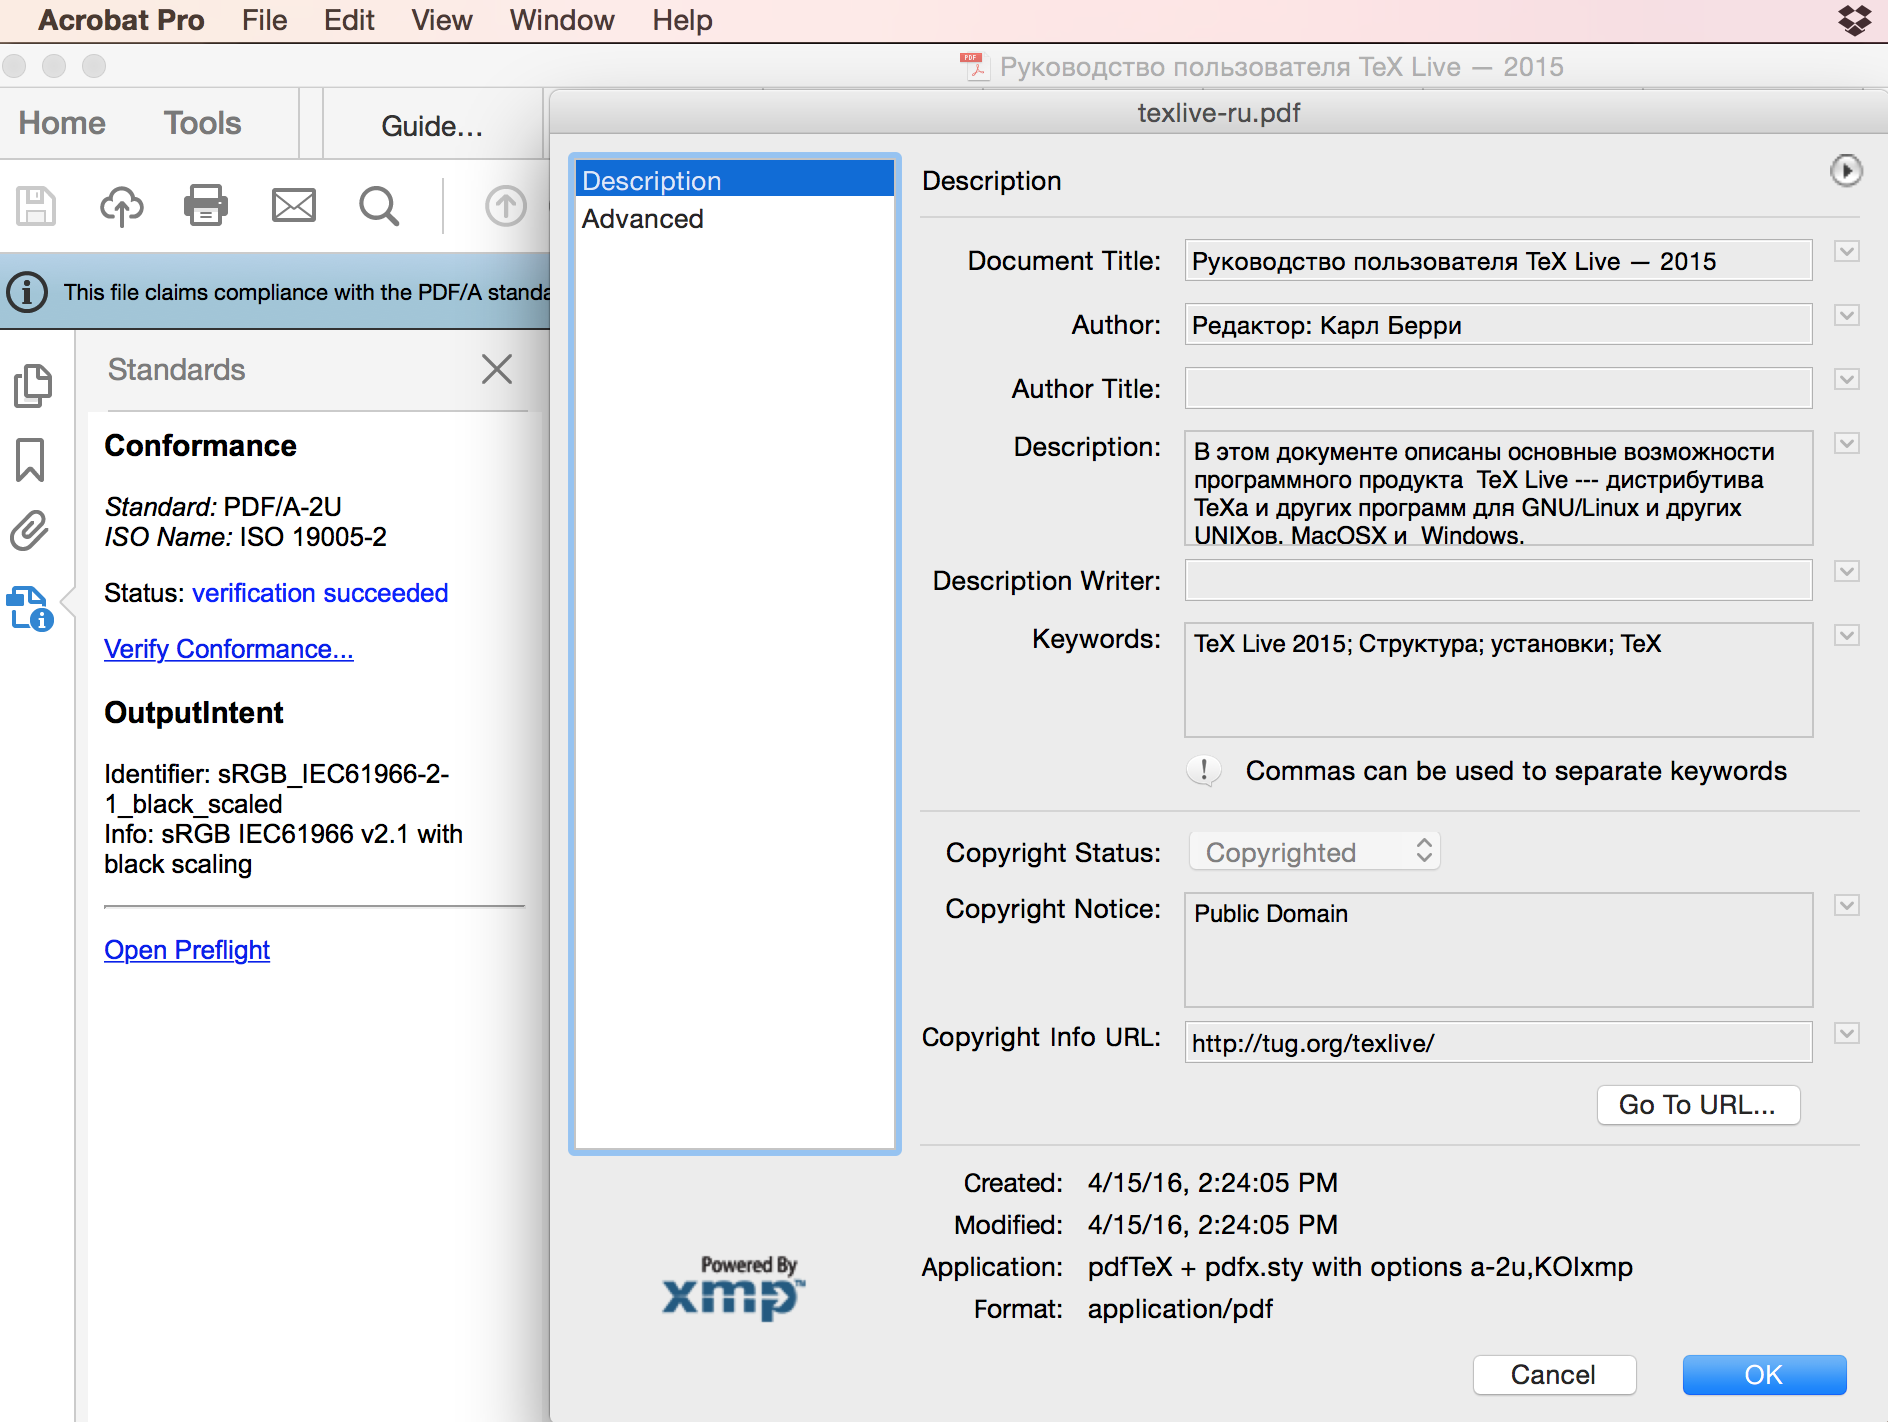
\includegraphics[scale=.33]{TL-RU-metadata}
% \caption{Metadata generated from the coding shown in Figure\,\ref{koi8-code},
%  viewed using Acrobat Pro's `Additional Metadata \dots' panel.}\label{koi8-meta}
% \end{figure}
% \begin{figure}[htb]
% {\UseRawInputEncoding
% \begin{decl}[]
%  |% $Id: texlive-ru.tex 34060 2014-05-16 19:52:41Z boris $|\\
|% |\\
|%\def\Status{1}|\\
|\providecommand{\pdfxopts}{a-2u,KOIxmp}|\\
|\providecommand{\thisyear}{2015}|\\
|%\immediate\write18{rm \jobname.xmpdata}%  uncomment for Unix-based systems |\\
|\begin{filecontents*}{\jobname.xmpdata}|\\
|\Title{\textKOI{����������� ������������} TeX Live \textemdash \thisyear}|\\
|\Author{\textKOI{��������: ���� �����}}|\\
|\Subject{\textKOI{� ���� ��������� ������� �������� ����������� ������������ �������� } |\\
| TeX Live \textKOI{--- ������������ }TeX\textKOI{� � ������ �������� ���} GNU/Linux |\\
| \textKOI{� ������ }UNIX\textKOI{��}, MacOSX\textKOI{ �  Windows.}}|\\
|\Keywords{TeX Live \thisyear\sep \textKOI{���������}\sep \textKOI{���������}\sep \TeX}|\\
|\CoverDisplayDate{\textKOI{���} \thisyear}|\\
|\CoverDate{2015-05-06}|\\
|\Copyrighted{False}|\\
|\Copyright{Public Domain}|\\
|\CopyrightURL{http://tug.org/texlive/}|\\
|\Creator{pdfTeX + pdfx.sty with options \pdfxopts }|\\
|\end{filecontents*}|\\
|\documentclass{article}|\\
|\usepackage[\pdfxopts]{pdfx}[2016/03/09]|\\
|\PassOptionsToPackage{obeyspaces}{url}|\\
|\let\tldocrussian=1  % for live4ht.cfg |\\
|\usepackage{cmap}|\\
|\usepackage{tex-live}|\\
|\usepackage[koi8-r]{inputenc}|\\
|\usepackage[russian]{babel}|\\
| ... |\\
|\begin{document}|\\
|\title{%|\\
|  {\huge \textit{����������� ������������ \protect\TL{} "--- \thisyear}}%|\\
|}|\\
|\author{��������: ���� �����\\[3mm]|\\
|        \url{http://tug.org/texlive/}}|\\
|\date{��� \thisyear}|

% \end{decl}
% }%
% \setbox0=\hbox{\kern-10cm\texttt{\`{ }\^{ }\~{ }\"{ }\r{ }\^{ }\u{ }\H{ }\'{ }\k{ }\v{ }\.{ }\i}}%
% \ht0=0pt\dp0=0pt\box0\vskip-\baselineskip
% \caption{Example of cyrillics in metadata, shown as if \texttt{T1}-encoded.
%  See Figure\,\ref{koi8-meta} for the actual result.}\label{koi8-code}
% \end{figure}
%
% \subsubsection[Metadata with Cyrillics]{Metadata with Cyrillics}\label{sssec-cyr}
%
% Here is a `real-world' example, with Figure\,\ref{koi8-meta} showing the metadata
% as could be produced for the Russian language version of the \TeX\ Live documentation,
% from coding as shown in Figure\,\ref{koi8-code}.
% The source file itself is actually encoded for KOI8-R, as indicated by the presence
% of the code line |\usepackage[koi8-r]{inputenc}|, 
% but is deliberately shown here encoded as |T1|~\cite[p.\,449]{LC2}.
% This difference is immaterial for checking the validity of the metadata.
% For example, the stream of upper (accents, etc.) characters within
% |\Title{\textKOI{ ... }}| is the same as within |\title{...\textit{ ... }}|.
% Similarly for |\Author{\textKOI{...}}| and |\author{...}|, and |\CoverDate| and |\date|.
% Strings for the |\Subject| and |\Keywords| are taken from the first actual paragraph
% in the document, and from early subsection titles.
%
% It is the `parser' command/macro |\textKOI{ ... }| that indicates that the upper range
% characters (having byte codes 128--255) are to be treated as KOI8-R characters, 
% rather than as part of UTF-8 byte sequences. It works by examining each byte in sequence,
% and returning the appropriate UTF-8 2-byte sequence for the required cyrillic character. 
% This happens during the processing of data from |\jobname.xmpdata| for fleshing-out 
% the XMP metadata packet to be included within the final PDF/A document.
%
% The `parser' macros defined for various encodings, are given in Figure\,\ref{parsers}.
% In Section\,\ref{ssec-xmplang} the package options are given 
% for loading the appropriate support for desired languages or alphabets.
% Support for other encodings can be added, if there proves to be a need.
% 
%\begin{figure}[ht]
% \centering
% \begin{tabular}{lll}\hline
%  macro & encodings & bytes 128--255 with languages\\\hline
%  |\textLAT| & Latin-1 & Western European \\
%  |\textLII| & Latin-2 & Middle European \\
%  |\textLIII| & Latin-3 & South European \\
%  |\textLIV| & Latin-4 & North European \\
%  |\textLTV| & Latin-5 & Turkish \\
%  |\textLVI| & Latin-6 & Nordic \\
%  |\textLVII| & Latin-7 & Baltic Rim \\
%  |\textLIIX| & Latin-8 & Celtic \\
%  |\textLIX| & Latin-9 & Western European, incl. \texteuro \\
%  |\textKOI| & KOI8-R, KOI8-RU & cyrillic alphabets \\
%  |\textLGR| & LGR, ISO-8859-7 & Greek \& Polytonic Greek\\
%  |\textARM| & Arm\TeX, ArmSCII8 & Armenian\\
%  |\textHEB| & HE8, ISO-8859-8, CP1255 & Hebrew\\
%  |\textHEBO| & CP862 & Hebrew\\
%  |\(...\)| & parses simple mathematical expressions\\\hline
% \end{tabular}
% \caption{Parser macros, defined for specific types of input.}\label{parsers}
% \end{figure}
% \begin{figure}[hbt]
% \centering
% 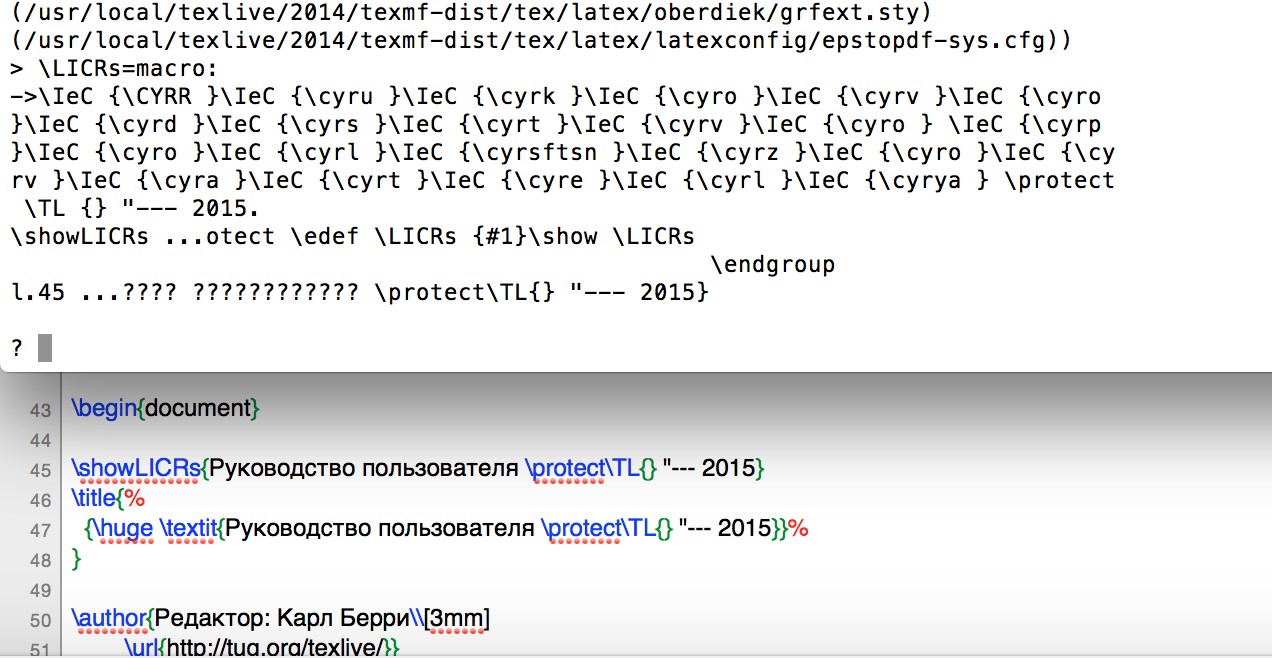
\includegraphics[scale=.5]{TL-RU-LICRs}
% \caption{How to see LICRs in the \texttt{.log} window.}\label{koi8-LICR}
% \end{figure}
%
% With encoded characters marked in this way with a `parser' macro, 
% it is actually possible to mix UTF-8 metadata with other bytes;
% provided, of course, you have an editor that allows such a file
% to be created and saved. On the other hand, if you are unhappy with mixing
% content having different encodings, then there is another way, based upon
% \LaTeX's LICR macros~\cite[\S\,7.11]{LC2} for representing accented 
% and non-latin characters. 
% These are normally hidden away (`I $=$ Internal') but in fact can be seen
% within auxiliary files, such as |.aux| and |.toc|, |.lof| and |.lot|.
% This is how \LaTeX\ stores the knowledge of such characters for use in
% a part of the document processing which may not have the same encoding
% as the document as a whole, or may require characters generated using several
% different encodings. Thus LICRs allow for a reliable representation
% passed to a different context; think `I $=$ Interchange'.
%
% \begin{figure}[hbt]
% {\UseRawInputEncoding
% \begin{decl}[]
% |% $Id: texlive-ru.tex 34060 2014-05-16 19:52:41Z boris $|\\
|% |\\
|%\def\Status{1}|\\
|\providecommand{\pdfxopts}{a-2u,KOIxmp}|\\
|\providecommand{\thisyear}{2015}|\\
|%\immediate\write18{rm \jobname.xmpdata}%  uncomment for Unix-based systems |\\
|\begin{filecontents*}{\jobname.xmpdata}|\\
|\Title{\IeC {\CYRR }\IeC {\cyru }\IeC {\cyrk }\IeC {\cyro }\IeC {\cyrv }\IeC {\cyro }|\\
| \IeC {\cyrd }\IeC {\cyrs }\IeC {\cyrt }\IeC {\cyrv }\IeC {\cyro } \IeC {\cyrp }\IeC {\cyro }|\\
| \IeC {\cyrl }\IeC {\cyrsftsn }\IeC {\cyrz }\IeC {\cyro }\IeC {\cyrv }\IeC {\cyra }\IeC {\cyrt }|\\
| \IeC {\cyre }\IeC {\cyrl }\IeC {\cyrya } TeX Live \textemdash \thisyear}|\\
|\Author{\IeC {\CYRR }\IeC {\cyre }\IeC {\cyrd }\IeC {\cyra }\IeC {\cyrk }\IeC {\cyrt }|\\
| \IeC {\cyro }\IeC {\cyrr }: \IeC {\CYRK }\IeC {\cyra }\IeC {\cyrr }\IeC {\cyrl } |\\
| \IeC {\CYRB }\IeC {\cyre }\IeC {\cyrr }\IeC {\cyrr }\IeC {\cyri }|\\
|\Keywords{TeX Live \thisyear\sep \IeC {\CYRS }\IeC {\cyrt }\IeC {\cyrr }\IeC {\cyru }|\\
| \IeC {\cyrk }\IeC {\cyrt }\IeC {\cyru }\IeC {\cyrr }\IeC {\cyra }\sep \IeC {\cyru }|\\
| \IeC {\cyrs }\IeC {\cyrt }\IeC {\cyra }\IeC {\cyrn }\IeC {\cyro }\IeC {\cyrv }\IeC {\cyrk }|\\
| \IeC {\cyri }\sep \TeX}|\\
|\Subject{\IeC {\CYRV } \IeC {\cyrerev }\IeC {\cyrt }\IeC {\cyro }\IeC {\cyrm } \IeC {\cyrd }|\\
| \IeC {\cyro }\IeC {\cyrk }\IeC {\cyru } ... |\\
| ... |\\
|\CoverDisplayDate{\IeC {\CYRM }\IeC {\cyra }\IeC {\cyrishrt } 2015}|\\
|\CoverDate{2015-05-06}|\\
|\Copyrighted{False}|
\endinput
|\Copyright{Public Domain}|\\
|\CopyrightURL{http://tug.org/texlive/}|\\
|\Creator{pdfTeX + pdfx.sty with options \pdfxopts }|\\
|\end{filecontents*}|\\
|\documentclass{article}|\\
|\usepackage[\pdfxopts]{pdfx}[2016/03/09]|\\
|\PassOptionsToPackage{obeyspaces}{url}|\\
|\let\tldocrussian=1  % for live4ht.cfg |\\
|\usepackage{cmap}|\\
|\usepackage{tex-live}|\\
|\usepackage[koi8-r]{inputenc}|\\
|\usepackage[russian]{babel}|\\
| ... |\\
|\begin{document}|\\
|\title{%|\\
|  {\huge \textit{����������� ������������ \protect\TL{} "--- \thisyear}}%|\\
|}|\\
|\author{��������: ���� �����\\[3mm]|\\
|        \url{http://tug.org/texlive/}}|\\
|\date{��� \thisyear}|

% \end{decl}
% }%
% \caption{Example of cyrillics in metadata, using LICRs.}\label{koi8-code2}
% \end{figure}
% \begin{figure}[htbp]
% \centering
% 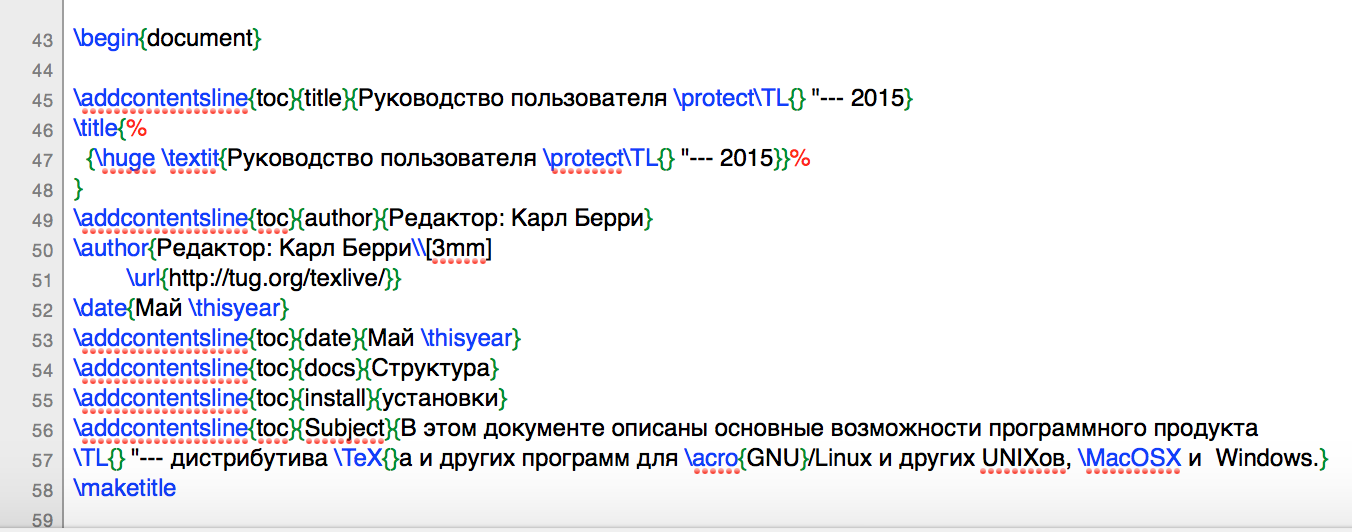
\includegraphics[scale=.5]{TL-RU-toc}
% \caption{How to get desired LICRs into the \texttt{.toc} file.}\label{koi8-toc}
% \end{figure}
%
% Figure~\ref{koi8-LICR} shows how to see this. 
% The document source in the lower portion clearly shows the cyrillic
% input, whereas the |.log| messages in a command-line window above
% reveal the LICR representation. A command |\showLICRs| is available
% with |pdfx.sty| version 1.5.8, specifically to allow this.
% Now the LICR representation can be copied directly from the |.log| file, 
% modulo slight difficulties due to the way long lines are broken.
% As this representation is entirely with ASCII characters, it should not
% cause any conflict with any UTF-8 metadata that you want within the same file.
% The |.xmpdata| file might now look as in Figure~\ref{koi8-code2}.
% Although very verbose, this should be resistant to any corruption due to
% character encodings, and produces the same result within the PDF, 
% as in Figure~\ref{koi8-meta}.
% 
% Alternatively one can exploit the |.toc| file, using \LaTeX's command
% |\addtocontents|, as shown in Figure~\ref{koi8-toc}.
% After processing the file, you can copy the LICR representations out
% of the |.toc| file, taking care to remove anything of a non-character
% nature (e.g., implementing the size and spacing of the letters in \TeX).
%
% Of course once you have harvested the metadata in this format, remove
% or comment-out those extra |\showLICRs| to get uninterrupted processing.
% Similarly comment-out the extra |\addtocontents| lines, else the real 
% Table-of-Contents will become corrupted with unwanted entries.
% A couple more \LaTeX\ processing runs should restore the PDF to the
% way you want it.
%
% \subsubsection[Metadata with Polish]{Metadata with Polish}\label{sssec-pol}
% 
% The next example has upper-range bytes intended to represent Latin-2 encoded 
% characters, as used in Polish. 
% With the \LaTeX\ source starting as in Figure~\ref{tldoc-pol}, 
% the resulting metadata is shown in Figure~\ref{tlmeta-pol}.
% 
%\begin{figure}[htb]
% \centering
% 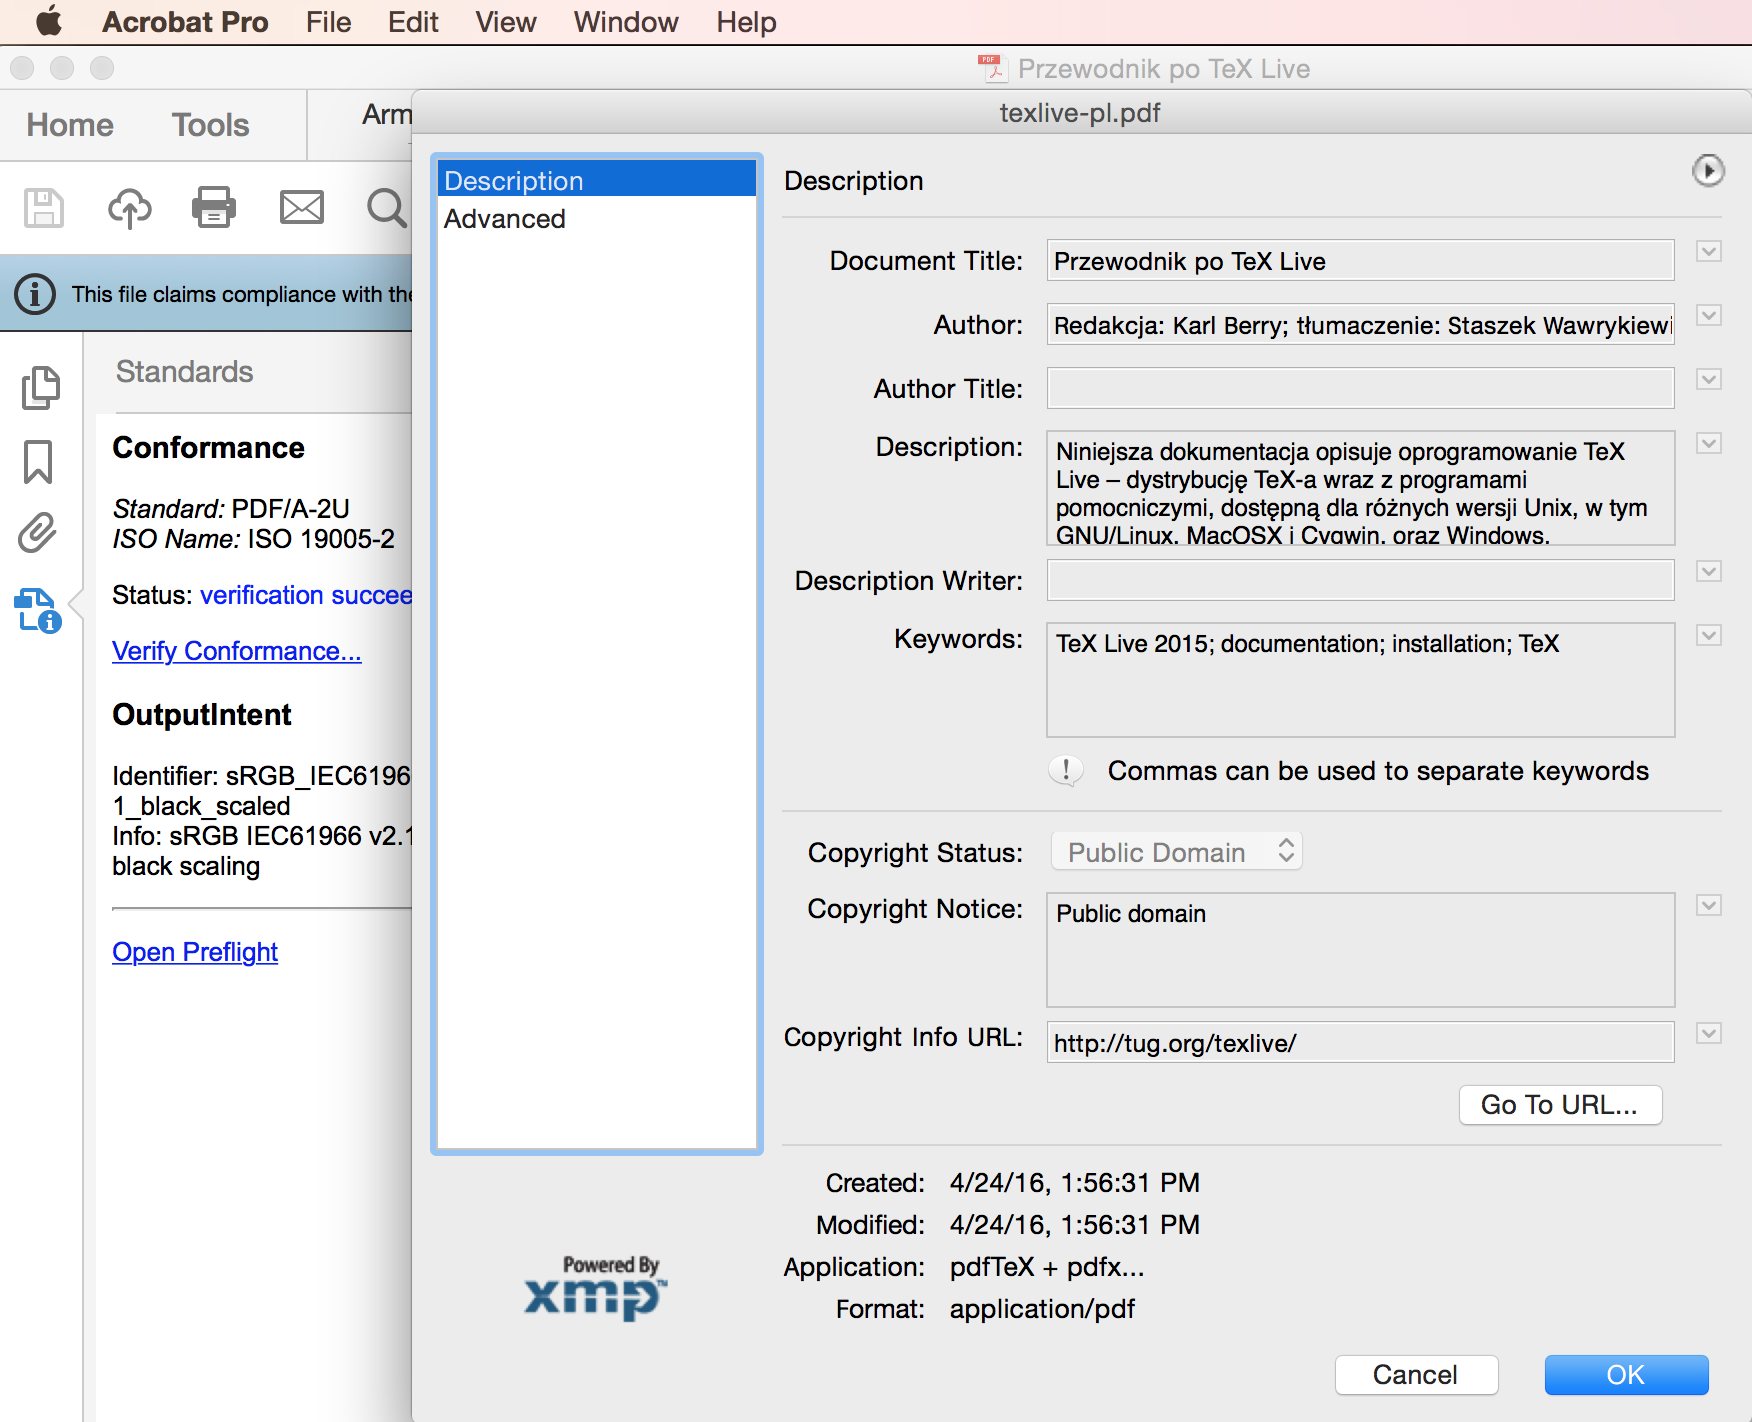
\includegraphics[scale=.45]{TL-POL-meta}
%\caption{Metadata generated from the coding shown in Figure~\ref{tldoc-pol}
% for the Polish version of \TeX\ Live 2015 documentation, showing Latin-2 encoded 
% characters. The document is valid for PDF/A-2, after having been processed with 
% pdf-\LaTeX.}\label{tlmeta-pol}
%\end{figure}
%
%\begin{figure}[!htp]
% {\UseRawInputEncoding
%\begin{decl}[]
% |% iso8859-2|\\
|% $Id: texlive-pl.tex, v. 53 2015/05/17|\\
|% TeX Live documentation.|\\
|% Originally written by Sebastian Rahtz and Michel Goossens,|\\
|% now maintained by Karl Berry and others.|\\
|% Polish translation and additions by Staszek Wawrykiewicz|\\
|% (with a little help from my friends, while my guitar gently weeps ;-)|\\
|% Public domain.|\\
|%  ----|\\
|% UWAGA dla recenzent�w/t�umaczy:  %%! to moje komentarze (StaW)|\\
|% |\\
|\providecommand{\pdfxopts}{a-2u,LATxmp}|\\
|\providecommand{\thisyear}{2015}|\\
|\begin{filecontents*}{\jobname.xmpdata}|\\
|\Title{Przewodnik po TeX Live \thisyear}|\\
|\Author{Redakcja: Karl Berry\sep \textLII{t�umaczenie: Staszek Wawrykiewicz}}|\\
|\Subject{\textLII{Niniejsza dokumentacja opisuje oprogramowanie \TeX\ Live |\\
| -- dystrybucj� \TeX-a wraz z~programami pomocniczymi, dost�pn� dla r�nych wersji Unix,|\\
|  w~tym GNU/Linux, MacOSX i~Cygwin, oraz Windows.}\textLF\textLF Documentation originally|\\
| written by Sebastian Rahtz and Michel Goossens, now maintained by Karl Berry and others.}|\\
|\Keywords{TeX Live \thisyear\sep documentation\sep installation\sep \TeX}|\\
|\Copyright{Public domain}\Copyrighted{False}|\\
|\CopyrightURL{http://tug.org/texlive/}|\\
|\CoverDisplayDate{Maj \thisyear}|\\
|\CoverDate{\thisyear-05-17}|\\
|\Creator{pdfTeX + pdfx.sty with options \pdfxopts, from TeX Live 2016}|\\
|\end{filecontents*}|\\
|% |\\
|\documentclass{article}|\\
|\let\tldocenglish=0 % for live4ht.cfg|\\
|\let\textsl\textit|\\
|\usepackage[\pdfxopts]{pdfx}[2016/04/13]|\\
|\PassOptionsToPackage{obeyspaces}{url}|\\
|\PassOptionsToPackage{breaklinks,colorlinks,linkcolor=hypercolor,citecolor=hypercolor,%|\\
|  urlcolor=hypercolor,filecolor=hypercolor,bookmarksopen,hyperindex}{hyperref}|\\
|\hypersetup{breaklinks,colorlinks,allcolors=hypercolor}|\\
|\usepackage{tex-live}|\\
|\usepackage{polski}            %% for PL|\\
|\usepackage[latin2]{inputenc}  %% for PL|\\
|\usepackage[T1]{fontenc}|\\
|...|\\
|\begin{document}|\\
|\title{\huge \textit{Przewodnik po \protect\TL{} 2015}}|\\
|\author{Redakcja: Karl Berry; t�umaczenie: Staszek Wawrykiewicz \\[3mm]|\\
|        \url{http://tug.org/texlive/}}|\\
|\date{Maj 2015}|

%\end{decl}
% }%
%\caption{Start of the \LaTeX\ source for the Polish version of \TeX\ Live 
% documentation. Although Latin-2 encoded, the bytes are shown here using 
% \LaTeX's \texttt{T1} encoding \cite[p.\,449]{LC2}.}\label{tldoc-pol}
%\end{figure}
%
% Here the `parser macro' is |\textLII|, which can be seen in Figure~\ref{tldoc-pol}
% to surround either complete metadata entries, or just those parts containing 
% polish accented (or other) characters in entries that also contain english words.
% The macro |\textLF| provides a line-feed character for the UTF-8 output.
%
% As a technical note, the |\jobname.xmpdata| file is read with |\obeyspaces|
% in effect. This causes space runs in the input to be replaced by a single
% `active space' character, which ultimately expands into a normal space upon output.
% This is needed to preserve inter-word spaces, which would otherwise
% get lost during parsing, due to \TeX's pattern matching when reading macro arguments.
% Each byte is examined individually, with normal letters |a-zA-Z| and most punctuation
% characters passed through unchanged.
%
% \medskip\goodbreak
% Let's understand better how this example was created. There are three files involved.
%\begin{itemize}
% \item |pdfx.dtx|, the source for this documentation, open in an editor with
% encoding declared as UTF-8; 
% \item |texlive-pl.tex| the Polish documentation for \TeX\ Live, open in the
% same editor with Latin-2 encoding;
% \item |latin2-example.tex| which starts life as an empty file on disk.
%\end{itemize}
% \noindent
% This latter file must be opened in the editor, with encoding declared as 
% Latin-2 (ISO-8859-2).
% Next the preamble is copied from |texlive-pl.tex| and pasted into |latin2-example.tex|
% which is then saved to disk. Further editing is done to |latin2-example.tex| to
% add verbatim markers (\texttt{$\vert$...$\vert$}) and adjust line lengths for display
% within Figure~\ref{tldoc-pol}. This file's contents is included as part of the 
% documentation via ||% iso8859-2|\\
|% $Id: texlive-pl.tex, v. 53 2015/05/17|\\
|% TeX Live documentation.|\\
|% Originally written by Sebastian Rahtz and Michel Goossens,|\\
|% now maintained by Karl Berry and others.|\\
|% Polish translation and additions by Staszek Wawrykiewicz|\\
|% (with a little help from my friends, while my guitar gently weeps ;-)|\\
|% Public domain.|\\
|%  ----|\\
|% UWAGA dla recenzent�w/t�umaczy:  %%! to moje komentarze (StaW)|\\
|% |\\
|\providecommand{\pdfxopts}{a-2u,LATxmp}|\\
|\providecommand{\thisyear}{2015}|\\
|\begin{filecontents*}{\jobname.xmpdata}|\\
|\Title{Przewodnik po TeX Live \thisyear}|\\
|\Author{Redakcja: Karl Berry\sep \textLII{t�umaczenie: Staszek Wawrykiewicz}}|\\
|\Subject{\textLII{Niniejsza dokumentacja opisuje oprogramowanie \TeX\ Live |\\
| -- dystrybucj� \TeX-a wraz z~programami pomocniczymi, dost�pn� dla r�nych wersji Unix,|\\
|  w~tym GNU/Linux, MacOSX i~Cygwin, oraz Windows.}\textLF\textLF Documentation originally|\\
| written by Sebastian Rahtz and Michel Goossens, now maintained by Karl Berry and others.}|\\
|\Keywords{TeX Live \thisyear\sep documentation\sep installation\sep \TeX}|\\
|\Copyright{Public domain}\Copyrighted{False}|\\
|\CopyrightURL{http://tug.org/texlive/}|\\
|\CoverDisplayDate{Maj \thisyear}|\\
|\CoverDate{\thisyear-05-17}|\\
|\Creator{pdfTeX + pdfx.sty with options \pdfxopts, from TeX Live 2016}|\\
|\end{filecontents*}|\\
|% |\\
|\documentclass{article}|\\
|\let\tldocenglish=0 % for live4ht.cfg|\\
|\let\textsl\textit|\\
|\usepackage[\pdfxopts]{pdfx}[2016/04/13]|\\
|\PassOptionsToPackage{obeyspaces}{url}|\\
|\PassOptionsToPackage{breaklinks,colorlinks,linkcolor=hypercolor,citecolor=hypercolor,%|\\
|  urlcolor=hypercolor,filecolor=hypercolor,bookmarksopen,hyperindex}{hyperref}|\\
|\hypersetup{breaklinks,colorlinks,allcolors=hypercolor}|\\
|\usepackage{tex-live}|\\
|\usepackage{polski}            %% for PL|\\
|\usepackage[latin2]{inputenc}  %% for PL|\\
|\usepackage[T1]{fontenc}|\\
|...|\\
|\begin{document}|\\
|\title{\huge \textit{Przewodnik po \protect\TL{} 2015}}|\\
|\author{Redakcja: Karl Berry; t�umaczenie: Staszek Wawrykiewicz \\[3mm]|\\
|        \url{http://tug.org/texlive/}}|\\
|\date{Maj 2015}|
| within an environment that handles 
% presentation aspects, and (since 2018) declares |\UseRawInputEncoding|.
%
% What \emph{cannot} be done is to paste the preamble content directly into |pdfx.dtx|.
% Consider what would then happen, using `t{\l}umaczy' (`translators', on line 10 
% following `UWAGA'). This word shows correctly in the Latin-2 encoded files. 
% It was typeset here using |\l| for the `\l' letter, having Unicode code-point 
% |Ux0142| (so UTF-8 byte pair |"C5|\,|"82|). 
% However, it occurs at slot |"B3| within Latin-2 encoding. 
% In the |T1| font encoding \cite[p.\,449]{LC2} the character glyph name 
% for slot |"B3| is |/scedilla|, which is what shows in Figure~\ref{tldoc-pol}. 
% When the `\l' is pasted directly into a UTF-8 file and shown verbatim, 
% the result is the pair of glyphs |"C5| (|/Aring|) and |"82| (|/Cacute|); 
% \emph{viz.} {\UseRawInputEncoding |tłumaczy|}.
%
% As with Figure~\ref{koi8-code} it is not important that the correct characters
% are shown here, but that the metadata in |\jobname.xmpdata| corresponds to what
% is used on the titlepage of the PDF; e.g., the contents of |\Title| and |\title|,
% |\Author| and |\author|, etc.
% 
%
% \subsubsection[Metadata with Greek]{Metadata with Greek}\label{sssec-grk}
%
%\begin{figure}[!hb]
% \centering
% 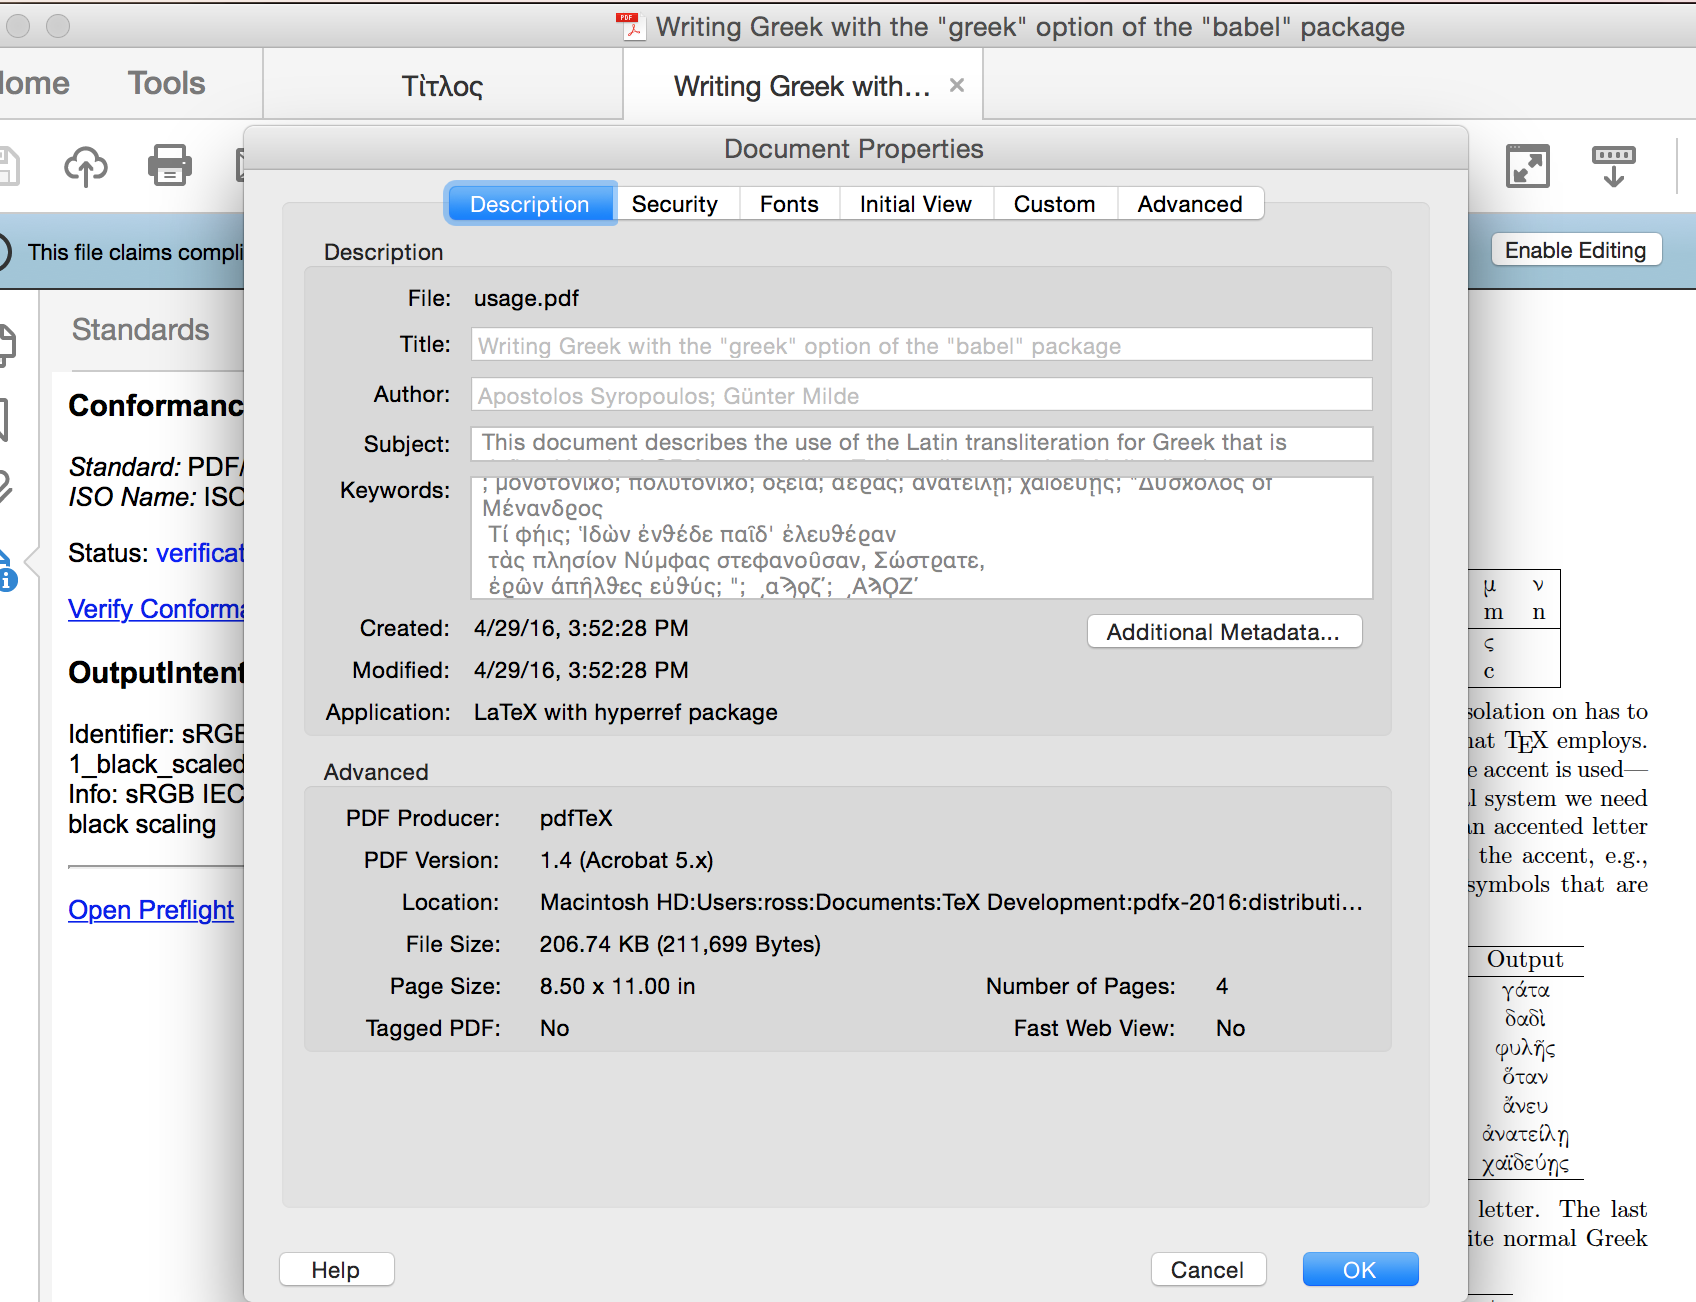
\includegraphics[scale=.43]{usage-meta}
%\caption{Metadata generated from the coding shown in Figure~\ref{greek-code}
% using the greek language specified via the LGR encoding.}\label{greek-meta}
%\end{figure}
%
%\begin{figure}[!htp]
%\begin{decl}[]
%|% ... |\\
%|% This file is part of the Babel system.|\\
%|% --------------------------------------|\\
%|% |\\
%|% It may be distributed and/or modified under the |\\
%|% conditions of the LaTeX Project Public License, either version 1.3|\\
%|% ... |\\
%{\color{verbcolor}\texttt{\% The Current Maintainer of this work is G\"unter Milde.}}\\
%|% ... |\\
%| |\\
%|\providecommand{\pdfxopts}{a-2u,LGRxmp,LATxmp}|\\
%|\begin{filecontents*}{\jobname.xmpdata}|\\
%|\Title{Writing Greek with the "greek" option of the "babel" package}|\\
%{\color{verbcolor}\texttt{\string\Author\{Apostolos Syropoulos\string\sep\ G\"unter Milde\}}}\\
%|\Subject{This document describes the use of the Latin transliteration for Greek that is |\\
%| defined by the LGR font encoding. Today, all modern LaTeX distributions support literal|\\
%| input of Greek, which is the preferred method for new documents. [G. Milde 2013/12/02]}|\\
%|\Keywords{\textLGR{monotonik'o}\sep \textLGR{polutonik'o}\sep \textgreek{oxe'ia} \sep |\\
%{\catcode `\|=11 \color{verbcolor}
%\texttt{\ \ \string\textgreek\{>a'erac\}\string\sep\ \string\textgreek\{>anate'ilh|\}\string\sep\ \string\textgreek\{qa"ide'uh|c\}\}}}| \sep |\\
%|  \textgreek{D'uskoloc} of \textgreek{M'enandroc}\textLF \textLGR{T'i f'hic? <Id`wn |\\
%|  >enj'ede pa~id'' >eleuj'eran\textLF t`ac plhs'ion N'umfac stefano~usan, S'wstrate,|\\
%|  \textLF >er~wn 'ap~hljec e>uj'uc? \sep |\\
%|  \textaristerikeraia\textalpha\textsampi\textqoppa\textzeta\textdexiakeraia\sep |\\
%|  \textaristerikeraia\textAlpha\textSampi\textQoppa\textZeta\textdexiakeraia}}|\\
%|\CoverDate{1997-10-15}|\\
%|\CoverDisplayDate{October 15, 1997}|\\
%|\Copyright{This file is part of the Babel system.\textLF This file may be distributed and/or|\\ 
%| modified under the conditions of the LaTeX Project Public License, either version 1.3 |\\
%| of this license or (at your option) any later version.}|\\
%|\CopyrightURL{http://www.latex-project.org/lppl.txt}|\\
%|\end{filecontents*}|\\
%|%|\\
%|\documentclass[11pt]{article}|\\
%|\usepackage[\pdfxopts]{pdfx}[2016/04/13]|\\
%|\hypersetup{colorlinks,allcolors=blue}|\\
%|\usepackage[american,greek]{babel}|\\
%|\languageattribute{greek}{polutoniko}|\\
%|\usepackage{athnum,grmath}|\\
%|\newcommand{\sg}{\selectlanguage{greek}}|\\
%|\newcommand{\sa}{\selectlanguage{american}}|\\
%|\begin{document}|\\
%|\selectlanguage{american}|\\
%|\title{Writing Greek with the \ttfamily greek\rmfamily\  option of the |\\
%| \ttfamily babel\rmfamily\ package}|\\
%|\author{Apostolos Syropoulos\\|\\
%|        ...\\...}|\\
%|\date{October 15, 1997}|\\
%|\maketitle|\\
%|\abstract{\noindent|\\
%|This document describes the use of the Latin transliteration for Greek that|\\
%|is defined by the LGR font encoding. Today, all modern LaTeX distributions|\\
%|support literal input of Greek, which is the preferred method for new|\\
%|documents. [G. Milde 2013/12/02]}|
%\end{decl}
%\caption{Start of enriched \LaTeX\ source for a document describing how to typeset
% in Greek, with added metadata demonstrating the LGR transliteration encoding.
% }\label{greek-code}
%\end{figure}
%
% Prior to proper support for UTF-8 input, a method for preparing document source
% for the modern Greek language (and also for polytonic Greek), involved the use
% of LGR encoded fonts. Such a font has Greek (instead of Latin) letters in the 
% slots for |a-zA-Z|, see~\cite[\S9.4.2]{LC2}. Thus ordinary ASCII letters are used
% to produce the Greek characters; the mapping of ASCII to Greek is referred to as
% a `transliteration' scheme. It serves as \emph{both} an input encoding, and as 
% a font encoding. Accents and diacritic marks are provided through ligatures 
% built-in to the fonts. Various documents can be found on the web\footnote{e.g., 
% \url{http://milde.users.sourceforge.net/LGR/}} and
% within \TeX\ Live distributions\footnote{%
% TeXLive: \textcolor{urlcolor}{\texttt{.../2016/texmf-dist/doc/generic/babel-greek/}}}. 
%
% Indeed the current maintainer G\"unther Milde states
% ``The LGR transliteration does not work for PDF metadata''.
% This is because there is no translation of LGR input into \LaTeX\ LICRs,
% as happens with say |\usepackage[utf8]{inputenc}| for UTF-8 input,
% or when upper 8-bit characters are present using |\usepackage[iso-8859-7]{inputenc}|.  
% With these, LICRs such as |\textAlpha|, |\textOmicron|, \dots, |\textomega| 
% are produced, which result in the correct characters for metadata and bookmarks,
% perhaps employing Unicode `combining' characters for accented letters.
% Using |pdfx| the UTF-8 characters can be put directly into the |.xmpdata| file;
% LICRs are interpreted provided the |grkxmp| loading option has been specified.
% 
% Using the methods of |pdfx| the metadata difficulty is remedied, as can be seen in 
% Figure~\ref{greek-meta} using coding as shown in Figure~\ref{greek-code}. This requires 
% the |LGRxmp| option and |\textLGR| `parser' macro. The original document source, 
% called |usage.tex|, can be found in the directory specified in the footnote below.
% As this document is essentially an English description of how to use LGR for Greek,
% we have used the `Keywords' field to provide examples of such usage. 
% Since a macro |\textgreek| can be used for greek portions within such documents, 
% this macro name is aliased to |\textLGR| within the context where metadata is processed.
% Furthermore, parsing using |\textLGR| generates correct pre-composed characters 
% for letters with accents or diacritics. Bookmarks can also be generated from
% LGR input, using a technique described in Section~\ref{sssec-arm}.
%
% \bigskip\noindent
% The features available with different loading options are summarised here.
% \begin{itemize}
% \item 
%  no option: all metadata in |.xmpdata| file is in UTF-8 (incl. ASCII)
% \item
%  |grkxmp|: LICRs can be present; e.g. |\textAlpha|, |\textOmega|, etc. 
% \item
%  |LGRxmp|: supports LGR-encoded input and |ISO-8859-7| upper range characters,
%    using the |\textLGR| `parser' macro.         
% \end{itemize}
% With |LGRxmp| specified, the features of |grkxmp| are also available; so any 
% lower-listed option allows data to be mixed with that for higher-listed ones.
%
%
% The final piece to get validation for PDF/A from LGR input, is to specify
% a Unicode point for the `|v|' used only in the strong `|sv|' ligature to obtain 
% a non-final `sigma' typeset in isolation. 
%\begin{decl}[]
% |\pdfglyphtounicode{internalchar2}{200D}|
%\end{decl}
% This gives an interpretation as `zero-width joiner'.
% There are two instances of this within |usage.tex|. Copy/Paste works as desired.
% Using \pdftex\ the above command is done automatically. 
% Drivers, such as Xe\LaTeX\ lacking an implementation of |\pdfglyphtounicode|, 
% can fail to produce a valid PDF due to this rather minor deficiency.
% 
% Greek numerals, using |\greeknumeral| or |\Greeknumeral| cannot work directly within
% a |.xmpdata| file. However if such is desired, the following technique allows
% correct LICRs to be found for use in the metadata. 
% At any convenient place within the \LaTeX\ source; e.g., near where the required  
% number is used, insert coding such as:
% \begin{decl}[]
% |{\pdfxGreeknumeralsHack \textgreek{\edef\num{\greeknumeral{1997}}\show\num}}%|
% \end{decl}
% Upon processing, the following will be written to the console or |.log|-window.
% \begin{decl}[]
%|> \num=macro:|\\
%|->\LGR\textaristerikeraia \LGR\textalpha \LGR\textsampi \let \protect \LGR\text|\\
%|dexiakeraia \LGR\textqoppa \let \protect \LGR\textdexiakeraia \LGR\textzeta \le|\\
%|t \protect \LGR\textdexiakeraia \protect \LGR\textdexiakeraia .|\\
%|<argument> ...um {\greeknumeral {1997}}\show \num |\\
%|                                                  |\\
%|l.90 ...k{\edef\num{\greeknumeral{1997}}\show\num}|\\
%|                                                  }|\\
%|? |
% \end{decl}
% from which the desired string of LICRs, is extracted; \emph{viz}.
% \begin{decl}[]
% |\textaristerikeraia\textalpha\textsampi\textqoppa\textzeta\textdexiakeraia|
% \end{decl}
% The corresponding trick does not work with |\Greeknumeral|, but the uppercasing
% can be done manually from the string obtained using |\greeknumeral|,
% \begin{decl}[]
% |\textaristerikeraia\textAlpha\textSampi\textQoppa\textZeta\textdexiakeraia|
% \end{decl}
% leaving the initial and final |\text...keraia| macros as all lowercase.
% For smooth processing, remove or comment-out the added line after collecting the LICRs.
%
%
% \def\ArmTeX{Arm\kern -0.15em\TeX}%
% \subsubsection[Metadata with Armenian]{Metadata with Armenian}\label{sssec-arm}
% 
% \begin{figure}[!htbp]
% \centering
% 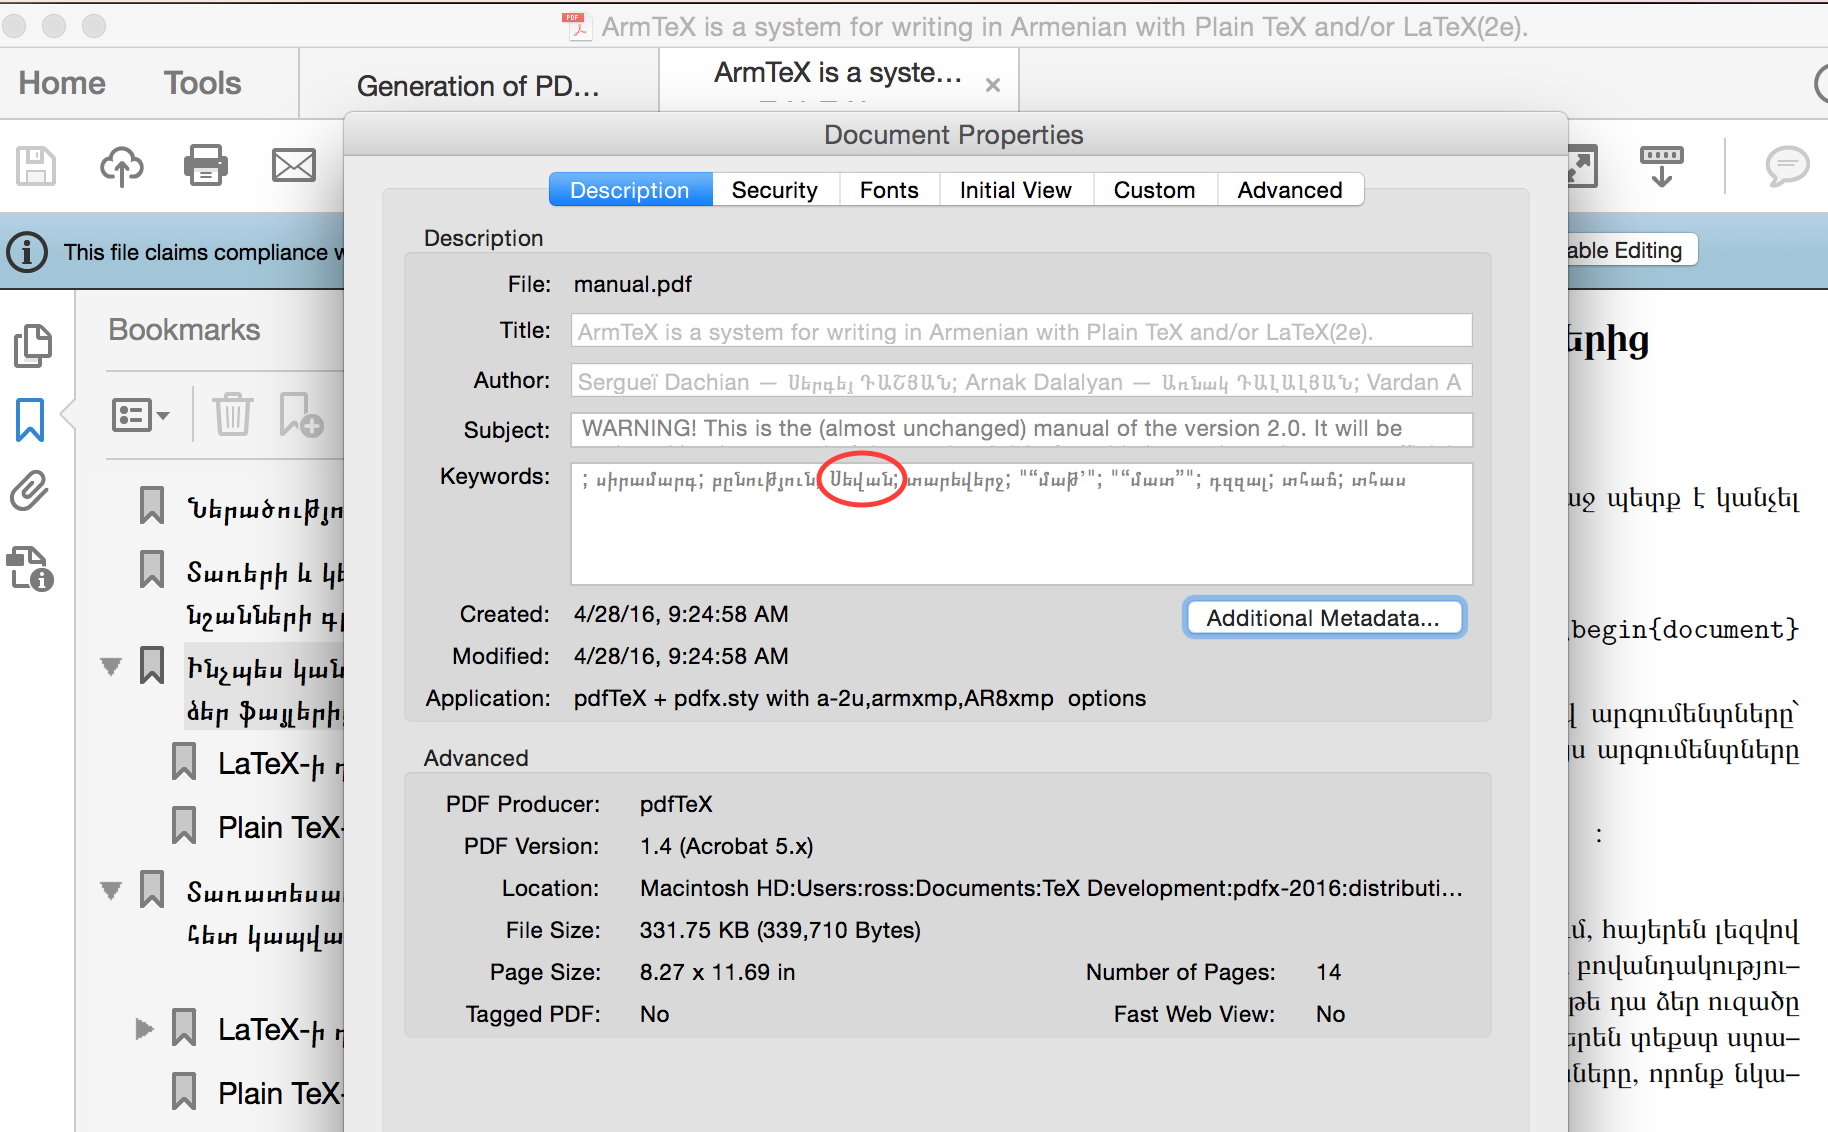
\includegraphics[scale=.42]{armtex-meta}
%\caption{Metadata generated from the coding shown in Figure~\ref{arm-code}
% using the Armenian language specified using \ArmTeX\ transliteration.
% Bookmarks have been generated in Armenian. Figure ~\ref{ex-arm} explains
% how the word indicated in red is obtained via parsing.}\label{arm-meta}
% \end{figure}
%
% \begin{figure}[!htbp]
%  \let\small\scriptsize
% {\UseRawInputEncoding
% \begin{decl}[]
% |%%%%%%%%%%%%%%%%%%%%%%%%%%%%%%%%%%%%%%%%%%%%%%%%%%%%%%%%%%%%%%%%%%%%%%%%%%%%%%|\\
|%%|\\
|%% This is the `manual.tex' file (ArmTeX manual in Armenian).|\\
| ... |\\
|%%|\\
|%%%%%%%%%%%%%%%%%%%%%%%%%%%%%%%%%%%%%%%%%%%%%%%%%%%%%%%%%%%%%%%%%%%%%%%%%%%%%%|\\
|\providecommand{\pdfxopts}{a-2u,armxmp,AR8xmp}|\\
|\immediate\write18{rm \jobname.xmpdata}|\\
|\begin{filecontents*}{\jobname.xmpdata}|\\
|\Title{ArmTeX is a system for writing in Armenian with Plain TeX and/or LaTeX(2e).\textLF|\\
| \textARM{\ArmTeX` {\aroff\TeX}-um ev {\aroff\LaTeX}-um Hayeren Lezvov Grelu Hamakarg}}|\\
|\Author{Sergue\"i Dachian \textARM{--- Sergey DASHYAN}\sep Arnak Dalalyan |\\
| \textARM{--- Ar'nak DALALYAN}\sep Vardan Akopian \textARM{--- Vardan HAKOBYAN}}|\\
|\Copyright{\textcopyright 1997\textendash 2013  ArmTeX may be distributed and/or modified  |\\
| under the conditions of the LaTeX Project Public License, either version 1.3 of this  |\\
| license or (at your option) any later version.}|\\
|\CopyrightURL{http://www.latex-project.org/lppl.txt}|\\
|\Subject{WARNING! This is the (almost unchanged) manual of the version 2.0. It will be |\\
| replaced by the manual of the version 3.0 before this beta release becomes official. |\\
| A (temporary) brief description of the new features of \latArmTeX~3.0 can be found at |\\
| the end of the ``readme.txt'' file. \textLF|\\
{\catcode`\|=12 \color{verbcolor}\texttt{ \string\textLF\string\textARM%
 \{OWSHADROWT'YO|WN:}} |Sa tarberak 2.0-i (grethe anphophox) dzer'narkn e': Ayn |\\
| kphoxarinvi tarberak 3.0-i dzer'narkov naxqan ays beta tho\-ghark\-man pashtonakanacowmu': |\\
| \ArmTeX~3.0-i nor hnaravoruthyunneri (g'a\-ma\-na\-ka\-vor) hamar'ot nkaragrowmu' (angleren|\\
| lezvov) karogh eq gu't\armuh nel~``}readme.txt\textARM{'' fayli verjum:}|\\
| \textLF\textLF\textARM{Hamakargu' o'gtagorc'elu hamar bavakan e' karoghanal ayn kanchel dzer|\\
| fayleric, tirapetel tar'qatesakneru' phoxogh hramannerin ev i\-ma\-nal the inchpes petq e' |\\
| nermuc'el teqstu' steghnasharic: Ays gor\-c'o\-ghu\-thyun\-ne\-ru' nkaragrvac' en hajordogh |\\
| ereq bag'innerum:}}|\\
|\Keywords{\textARM{si\-ra\-marg}\sep \textARM{bu'\armuh nuthyun}\sep \textARM{Se\armuh van}|\\
| \sep \textARM{tare\*verj}\sep \textARM{``mat''}\sep \textARM{``mat"}\sep \textARM{d\*zzal}|\\
| \sep \textARM{t\*haj'}\sep \textARM{t\*has}}|\\
|\CoverDisplayDate{1 June 1999 (\textARM{1-u' hunisi 1999 th.})}|\\
|\Creator{pdfTeX + pdfx.sty with \pdfxopts\space options}|\\
|\pdfxEnableCommands{\let\sl\empty%|\\
| \xdef\sectAtitle{\textARM{Nerac'uthyun}}%|\\
| \xdef\sectBtitle{\textARM{Tar'eri ev ketadrakan nshanneri greladzevu'}}%|\\
| ... |\\
| \xdef\sectFtitle{\textARM{Arm\TeX-i phophoxman patmuthyunu'}}%|\\
|}|\\
|\end{filecontents*}|\\
| |\\
|\documentclass[12pt,a4paper]{article}|\\
|\usepackage[\pdfxopts]{pdfx}|\\
|\hypersetup{colorlinks,allcolors=blue}|\\
| ... |\\
|\title{\ArmTeX$\,$` $\,${\aroff \TeX}-um ev {\aroff \LaTeX}-um Hayeren Lezvov |\\
|  Grelu Hamakarg\\ {\normalsize\aroff (\latArmTeX: a System for Writing in Armenian |\\
|  with \TeX\ and \LaTeX)}}|\\
|\author{ ... }%|\\
|\date{1-u' hunisi 1999 th.}|\\
| ... |\\
|\begin{document}|\\
|\maketitle|\\
| ... |\\
|%\section{\sectAtitle}%{Nerac'uthyun}}|\\
|\pdfxBookmark{\section}{\sectAtitle}{Nerac'uthyun}|\\
| |
%
% \end{decl}
% }%
% \caption{Enriched \LaTeX\ source for the Armenian version of the \ArmTeX\ manual,
% with added metadata demonstrating the \ArmTeX\ transliteration scheme for \texttt{OT6} encoding.
% Also shown is coding used to produce bookmarks from the transliteration.}\label{arm-code}
% \end{figure} 
% 
% The \ArmTeX\ package\footnote{documentation: %
%  TeXLive: \textcolor{urlcolor}{\texttt{.../2016/texmf-dist/doc/generic/armenian/}}}
% provides the method to typeset Armenian, with input being specified in various ways 
% including a transliteration scheme from ASCII input. This transliteration is directed 
% at the use of the |OT6| encoding, developed for this purpose.
% Each way is supported by |pdfx.sty| with appropriate loading options, similar
% to the support for Greek~(see Section~\ref{sssec-grk}). 
% \begin{itemize}
% \item 
%  no option: all metadata in |.xmpdata| file is in UTF-8 (incl. ASCII)  
% \item
%   |armxmp|: using LICR-like macro names; e.g. |\armAyb|, |\armsha|, |\armfe| etc. 
% \item
%   |AR8xmp|: using the \ArmTeX\ (|OT6|) transliteration scheme or with upper-range
%    characters in |ArmSCII8| encoding, using the `parser' macro |\textARM|.
% \end{itemize}
%
% \goodbreak\noindent
% There are 39 letters in the Armenian alphabet, so the transliteration includes
% many 2-letter combinations to specify the desired character. Whereas Greek uses
% punctuation symbols to specify diacritics, Armenian requires either ligatures
% implemented in the |OT6|-encoded font, or careful parsing of the input into
% LICR-like macros.
% \LaTeX\ source\footnote{TeXLive: %
% \textcolor{urlcolor}{\texttt{.../2016/texmf-dist/doc/generic/armenian/examples/latex/}}} 
% for the \ArmTeX\ documentation is available in both English and Armenian. 
% Figure~\ref{arm-meta} shows the result of enriching the Armenian version with relevant 
%  metadata, using coding as shown in Figure~\ref{arm-code}.
%
% As in earlier examples, that metadata has come from the extensive comments at the head
% of the \LaTeX\ source file (represented by |...| in Figure~\ref{arm-code}), and other
% title-page material, such as title and author names in both English and Armenian.
% Within the keywords are armenian words that are mentioned in the documentation as being
% slightly tricky to represent in transliteration, to verify that the required tricks have
% been correctly implemented.
%
% Also apparent in Figure~\ref{arm-meta} is the use of Armenian letters in the Bookmarks
% pane, having been generated from the transliteration source. This requires a 3-step
% process, as follows.
% \begin{enumerate}
% \item
%  conversion of transliterated source into UTF-8. 
%  This is done as the |.xmpdata| file is processed, using |\pdfxEnableCommands|
%  to make global definitions; e.g, 
%\begin{decl}[]
% |\xdef\sectAtitle{\textARM{Nerac'uthyun}}| 
%\end{decl}
%  capturing the section title in the form supplied in the \LaTeX\ source.
%  This can be seen in Figure~\ref{arm-code}, near the end of the |{filecontents*}|
%  environment, and at the bottom where the |\section| command would occur.
% \item
%  conversion of the UTF-8 representation into |UTF16-be|, suitable for bookmark
%  strings within the PDF file. With \pdftex\ thishis is done using 
%  |\StringEncodingConvert| from Heiko Oberdiek's |stringenc.sty| package.
%  Lua\LaTeX\ and Xe\LaTeX\ can use the UTF-8 representation directly.
% \item
%  integration of the |UTF16-be| string (\pdftex) or UTF-8 string (Lua\TeX\ and Xe\TeX)
%  into the coding that would normally generate the bookmark from a provided section title,
%  in transliterated form.
% \end{enumerate}
% These last two steps are combined into a single command, to replace the usual
% command for a section title; |\section|, |\subsection|, etc.
% \begin{decl}[]
% |\pdfxBookmark{\section}{\sectAtitle}{Nerac'uthyun}|
% \end{decl}
% Now |\pdfxBookmark| first checks that the macro passed as the 2nd argument
% actually exists. If it does not, an error message is given and upon continuation
% would just do |\section{Nerac'uthyun}| as normal. 
% When it does exist, then step 2 is done (by \pdftex) storing the result as |\pdfx@temp|. 
% With Lua\TeX\ and Xe\TeX, |\pdfx@temp| stores a copy of the UTF-8 data.
% Then the commands needing to be executed are essentially
%\begin{decl}[]
% |\pdfstringdefDisableCommands{\let\sectAtitle\pdfx@temp}|\\
% |\def\sectAtitle{Nerac'uthyun}|\\
% |\section{\sectAtitle}|
%\end{decl}
% so that the correct section heading is displayed on the page,
% but when |\sectAtitle| is processed to create a bookmark it is replaced
% by the pre-prepared contents of |\pdfx@temp|.
% There are some technicalities\footnote{In fact a small change is made 
% to how \textcolor{verbcolor}{\texttt{\string\@@writetorep}} is used.} 
% to make this work cleanly, 
% as just doing these commands would interfere with other uses of |\pdfstringdef|.
% In case a long sectioning command has an optional argument, or a $*$-variant
% is needed, then include it this way.
%\begin{decl}[]
% |\pdfxBookmark[Ar'avot e'r]{\section*}{\sectAtitle}{Ar'avot e'r, Araratyan dashti ...}|
%\end{decl}
%
%
% \subsubsection[Other Languages]{Other Languages}\label{sssec-other}
% 
% There is support for Metadata using characters from other languages,
% with corresponding loading options, as follows. 
% \begin{itemize}
%  \item  |arbxmp| : Arabic; 
% via LICRs |\textarabicalef|, |\textarabicqaf|,\\ |\textarabicaleflowerhamza|, etc.
%  \item  |devxmp| : Devanagari; 
% via LICRs |\textdevanagaria|, |\textdevanagarivocalicr|,\\ |\textdevanagaricandrabindu|, etc.
%  \item  |hebxmp| : Hebrew;
% via LICRs |\hebalef|, |\hebsamekh|, |\hebfinalpe| and accent marks |\segol|, |\qubuts|, etc.
%  \item  |vnmxmp| : Vietnamese; 
% via LICRs |\ABREVE|, |\OCIRCUMFLEX|, |\uhorn| etc. and the combinations of multiple accents
%  applied as usual via |\'|, |\`|, |\^|, etc.
% \end{itemize}
% The LICRs include support mapping accented letters to precomposed glyphs, falling back on
% `combining characters' only in unusual situations. Special input conventions or methods,
% such as transliteration schemes, are \emph{not yet} supported. 
% Indeed, these options are largely untested, so any difficulties encountered should 
% be reported to the package authors. Requests to support extra input methods or other
% language blocks should also be directed to the authors, along with pointers to where
% the desired input methods are fully described. 
% Sample `real-world' documents would be greatly appreciated.
%
%
% \subsection[L8U pseudo-encoding]{L8U pseudo-encoding}\label{ssec-L8U}
%  
% To understand how |pdfx| handles the translation into UTF-8 of input that is not already
% in that format, we'll briefly discuss \LaTeX's font-encoding mechanism, which is the
% basis for LICR macros~\cite[\S\,7.11]{LC2}. As an example, consider the macro |\textgamma|
% representing the lowercase Greek letter $\gamma$.
% Various \LaTeX\ packages declare this as LICR in different ways, for different purposes.
%\begin{decl}[]
% |greek-fontenc/lgrenc.def:\DeclareTextSymbol{\textgamma}{LGR}{103}|\\
% |tipa/t3enc.def:\DeclareTextSymbol\textgamma{T3}{71}             % Gamma|\\
% |greek-fontenc/greek-euenc.def:\DeclareTextCommand{\textgamma}{\LastDeclaredEncoding}{γ}|\\
% |hyperref/puenc.def:\DeclareTextCommand{\textgamma}{PU}{\83\263}%* U+03B3|\\
% |ucs/data/uni-2.def:\uc@dclc{611}{tipa}{\textgamma}%|\\
% |ucs/data/uni-3.def:\uc@dclc{947}{default}{\textgamma}%|
% \end{decl}
% Here the |\uc@dclc| commands associate UTF-8 input of |Ux0263| (IPA small letter gamma)
% and |Ux03B3| (Greek small letter gamma) internally with |\textgamma|, 
% whereas the others deal with output formats\footnote{Whereas {\color{verbcolor}\texttt{ucs.sty}}
% handles UTF-8 input, mapping it to LICRs, with {\color{verbcolor}\texttt{pdfx.sty}} 
% we need the reverse mapping into UTF-8, not just from LICRs but also from legacy
% 8-bit encodings and transliteration schemes.}. 
% In four of these examples there is a number, which refers to a position in an `encoding vector' 
% for the particular font used to place the character onto the printable page.
% For example |LGR| refers to greek fonts, encoded as explained in Section~\ref{sssec-grk}.
% IPA phonetics use the |T3| encoding, so |\textgamma| refers to a character
% from a different Unicode block.
%
% With two of these cases there is no specific font.
% For example, |PU| is used to create bookmark strings, 
% and other PDF string inclusions, using |\pdfstringdef| from the |hyperref| package. 
% With |greek-euenc.def| designed for Xe\TeX\ and Lua\TeX, the encoding can be variable, 
% with the output bytes being those for the UTF-8 encoding of $\gamma$, namely |^^ce^^b3|, 
% shown here as the |T1|-encoded pair |γ|. 
% The term `pseudo-encoding' has been coined by the \LaTeX\ team. 
% Although there is no actual font to determine the encoding, to an author there is essentially 
% no difference in how corresponding macros can be used to get a character placed into 
% an appropriate structure within the PDF. 
%
% Thus there are 4 output forms for this character,
% and we've not even considered how $\gamma$ is used in mathematics!
% To handle these concurrently, one has internally-defined control-sequence names
% \begin{decl}[] 
%  |\LGR\textgamma=\char"67| \qquad where $6\times 16 + 7 = 103$\\
%  |\T3\textgamma=\char"47| \qquad where $4\times 16 + 7 = 71$\\
%  |\PU\textgamma=\long macro:->\83\263|\\
%  |\L8U\textgamma=\long macro:->γ|
% \end{decl}
% where the 2nd `\textbackslash' is part of the name\footnote{%
% obtained using {\color{verbcolor}%
% \texttt{\string\csname\space LGR\string\string\string\textgamma\string\endcsname}}.}. 
% The latter macro is explained below.
% To use the specific version of the macro, \LaTeX\ maintains a `font-encoding'
% parameter, set using |\fontencoding{...}| local to the surrounding environment grouping.
%
% To the above declarations of |\textgamma|, to deal with conversion to UTF-8, 
% the |pdfx| package adds the following declarations when the |LGRxmp| option is used.
% \begin{decl}[]
% |pdfx/l8ugrk.def:\DeclareTextCommand{\textgamma}{L8U}{γ}|\\
% |pdfx/l8ugrk.def:\DeclareTextCompositeCommand{\textLGRenc}{L8U}{\textgamma}{γ}|\\
% |pdfx/l8ugrk.def:\DeclareTextCompositeCommand{\textLGRenc}{L8U}{g}{γ} |\\
% |pdfx/l8ugrk.def:\DeclareTextCompositeCommand{\textLGRenc}{L8U}{^^e3}{γ}|
% \end{decl}
% The pseudo-encoding name |L8U| indicates \textbf{L}ocal conversion into UTF-\textbf{8} \textbf{U}nicode, 
% as required for metadata, using |pdfx.sty|. Currently this pseudo-encoding is used in one place only; 
% during the interpretation of information supplied through the |\jobname.xmpdata| file.
% This happens as part of the |pdfx| package, \emph{before} it uses |xmpincl.sty|.
% Such specificity justifies being called a `Local' encoding. 
% However, other tasks may emerge requiring on-the-fly conversion to UTF-8.
% In this case all the functionality of this pseudo-encoding could be shifted into a separate package,
% and the name changed to reflect this more general usage.
% Bookmarks from transliterated input, as described in Section~\ref{sssec-arm},
% is possibly a sufficient reason to have a separate package. Another possibility is to
% generate on-the-fly creation of UTF-8 strings, to be sent to Xe\TeX\ or Lua\TeX\ running
% as a slave process to generate images of string using OTF fonts, which \pdftex\ currently
% cannot handle. The result would then be imported back into the running job as an image. 
% The authors invite suggestions of how this |L8U| pseudo-encoding functionality can be put to
% good use.
%
%  \goodbreak
% Accented letters normally use (e.g., from |t1enc.def|)
%\begin{decl}[]
% |\DeclareTextComposite{\`}{T1}{A}{192}|
%\end{decl}
% to get the pre-composed `\`A', rather than a composite built from \`{} and `A'.
% The last parameter is an index into a font; however the |\DeclareTextCompositeCommand| 
% variant allows arbitrary coding as that final parameter, so can be the bytes for the
% UTF-8 representation of a character.
% In the above code lines, macros are defined as follows
%\begin{decl}[]
% |\\L8U\textLGRenc-\textgamma=macro:->γ|\\
% |\\L8U\textLGRenc-g=macro:->γ|\\
% |\\L8U\textLGRenc-|{\color{verbcolor}\texttt{\~a}}|=macro:->γ|
%\end{decl}
% where now the 2nd and 3rd (and perhaps 4th) `\textbackslash' are part of the name\footnote{%
% obtained using {\color{verbcolor}%
% \texttt{\string\csname\string\string\string\LGR\string\string\string\textLGRenc-\string\string\string\textgamma\string\endcsname}}.}.
% This shows how the ascii letter `g' is associated with the UTF-8 bytes for $\gamma$,
% and how the upper 8-bit character from |^^e3| can be similarly associated,
% as in |ISO-8859-7| encoding.
%
% All these associations come together in the `parser' macro |\textLGR| which works as follows.
% Firstly, |\textLGR| is declared for |L8U| pseudo-encoding only, where it expands as follows.
%\begin{decl}[]
% |\L8U\textLGR #1->\textgreekLGRstring {#1}|\\
% |\L8U\textgreekLGRstring #1->\textgreekLGR@ii #1\@empty \@empty|\\
% |\textgreekLGR@ii #1#2\@empty -> ... |  coding to test what is in |#2|\\
% | ...  \textLGRenc{#1}\@empty | \quad if |#2| is |\@empty|\\
% | ...  \textLGRenc{#1}\textgreekLGR@i #2\@empty | \quad if |#2| has more tokens\\
% |\textgreekLGR@i #1->\textgreekLGR@ii #1|
%\end{decl}
% Thus |\textLGRenc| is called on each token in the argument of |\textLGR|. 
% Now |\textLGRenc|, which is applicable only when |L8U| pseudo-encoding is in effect,
% has a default expansion of just passing the character through unchanged; \emph{viz.}
%\begin{decl}[]
% |\DeclareTextCommand{\textLGRenc}{L8U}[1]{#1}|
%\end{decl}
% but by using |\DeclareTextCompositeCommand{\textLGRenc}{L8U}{...}{...}|,
% alternate expansions apply with specific arguments, as shown above. 
% In particular, that final argument can include coding that `looks ahead' to find the next
% character. This is used, for example, with diacritics in Greek, multi-letter sequences
% for Armenian letters, and other special cases related to ligatures and punctuation symbols.
% To illustrate this Figure~\ref{ex-arm} (below) follows the conversion of a specific word, 
% given in the transliteration for Armenian~(see Section~\ref{sssec-arm}).
% This conversion occurs using only \TeX's macro-expansion ability.
% Some details relevant to this example are explained there.
%
%\begin{figure}[!htbp]
%\begin{decl}[]
% |\textARM{Se\armuh van}|\\
% |\textarmenARMstring {Se\armuh van}|\\
% |\textarmenARM@ii Se\armuh  van\@empty \@empty|\\
% |\textARMenc {S}\textarmenARM@i e\armuh  van\@empty \@empty|\\
% |\arm@en{S}{Ս}{\arm@nc{h}{Շ}{\arm@nc{H}{Շ}{Ս}}}\textarmenARM@i e\armuh  van\@empty ...|\\
% |\arm@nc{h}{Շ}{\arm@nc{H}{Շ}{Ս}}\textarmenARM@i e\armuh  van\@empty \@empty|\\
% |\arm@nc{H}{Շ}{Ս}\textarmenARM@i e\armuh  van\@empty \@empty|\\
% |Ս\textarmenARM@i e\armuh  van\@empty \@empty|\\
% |Ս\textARMenc {e}\textarmenARM@i \armuh  van\@empty \@empty|\\
% |Ս\textARMenc {e}\textarmenARM@i \armuh  van\@empty \@empty|\\
% |Ս\arm@en{e}{ե}{\arm@nc{'}{է}{\arm@nc{v}{և}{ե}}}\textarmenARM@i \armuh  van\@empty ...|\\
% |Ս\arm@nc{'}{է}{\arm@nc{v}{և}{ե}}\textarmenARM@i \armuh  van\@empty \@empty|\\
% |Ս\arm@nc{v}{և}{ե}\textarmenARM@i \armuh  van\@empty \@empty|\\
% |Սե\textarmenARM@i \armuh  van\@empty \@empty|\\
% |Սե\textARMenc {\armuh }\textarmenARM@i  van\@empty \@empty|\\
% |Սե\textarmuh\textarmenARM@i  van\@empty \@empty|\\
% |Սե\\L8U\textarmuh-\textarmenARM@i  van\@empty \@empty|\\
% |Սե\textarmgobblespace  van\@empty \@empty|\\
% |Սե\\L8U\textarmgobblespace- van\@empty \@empty|\\
% |Սե\textarmenARM@i van\@empty \@empty|\\
% |Սե\textARMenc {v}\textarmenARM@i an\@empty \@empty|\\
% |Սե\arm@en{v}{վ}{\arm@nc{n}{ﬖ}{վ}}\textarmenARM@i an\@empty \@empty|\\
% |Սե\arm@nc{n}{ﬖ}{վ}\textarmenARM@i an\@empty \@empty|\\
% |Սեվ\textarmenARM@i an\@empty \@empty|\\
% |Սեվ\textARMenc {a}\textarmenARM@i n\@empty \@empty|\\
% |Սեվա\textarmenARM@i n\@empty \@empty|\\
% |Սեվա\textARMenc {n}\@empty|\\
% |Սեվան\@empty|\\
% |Սեվան|
%\end{decl}
% The macro |\armen@en| (named for \textbf{e}mpty or \textbf{n}ext),
% looks ahead to see if the 5th-next argument token is |\@empty|,
% signifying that there is nothing left of the original input. 
% (A closed bracing |{...}| counts as a single argument.) If |\@empty| the tokens in 
% the 2nd bracing are substituted, otherwise those in the 3rd bracing.
% Similarly |\armen@nc| (named for \textbf{n}ext \textbf{c}haracter) 
% looks to see whether that 5th argument token matches with the character in the
% 1st bracing. If so, the 2nd bracing's tokens are substituted, else those of the 3rd bracing.
% This is how to cope with `Sh' or `SH', implemented as ligatures in an |OT6| encoded font, 
% denoting a different letter from a single `S'. The macro |\armuh| is used here 
% to \emph{prevent} a ligature from |ev| that would otherwise occur.
% One writes |e\armuh v| to get the separate letters. As the space becomes an active token, 
% we need |\textarmgobblespace| to restart parsing appropriately. 
% Of course |\textarmenARM@i| behaves like |\textgreekLGR@i| 
% as explained earlier, with a test for |\@empty| as the 2nd token. 
% At the end, any remaining |\@empty| expand into nothing.
%
% \caption{Partial tracing of the conversion of an Armenian word, indicated by the red oval
% in Figure~\ref{arm-meta}, from {\color{verbcolor}\texttt{OT6}} transliterated form into UTF-8 bytes.
% In each line, \TeX\ expansion occurs at the position of the left-most `\textbackslash'. 
% The resulting bytes are shown here in {\color{verbcolor}\texttt{T1}} encoding, 
% as in previous examples, with {\color{verbcolor}\texttt{?}} indicating an invisible character 
% in the byte range {\color{verbcolor}\texttt{Ox80}--\texttt{Ox9f}}.
% See Figure\,\ref{src-arm} for how this source appears with UTF-8 encoding.
% }\label{ex-arm}
% \bigskip
%\end{figure}
%
% Note how in Figure~\ref{ex-arm} the Arm\TeX\ user macro |\armuh| gets aliased
% to an LICR called |\textarmuh|. Since |\armuh| is already defined, not as an LICR,
% it cannot be declared to be one without creating problems.
% Instead, within the environment grouping where |L8U| pseudo-encoding is specified,
% one uses |\let\armuh\textarmuh| within a `rebinding' macro command 
%  |\LIIXUmaparmenianletters|\footnote{The start of the macro name is derived from pseudo-Roman 
% numerals: IX = 9, IIX = 8}
% to get LICR functionality from user-commands.
%\begin{decl}[]
% |\def\LIIXUmaparmenianletters{%|\\
% |  \let\ArmTeX\textArmTeX|\\
% |  \let\Armayb\textArmayb|\\
% |  ... |\\
% |  \let\armuh\textarmuh |\\
% |  ... |\\
% |   \def\armbf{}%|\\
% |  ... }|
%\end{decl}
% As well as rebinding each command for a letter, the font style-switching commands 
% are aliased to do nothing, as these are not relevant to creating UTF-8 output.
% Being localised by the |L8U| grouping, this causes no problem elsewhere within the document.
% These are similar to macros |\psdaliasnames| and |\psdmapshortnames| from |hyperref.sty|,
% which rebind user macros to LICRs, so that |PU| encoded versions of LICRs can be used.
%
% \begin{figure}[htb]
%  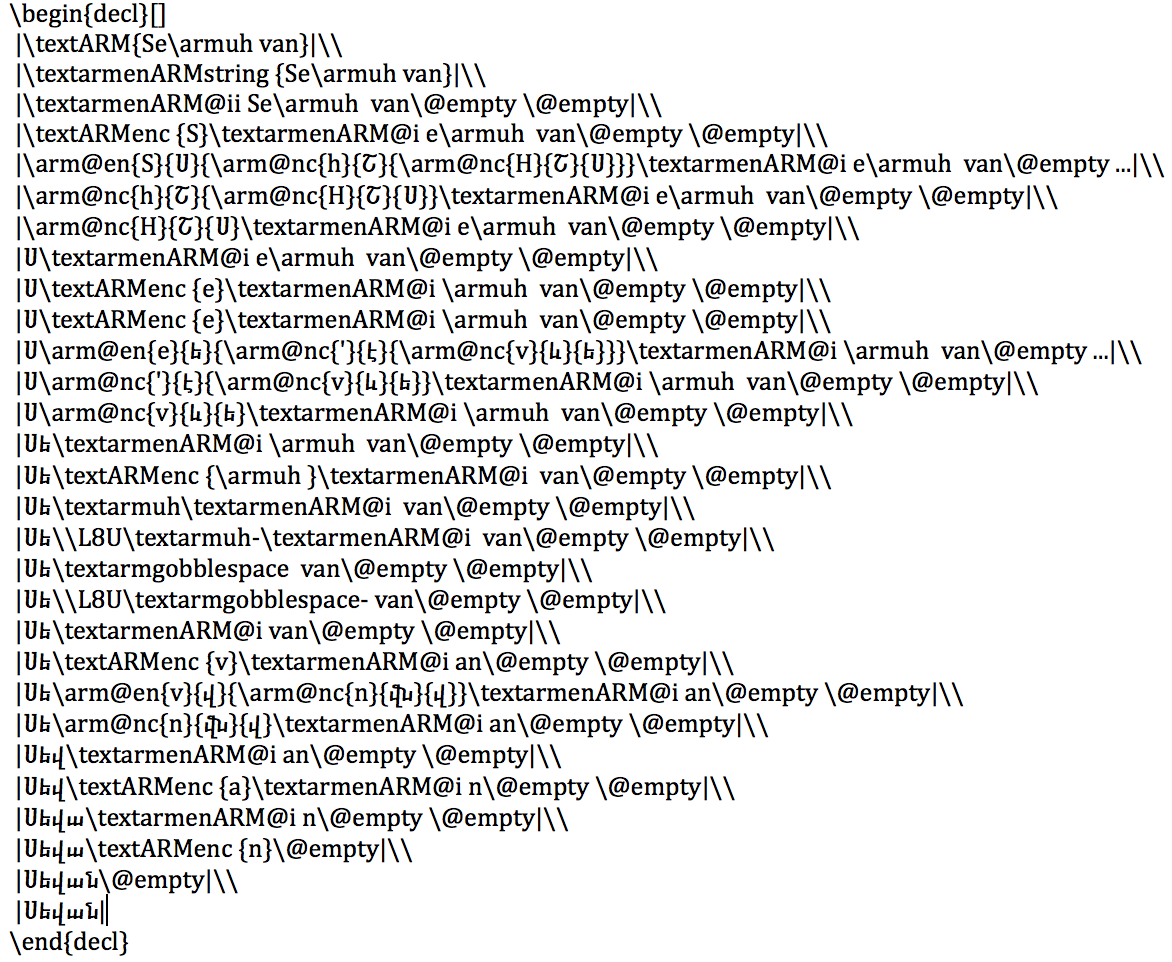
\includegraphics[scale=.625]{Armenian-example-UTF8.png}
%  \caption{Image of part of the source coding for Figure~\ref{ex-arm}, 
%  viewed as UTF-8 encoded, within editing software.}\label{src-arm}
% \end{figure}
%
% Several other `rebinding' commands are defined, mostly with package-loading options.
%\begin{itemize}
% \item |\LIIXUmapTeXnames| always defined
% \item |\LIIXUscriptcommands| handles |\textsuperscript|, |\textsubscript|, |\t|
% \item |\LIIXUtipacommands| handles IPA letters and symbols
% \item |\LIIXUmaparabicletters| with |arbxmp|
% \item |\LIIXUmaparmenianletters| with |armxmp| and |AR8xmp|
% \item |\LIIXUmapdevaccents| with |devxmp|
% \item |\LIIXUmapgreekletters| with |grkxmp| and |LGRxmp|
% \item |\LIIXUmaphebrewletters| with |hebxmp| and |HEBxmp|
% \item |\LIIXUmaplatinchars| and |\LIIXUcancelfontswitches| with |LATxmp|
% \item |\LIIXUmapmathletterlikes| always defined
% \item |\LIIXUmapmathspaces| always defined
% \item |\LIIXUmapmath...| with |mathxmp| --- see Section~\ref{ssec-math} below. 
%\end{itemize}
% It may well be that more macro names can be added to some of these commands,
% to allow macro usage within the metadata. 
% Suggestions for such additions should be sent to the |pdfx| package authors, along
% with example documents. Similarly support for more languages can be requested.
%
% \subsection[Nested Parsing\,\textemdash\,Mathematics in Metadata]%
%  {Nested Parsing\,\textemdash\,Mathematics in Metadata}\label{ssec-math}
%
% Macro commands for many mathematical symbols can be used directly in metadata without extra
% support; e.g., basic arithmetic operations, letter-like symbols, spacing commands.
% Super- and subscripted letters and numerals can use |\textsuperscript| and |\textsubscript|
% when there is an appropriate Unicode character (digits, comma, $+$/$-$/$=$, parentheses, 
% many letters but not all).
% 
% When the |mathxmp| loading option is specified, many more symbols become available,
% using `rebinding' macros. These are necessary, as the macros for mathematical symbols
% are generally \emph{not} defined as LICRs, but use |\mathchar|. Thus new LICRs are needed,
% and existing names bound to these.
%\begin{decl}[]
% |\LIIXUmapmathaccents| using `combining' characters from Unicode ranges at |Ux0300|, |Ux1DC0|, |Ux20D0|\\
% |\LIIXUmapisomathgreek| using |Ux0391|--|Ux03F8| for greek symbols\\
% |\LIIXUmapmatharrowsA| supporting symbols in the |Ux2190|--|Ux21FF| block\\
% |\LIIXUmapmathoperatorsA| supporting symbols in the |Ux2200|--|Ux227F| block\\
% |\LIIXUmapmathoperatorsB| supporting symbols in the |Ux2280|--|Ux22FF| block\\
% |\LIIXUmapmiscmathsymbolsA| supporting some symbols in the |Ux27C0|--|Ux27EF| range\\
% |\LIIXUmapsupparrowsA| supporting some symbols in the |Ux27F0|--|Ux27FF| block\\
% |\LIIXUmapsupparrowsB| supporting some symbols in the |Ux2900|-–|Ux297F| block\\
% |\LIIXUmapmiscmathsymbolsB| supporting symbols in the |Ux2980|--|Ux29FF| block\\
% |\LIIXUmapsuppmathoperators| supporting symbols in the |Ux2A00|--|Ux2AFF| block\\
% |\LIIXUmapunimathgreek| using |Ux1D6E2|--|Ux1D71B| for greek symbols\\
% |\LIIXUmapmathalphabets| allows access to symbols in the |Ux1D400|--|Ux1D755| block
%\end{decl}
%
% The `parser' macro idea can extends to handle a large class of mathematical expressions.
%\begin{decl}[]
% |\let\(\textinlinemath|\\
% |\DeclareTextCommand{\textinlinemath}{L8U}{\liixu@getinlinemath}|\\
% |\def\liixu@getinlinemath#1\){\space\textmathnormalstring{#1}\space}|\\
% |\DeclareTextCommand{\textmathnormalstring}{L8U}[1]{\textmathnormal@ii#1\@empty\@empty}|\\
% |\textmathnormal@ii #1#2\@empty -> ... |  coding to test what is in |#2|\\
% | ...  \textmathnormal{#1}\@empty | \quad if |#2| is |\@empty|\\
% | ...  \textmathnormal{#1}\textmathnormal@i #2\@empty | \quad if |#2| has more tokens\\
% |\let\[\textdisplaymath| defined similarly to call |\textmathnormalstring|
%\end{decl}
% This allows |\textmathnormal| to test each token, in particular mapping letters A--Za--z
% into the Unicode range |Ux1D44E|--|Ux1D467| (except for $h$).
% Mathematical styles, such as |\mathrm|, |\mathbf|, |\mathbb| etc. can now be handled
% using declarations such as:
%\begin{decl}[]
% |\Dec...positeCommand{\textmathnormal}{L8U}{\mathrm}{\liixu@mathreorder\textmathrmstring}|\\
% |\Dec...positeCommand{\textmathnormal}{L8U}{\mathbf}{\liixu@mathreorder\textmathbfstring}|\\
%\end{decl}
% where |\liixu@mathreorder| uses some \TeX\ pattern-matching to allow the |\textmathrmstring|
% parser macro to work on the argument to |\mathrm| before allowing |\textmathnormal| parsing
% to continue afterwards. We refer to this as `nested parsing'.
% 
% Similarly `nested parsing' can be used with superscripts and subscripts using |^{...}| and |_{...}| 
% and to specify linebreaks, and even super-/subscripts within styles; viz.
%\begin{decl}[]
% |\Declar...CompositeCommand{\textmathnormal}{L8U}{^}{\liixu@mathreorder\textsuperstring}|\\
% |\DeclareTextCompositeCommand{\textmathnormal}{L8U}{_}{\liixu@mathreorder\textsubstring}|\\
% |\DeclareTextCompositeCommand{\textmathnormal}{L8U}{\\}{\textLF}|\\
% |\DeclareTextCompositeCommand{\textmathnormal}{L8U}{\cr}{\textLF}|\\
% |\DeclareTextCompositeCommand{\textmathrm}{L8U}{^}{\liixu@mathreorder\textsuperstring}|\\
% |\DeclareTextCompositeCommand{\textmathrm}{L8U}{_}{\liixu@mathreorder\textsubstring}|
%\end{decl}
% Such `nested parsing' seems to be quite robust\footnote{%
% ... so far, barring multi-line aligned environments.}, but a great deal more testing
% is required to uncover cases which may require special handling.
% An ultimate aim is to be able to just copy the \LaTeX\ source for the `Abstract' of a technical
% paper into the |\Subject{...}| field of the |.xmpdata| file, with a large expectation that
% it will `just work', or need only trivial edits to make it so. 
%
%
% \subsection[Metadata in a Production Workflow]{Metadata in a Production Workflow}\label{ssec-wflow}
%
%\begin{figure}[htbp]
% \centering
% 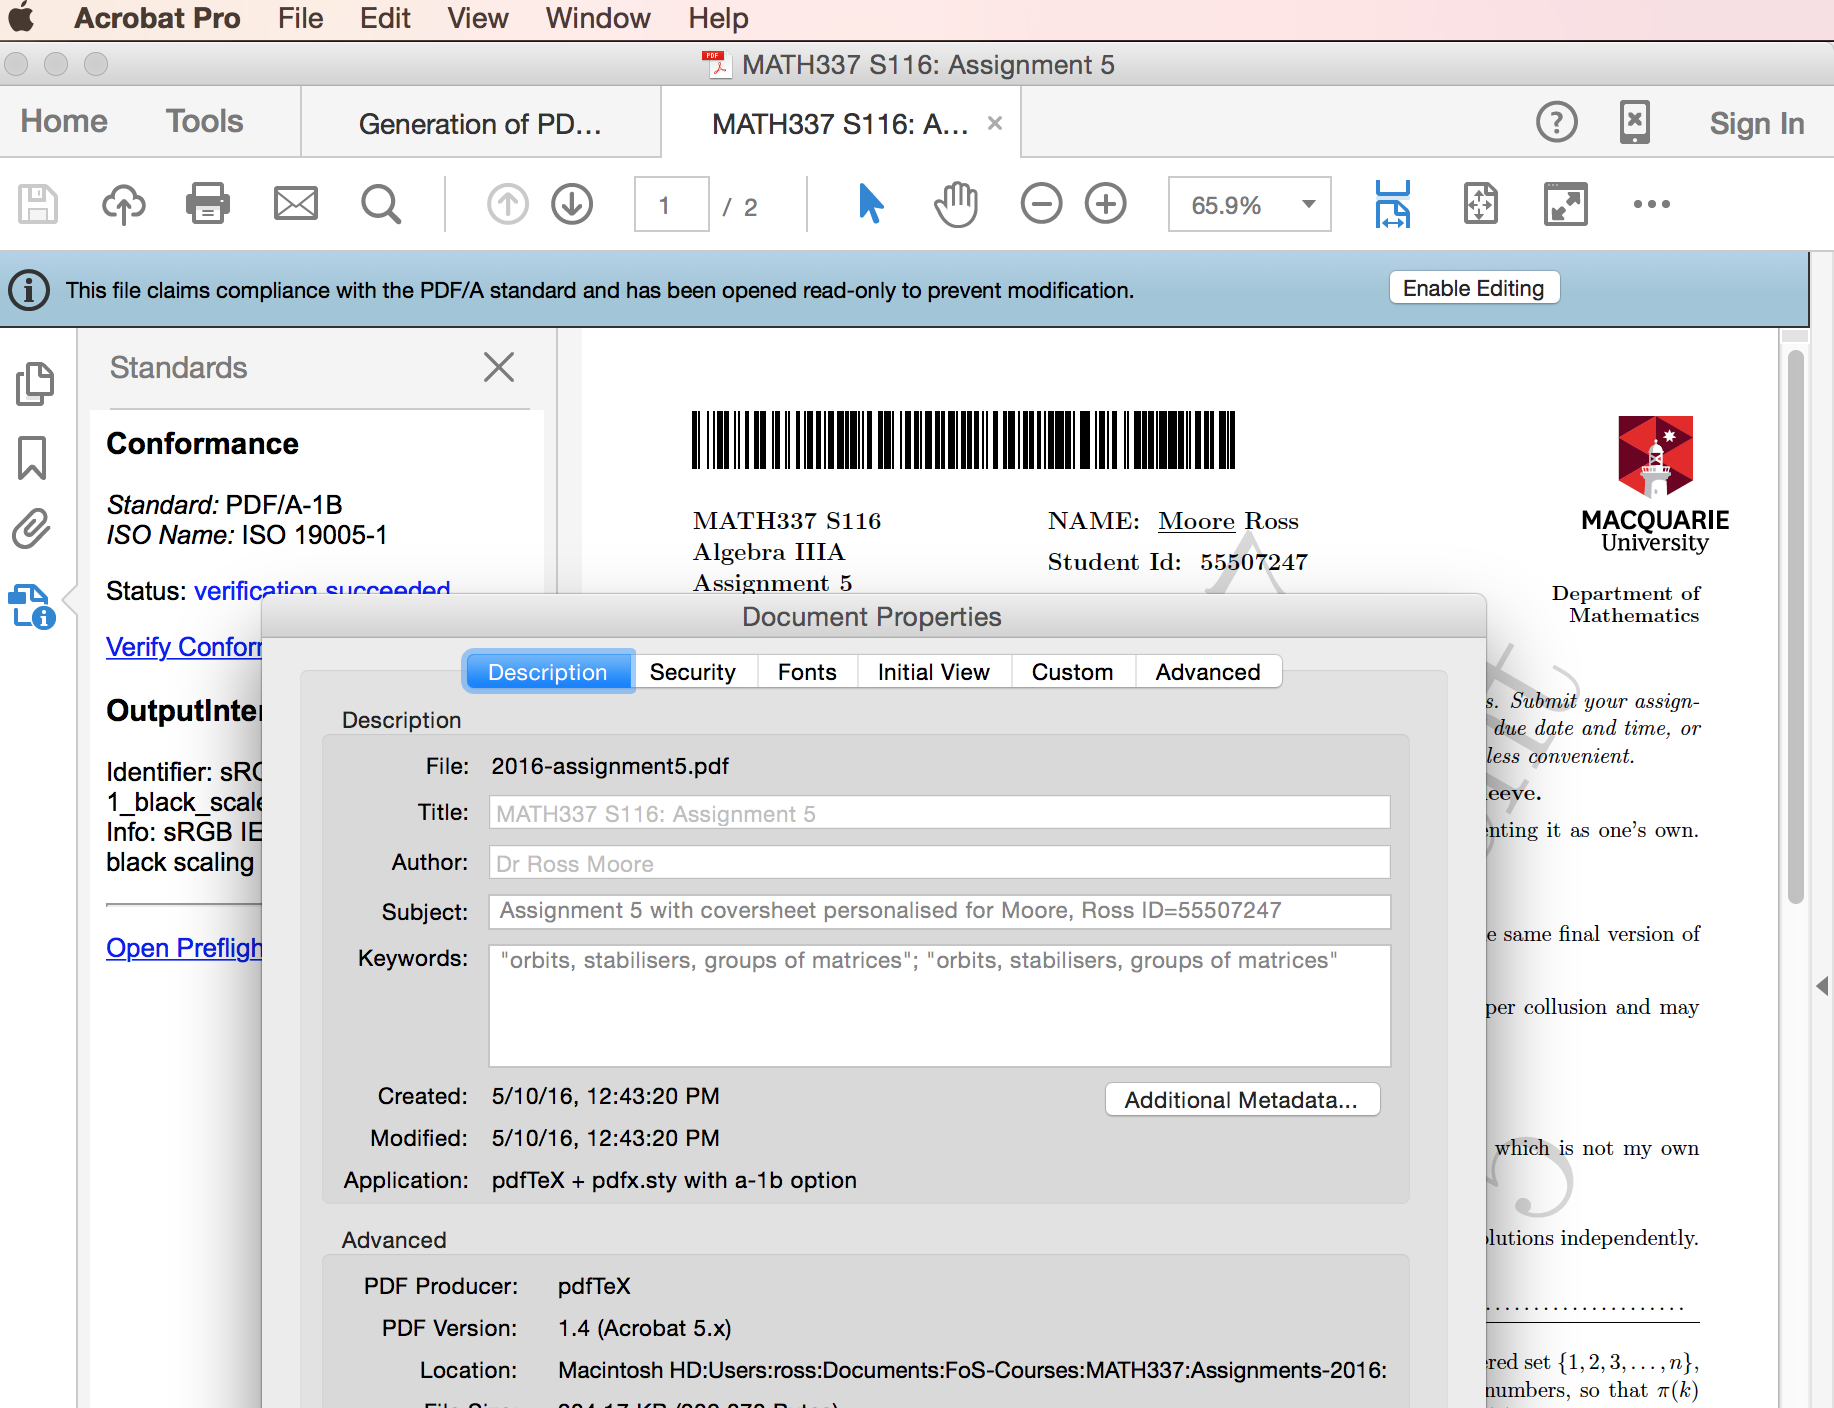
\includegraphics[scale=.45]{math-assign5.png}
% \caption{Metadata from student assignment papers, using information drawn from a database.
% The start of the \LaTeX\ coding for this example is shown in Figure~\ref{math-wflow}.}\label{wflow-meta}
%\end{figure}
% \noindent
% At Macquarie University, the Mathematics Department produces personalised topmatter
% or coversheets for student assignments and tutorial papers using \LaTeX, incorporating
% information that has been stored in a database. This is done by writing extra definitions 
% at the top of a copy of the \LaTeX\ source as prepared by the lecturers. 
% For example information analogous to the following
%\begin{decl}[]
% |\def\thestudentname{\utext{Moore} Ross}|\\
% |\def\thestudentid{55507247}|\\
% |\def\theunitcode{MATH337}|\\
% |\def\theoffering{S116}|\\
% |\def\thetaskname{Assignment 5}|\\
% |\def\theassignmentnumber{5}|\\
% |\def\theduedate{09/05 2016}|\\
% |...|
%\end{decl}
% is prepended to the file shown in Figure~\ref{math-wflow}, 
% for each student downloading their personalised assignment paper.
% The \LaTeX\ source makes use of this information, including recording some of it
% within the Metadata.
%\begin{figure}[!htbp]
%\begin{decl}[]
% |\providecommand{\theassignmentnumber}{5}|\\
% |\providecommand{\assignLecturer}{Dr Ross Moore}|\\
% |\providecommand{\theunitcode}{MATH337}|\\
% |\providecommand{\theunitname}{Algebra IIIA}|\\
% |\providecommand{\theyear}{2016}|\\
% |...|\\
% |\def\assigntopics{orbits, stabilisers, groups of matrices}|\\
% |\providecommand{\pdfxopts}{a-1b}|\\
% |%% XMP metadata for PDF/A conformance|\\
% |\begin{filecontents*}{\jobname.xmpdata}|\\
% |\Title{\theunitcode\ \theoffering: Assignment \theassignmentnumber}|\\
% |\Author{\assignLecturer}|\\
% |\Copyright{Macquarie University, Mathematics Department}|\\
% |\Subject{Assignment \theassignmentnumber, with coversheet personalised for \thestudentname,|\\
% |    id = \thestudentid}|\\
% |\Keywords{\assigntopics}|\\
% |\Creator{pdfTeX + pdfx.sty with \pdfxopts\space option}|\\
% |\pdfxEnableCommands{\def\utext#1{#1,}}|\\
% |\end{filecontents*}|\\
% ||\\
% |\documentclass[a4paper,11pt]{article}|\\
% |\RequirePackage{assignments}|\\
% |\usepackage[\pdfxopts]{pdfx}|
%\end{decl}
% \caption{Start of the \LaTeX\ source for an assignment paper, using macro expansion values
%  supplied via definitions prepended to this file.}\label{math-wflow}
%\end{figure}
% When preparing such documents \LaTeX's |\providecommand| is used to supply default values,
% not drawn from the database; but when actually used, these are ignored as the required
% information has been supplied using \TeX's |\def| command.
% The resulting metadata is as in Figure~\ref{wflow-meta}, showing also how the information
% is displayed at the top of the PDF file that is produced.
% Notice how a command |\utext| is included to obtain the underlining of the surname within
% the produced PDF. This is modified, using |\pdfxEnableCommands| in the |\jobname.xmpdata|
% file, to just place a comma after the surname in the metadata, as it precedes the given name.
%
%\newpage\noindent
% Another way that jobs can be customised using essentially the same \LaTeX\ source,
% is via the command used to initiate the job. For example the file |sample.tex|,
% accompanying the |pdfx| distribution, can be used to test the loading options to create
% PDFs conforming to the various flavours of PDF/A, PDF/E and PDF/X. 
% Consider a shell script containing the following (Unix/Linux) commands.
%\begin{decl}[]
% |pdflatex "\def\pdfxopt{a-2b}\input sample.tex"|\\
% |pdflatex "\def\pdfxopt{a-2b}\input sample.tex"|\\
% |mv sample.pdf sample-a2b.pdf|\\
% ||\\
% |pdflatex "\def\pdfxopt{a-2u}\input sample.tex"|\\
% |pdflatex "\def\pdfxopt{a-2u}\input sample.tex"|\\
% |mv sample.pdf sample-a2u.pdf|\\
% |...|
%\end{decl}
% With a 3-line block for each flavour, this produces a corresponding PDF
% from the same \LaTeX\ source, named according to each particular variant.
% A default |\providecommand{\pdfxopt}{a-1b}| at the start of |sample.tex| catches the case
% of normal typesetting, doing nothing when |\pdfxopt| already has an expansion value.
% 
% \goodbreak
% \subsection[Further Developments]{Further Developments}\label{ssec-further}
%
% Prospects for further development of the |pdfx| package are as follows, 
% listed not necessarily in order of perceived importance.
% \begin{itemize}
%  \item
%    Support for the |dvips| driver with Ghostscript as PDF producer; possible since |gs v9.21|.
%  \item
%    Separate the |L8U| pseudo-encoding support into a separate package.
%  \item
%    Conformance to multiple PDF standards; e.g. both PDF/A and PDF/E,
%     both PDF/A and PDF/X with RGB or CMYK color profile, other combinations.
%  \item
%    Explore delaying the processing of metadata until |\begin{document}|, 
%    thereby allowing some fields to be set automatically from other information
%    supplied within the document preamble.
%  \item
%    Support for input using other legacy 8-bit encodings and transliterations.
%  \item
%    Support for more mathematical environments within the metadata.
%  \item
%    Support for more PRISM metadata fields, incl. PRISM 3.0~\cite{PRISM}.
%  \item
%    Explore ways to overcome incompatibilities that may arise with other packages.
%  \item
%    Full support for PDF/VT; in particular, transparency groups and PDF/VT-2s.
%  \item
%    Support for more aspects of PDF/UA and `Tagged PDF'.
%  \item
%    Develop ways to usefully use |L8U| apart from metadata and bookmarks.
%  \item
%   Support emerging standards based on PDF 2.0~\cite{PDF20}.
% \end{itemize}
%
%
% \section[Bibliography]{Bibliography}%
% {\let\newpage\relax
% \begin{thebibliography}{999}
%
% \bibitem{PDF17}Adobe Systems Inc.;
% {PDF} Reference 1.7, November 2006.
% Also available as \cite{ISO32000}.\\
% \url{http://www.adobe.com/devnet/pdf/pdf_reference.html}.
%
% \bibitem{XMP-spec}Adobe Systems Inc.;
%  XMP Specification, Adding Intelligence to Media. September 2005.
% Also available as ISO 16684-1:2012\,\cite{XMP-ISO}.\\
% \url{http://www.adobe.com/devnet/xmp/}.
%
% \bibitem{PDFUA1} ANSI\,/\,AIIM\,/\,ISO\,14289-1:2012;
% Document management applications --- Electronic document file format enhancement for accessibility
% --- Part 1: Use of ISO\,32000-1\,(PDF/UA-1);
% Technical Committee ISO/TC\,171/SC\,2 (July 2012).
% \url{http://www.iso.org/iso/home/store/catalogue_tc/catalogue_detail.htm?csnumber=54564}.\\
% Revised as ISO\,14289-1:2014 (December 2014): 
% \url{http://www.iso.org/iso/home/store/catalogue_tc/catalogue_detail.htm?csnumber=64599}.\\
% Available from ANSI at \url{https://webstore.ansi.org/Standards/ISO/ISO142892014}.
%
% \bibitem{PDFUABSI} BS,/\,ISO\,14289-1:2014; Document Management Applications. 
% Electronic Document File Format Enhancement For Accessibility. Use Of ISO 32000-1 (PDF/UA-1) (British Standard)
% \url{https://webstore.ansi.org/Standards/BSI/BSISO142892014}.
%
%  \bibitem{pdfaPilot} Callas Software Gmbh.; 
%  \texttt{pdfaPilot}, plug-in or desktop software for PDF/A versions.
%  \url{https://www.callassoftware.com/en/products/pdfapilot}.
%
% \bibitem{DC}
% Dublin Core Metadata Element Set, Version 1.1, October 2010\\ 
% \url{http://dublincore.org/documents/dces/}.
%
% \bibitem{BCP47}IETF; Best Current Practice \#47: Tags for Identifying Languages.
% Incorporates RFC\,5646; obsoletes RFC\,4646. IETF Network Working Group, September 2009.
%  \url{https://tools.ietf.org/pdf/bcp47.pdf}.
%
% \bibitem{PDFX}ISO\,15930-1:2001;
% Graphic technology --- Prepress digital data exchange --- Use of PDF --- Part 1: 
% Complete exchange using CMYK data (PDF/X-1 and PDF/X-1a).
% Technical Committee ISO/TC\,130 (December 2001).
% \url{http://www.iso.org/iso/home/store/catalogue_tc/catalogue_detail.htm?csnumber=29061}.
%
% \bibitem{PDFX3}ISO\,15930-3:2002;
% Graphic technology --- Prepress digital data exchange --- Use of PDF --- Part 3: 
% Complete exchange suitable for colour-managed workflows (PDF/X-3).
% Technical Committee ISO/TC\,130 (September 2002).
% \url{http://www.iso.org/iso/home/store/catalogue_tc/catalogue_detail.htm?csnumber=34941}.
%
% \bibitem{PDFX1a}ISO\,15930-4:2003;
% Graphic technology --- Prepress digital data exchange --- Use of PDF --- Part 4: 
% Complete exchange of CMYK and spot colour printing data using PDF 1.4 (PDF/X-1a).
% Technical Committee ISO/TC\,130 (December 2003).
% \url{http://www.iso.org/iso/home/store/catalogue_tc/catalogue_detail.htm?csnumber=39938}.
%
% \bibitem{PDFX3a}ISO\,15930-6:2003;
% Graphic technology --- Prepress digital data exchange --- Use of PDF --- Part 6: 
% Complete exchange of printing data suitable for colour-managed workflows using PDF 1.4 (PDF/X-3).
% Technical Committee ISO/TC\,130 (December 2003).
% \url{http://www.iso.org/iso/home/store/catalogue_tc/catalogue_detail.htm?csnumber=39940}.
%
% \bibitem{PDFX4}ISO\,15930-7:2010;
% Graphic technology --- Prepress digital data exchange --- Use of PDF --- Part 7: 
% Complete exchange of printing data (PDF/X-4) and partial exchange of printing data with external profile reference (PDF/X-4p) using PDF 1.6.
% Technical Committee ISO/TC\,130 (July 2010).
% \url{http://www.iso.org/iso/home/store/catalogue_tc/catalogue_detail.htm?csnumber=55843}.
%
% \bibitem{PDFX5}ISO\,15930-8:2010;
% Graphic technology --- Prepress digital data exchange --- Use of PDF --- Part 8: 
% Partial exchange of printing data using PDF 1.6 (PDF/X-5). \hfil
% Technical Committee ISO/TC\,130 (July 2010). \hfil
% \url{http://www.iso.org/iso/home/store/catalogue_tc/catalogue_detail.htm?csnumber=55844}.
% Revision via Corrigendum: ISO\,15930-8:2010/Cor\,1:2011 (August 2011);
% \url{http://www.iso.org/iso/home/store/catalogue_tc/catalogue_detail.htm?csnumber=60210}.
%
% \bibitem{PDFVT}ISO\,16612-2:2010;
% Graphic technology\,---\,Variable data exchange\,---\,Part 2:\hfil
% Using PDF/X-4 \penalty-5000 and PDF/X-5 (PDF/VT-1 and PDF/VT-2).
% Technical Committee ISO/TC\,130 (December 2005). \hfil
% \href{http://www.iso.org/iso/home/store/catalogue_tc/catalogue_detail.htm?csnumber=38013}%
%  {{\small\tt http://www.iso.org/iso/home/store/catalogue\_tc/catalogue\_detail.htm?\penalty-200csnumber=38013}}.
%
% \bibitem{XMP-ISO}ISO\,16684-1:2012;
% Graphic technology --- Extensible metadata platform (XMP) specification --- Part 1: 
% Data model, serialization and core properties.
% Technical Committee ISO/TC\,130 (February 2012).
% \url{http://www.iso.org/iso/home/store/catalogue_tc/catalogue_detail.htm?csnumber=57421}.
%
% \bibitem{PDFA}ISO\,19005-1:2005; 
% Document Management --- Electronic document file format for long term preservation
% --- Part 1: Use of PDF\,1.4\,(PDF/A-1);
% Technical Committee ISO/TC\,171/SC\,2  (Sept. 2005).
% Revisions via Corrigenda: ISO\,19005-1:2005/Cor\,1:2007 (March 2007); 
% ISO\,19005-1:2005/Cor\,2:2011 (Dec. 2011). \\
% \url{http://www.iso.org/iso/catalogue_detail?csnumber=38920}.
%
% \bibitem{PDFA2}ISO\,19005-2:2011;
% Document Management --- Electronic document file format for long term preservation
% --- Part 2: Use of ISO\,32000-1\,(PDF/A-2); \hfill
% Technical Committee ISO/\penalty-200 TC\,171/SC\,2 (June 2011).\\
% \url{http://www.iso.org/iso/catalogue_detail?csnumber=50655}. 
%
% \bibitem{PDFA3}ISO\,19005-3:2012;
% Document Management --- Electronic document file format for long term preservation
% --- Part 3: Use of ISO\,32000-1 with support for embedded files (PDF/A-3);
% Technical Committee ISO/TC\,171/SC\,2 (October 2012).\\
% \url{http://www.iso.org/iso/catalogue_detail?csnumber=57229}. 
%
% \bibitem{PDFE}ISO\,24517-1:2008;
% Document Management --- Engineering document format using PDF --- Part 1: 
% Use of PDF 1.6 (PDF/E-1);
% Technical Committee ISO/TC\,171/SC\,2 (May 2008).\\
% \url{http://www.iso.org/iso/catalogue_detail?csnumber=42274}. 
%
% \bibitem{ISO32000}ISO\,32000-1:2008;
% Document management\,---\,Portable document format\,(PDF\,1.7);
% Technical Committee ISO/TC\,171/SC\,2 (July 2008). 
% Also available as \cite{PDF17}.\\
% \url{http://www.iso.org/iso/catalogue_detail?csnumber=51502}.
%
% \bibitem{PDF20}ISO\,32000-2:2017;
% Document management --- Portable document format --- Part~2: PDF\,2.0;
% Technical Committee ISO/TC\,171/SC\,2 Document file formats, EDMS systems 
% and authenticity of information. (July 2017)\\
% \url{https://www.iso.org/standard/63534.html}.
%
% \bibitem{LC2} F.\,Mittelbach, M.\,Goossens with J.\,Braams, D.\,Carlisle, C.\,Rowley;
% The \LaTeX\ Companion --- 2nd edition. Addison--Wesley (now Pearson Education Inc.), 2004.
% ISBN 0-201-36299-6 (paperback).
%
% \bibitem{TN0009}PDF/A Competence Centre;
% TechNote 0009: XMP Extension Schemas in PDF/A-1. (March 2008)
% \href{https://www.pdfa.org/publication/technical-note-tn-0009-xmp-extension-schemas-in-pdfa-1/}%
% {\small\tt https://www.pdfa.org/publication/technical-note-tn-0009-xmp-extension\penalty-200 -schemas-in-pdfa-1/}.
%
% \bibitem{PDF-UA}
% PDF/UA Technical Implementation Guide: Understanding ISO\,14289-1 (PDF/UA-1). \penalty-200
% AIIM Global Community of Information Professionals. \hfil
% \href{http://www.aiim.org/Research-and-Publications/standards/committees/PDFUA/Technical-Implementation-Guide}%
% {\small\tt http://www.aiim.org/Re\penalty-200 search-and-Publications/standards/committees/PDFUA/Technical-Implementation\penalty-200 -Guide}.
%
% \bibitem{colorp} N.\,Preining; 
% \texttt{colorprofiles} \textemdash\ Collection of free ICC profiles.
%  \TeX\ and \LaTeX\ package (by R.\,Moore), distributed with \TeX{}Live. (November 2018)\\
%  \url{https://ctan.org/pkg/colorprofiles}.
%
% \bibitem{PRISM}PRISM; Publishing Requirements for Industry Standard Metadata. 
%  PRISM Metadata Initiative; Idealliance Working Group.
% \url{http://www.idealliance.org/specifications/prism-metadata-initiative/prism}
%
% \bibitem{pdfx}C.\,V.\,Radhakrishnan, \Thanh, Ross Moore, Peter Selinger;
% Generation of PDF/X- and PDF/A-compliant PDFs with \pdftex --- \texttt{pdfx.sty}.
% TUGboat Vol.\,36, No.\,2; TUG 2015 Conference Proceedings. \TeX\ Users Group, 2015; pp.\,136--142.
%
% \bibitem{veraPDF} veraPDF. Industry Supported PDF/A Validation. 
% Software, dual-licensed under the GNU General Public License v3 or later (GPLv3+) 
% and Mozilla Public License v2 or later (MPLv2+). \url{https://verapdf.org}.
% Wiki: \url{https://github.com/veraPDF/veraPDF-validation-profiles/wiki}
%
% \bibitem{RDF} World Wide Web Consortium (W3C); 
% Resource Description Format: RDF 1.1 XML Syntax. W3C Recommendation. (February 2014)
% \url{https://www.w3.org/TR/rdf-syntax-grammar/}.
% 
% \bibitem{wikiPDF}Wikipedia; 
% PDF/A: \url{https://en.wikipedia.org/wiki/PDF/A}\newline
% PDF/E: \url{https://en.wikipedia.org/wiki/PDF/E}\newline
% PDF/VT: \url{https://en.wikipedia.org/wiki/PDF/VT}\newline
% PDF/UA: \url{https://en.wikipedia.org/wiki/PDF/UA}\newline
% PDF/X: \url{https://en.wikipedia.org/wiki/PDF/X}
%
% \end{thebibliography}
% }\goodbreak
% \section[Implementation]{Implementation}
% 
% \iffalse
%<*package>
% \fi \hfuzz=2.5pt%
%    \begin{macrocode}
\@ifpackageloaded{pdfxmult}{%
 \PackageError{pdfx}%
  {^^JThis package may not be used in conjunction with the \space
   pdfxmult \space package}%
  {Type \space x <return> \space to exit; or just \space <return> \space
   to continue without this package.}%
 \expandafter\let\csname opt@pdfx.sty\endcsname\@empty\endinput
}{}%
\NeedsTeXFormat{LaTeX2e}
\ProvidesPackage{pdfx}
  [2019/02/27 v1.6.3 PDF/X and PDF/A support (CVR/HTH/RRM/PS)]

\newif\ifpdfx@noBOM \pdfx@noBOMfalse   % use a BOM in the XMP packet
\newif\ifpdfx@x \pdfx@xfalse   % PDF/X mode
\newif\ifpdfx@e \pdfx@efalse   % PDF/E mode; not fully implemented yet
\newif\ifpdfx@ua\pdfx@uafalse   % PDF/UA mode; not fully implemented yet
\newif\ifpdfx@vt \pdfx@vtfalse   % PDF/VT mode, extension of  PDF/X
\newif\ifno@iccprofile   % used with PDF/X-4p and PDF/X-5pg
\newif\ifpdfx@noerr   % error messages become just warnings
\newif\ifpdfx@omitcharset % used with  pdfomitcharset  primitive

\DeclareOption{noerr}{\pdfx@noerrtrue}

%% Not all combinations of the following parameters are meaningful.
\def\xmp@Part{1}               % PDF/A part: 1, 2, or 3
\def\xmp@Conformance{B}        % Conformance level: A, B, or U
\def\xmp@ReleaseDate{2005}     % 2001 for PDF/X-1, 2005 for PDF/A-1,
                               % 2010 for PDF/A-2, 2012 for PDF/A-3.

\newcount\pdfx@minorversion
\expandafter\ifx\csname pdfminorversion\endcsname\relax
\else
 \global\pdfx@minorversion=\the\pdfminorversion
\fi

\def\pdfx@ErrorWarning#1#2#3#4{%
 \ifpdfx@noerr \PackageWarning{pdfx}{#1.^^J  #2#3.^^J}%
 \else \PackageError{pdfx}{#1}{#2#4.^^J
    Use option 'noerr' to avoid this message.^^J}%
 \fi}

\def\pdfx@Xvn@message{%
 \pdfx@ErrorWarning{PDF/X-5n has no default profile}%
   {Provide your own}{; continuing to build a non-valid document}%
   {, else continue to build a non-valid document}%
}

%%  support  pdfomitcharset  primitive, added to pdfTeX in 2019
\DeclareOption{nocharset}{\pdfx@omitcharsettrue}
\DeclareOption{usecharset}{\pdfx@omitcharsetfalse}

%% PDF/A options
%%  default is to create  PDF/A-1b
%%  options can change this for PDF/X or higher levels of PDF/A
\DeclareOption{a-1a}{\global\pdfx@xfalse\def\xmp@Part{1}%
 \def\xmp@Conformance{A}\def\xmp@ReleaseDate{2005}%
 \pdfx@omitcharsetfalse}
\DeclareOption{a-1b}{\global\pdfx@xfalse\def\xmp@Part{1}%
 \def\xmp@Conformance{B}\def\xmp@ReleaseDate{2005}%
 \pdfx@omitcharsetfalse}
\DeclareOption{a-2a}{\global\pdfx@xfalse\def\xmp@Part{2}%
 \def\xmp@Conformance{A}\def\xmp@ReleaseDate{2010}%
 \pdfx@omitcharsettrue}
\DeclareOption{a-2b}{\global\pdfx@xfalse\def\xmp@Part{2}%
 \def\xmp@Conformance{B}\def\xmp@ReleaseDate{2010}%
 \pdfx@omitcharsettrue}
\DeclareOption{a-2u}{\global\pdfx@xfalse\def\xmp@Part{2}%
 \def\xmp@Conformance{U}\def\xmp@ReleaseDate{2010}%
 \pdfx@omitcharsettrue}
\DeclareOption{a-3a}{\global\pdfx@xfalse\def\xmp@Part{3}%
 \def\xmp@Conformance{A}\def\xmp@ReleaseDate{2012}%
 \pdfx@omitcharsettrue}
\DeclareOption{a-3b}{\global\pdfx@xfalse\def\xmp@Part{3}%
 \def\xmp@Conformance{B}\def\xmp@ReleaseDate{2012}%
 \pdfx@omitcharsettrue}
\DeclareOption{a-3u}{\global\pdfx@xfalse\def\xmp@Part{3}%
 \def\xmp@Conformance{U}\def\xmp@ReleaseDate{2012}%
 \pdfx@omitcharsettrue}
%%
%% PDF/X options
%% comments added, using
%% https://www.eci.org/_media/downloads/pdfx/pdfx_faq_english_nov05.pdf
%% https://en.wikipedia.org/wiki/PDF/X#List_of_the_PDF.2FX_standards
%%
\DeclareOption{x-1}{\global\pdfx@xtrue\def\xmp@Part{1}%  obsolete
 \def\xmp@Conformance{a}\def\xmp@ReleaseDate{1999}% CMYK only
 \global\pdfx@minorversion=2\relax
 \pdfx@ErrorWarning{PDF/X-1:1999 is no longer an accepted standard}%
    {Use option  x-1a1 or  x-1a3 }{; continuing to build a non-valid document}%
    {, else continue to build a non-valid document.}%
 }%  effectively same as  x-1a1
\DeclareOption{x-1a}{\global\pdfx@xtrue\def\xmp@Part{1}% CMYK only
 \def\xmp@Conformance{a}\def\xmp@ReleaseDate{2003}%
 \global\pdfx@minorversion=3 }%  same as  x-1a3
\DeclareOption{x-1a1}{\global\pdfx@xtrue\def\xmp@Part{1}%
 \def\xmp@Conformance{a}\def\xmp@ReleaseDate{2001}%  ISO 15930-1:2001
 \global\pdfx@minorversion=3 }
\DeclareOption{x-1a3}{\global\pdfx@xtrue\def\xmp@Part{1}%
 \def\xmp@Conformance{a}\def\xmp@ReleaseDate{2003}%  ISO 15930-4:2003
 \global\pdfx@minorversion=3 }
\DeclareOption{x-2}{\global\pdfx@xtrue\def\xmp@Part{2}%  XMP Metadata
%% \def\xmp@Conformance{}\def\xmp@ReleaseDate{2002}%  ISO 15930-2:2003
 \def\xmp@Conformance{}\def\xmp@ReleaseDate{2003}%   ISO 15930-5, withdrawn 2011
 \global\pdfx@minorversion=4\relax
 \pdfx@ErrorWarning{PDF/X-2:2003 was never published as a standard}%
   {Use option  x-1a or  x-3 }{; continuing to build a non-valid document}%
   {, else continue to build a non-valid document}%
 }%  external OPI workflow, i.e. multiple files involved
\DeclareOption{x-3}{\global\pdfx@xtrue\def\xmp@Part{3}% RGB allowed, but rare!
 \def\xmp@Conformance{}\def\xmp@ReleaseDate{2003}%
 \global\pdfx@minorversion=4 }%  same as x-303
\DeclareOption{x-302}{\global\pdfx@xtrue\def\xmp@Part{3}%
 \def\xmp@Conformance{}\def\xmp@ReleaseDate{2002}%   ISO 15930-3:2002
 \global\pdfx@minorversion=3 }
\DeclareOption{x-303}{\global\pdfx@xtrue\def\xmp@Part{3}%
 \def\xmp@Conformance{}\def\xmp@ReleaseDate{2003}%  ISO 15930-6:2003
 \global\pdfx@minorversion=4 }
%%%  Later versions, yet to be fully implemented
\DeclareOption{x-4}{\global\pdfx@xtrue\def\xmp@Part{4}%
 \def\xmp@Conformance{}\def\xmp@ReleaseDate{2010}%  ISO 15930-7:2010
 \global\pdfx@minorversion=6 }%  same as  x-410
\DeclareOption{x-4p}{\global\pdfx@xtrue\global\no@iccprofiletrue
  \def\xmp@Part{4}\def\xmp@Conformance{p}\def\xmp@ReleaseDate{2010}%
  \global\pdfx@minorversion=6 }%  same as  x-4p10
\DeclareOption{x-408}{\global\pdfx@xtrue\def\xmp@Part{4}%
 \def\xmp@Conformance{}\def\xmp@ReleaseDate{2008}%  ISO 15930-7:2008
 \global\pdfx@minorversion=6 }
\DeclareOption{x-410}{\global\pdfx@xtrue\def\xmp@Part{4}%
 \def\xmp@Conformance{}\def\xmp@ReleaseDate{2010}%  ISO 15930-7:2010
 \global\pdfx@minorversion=6 }
\DeclareOption{x-4p08}{\global\pdfx@xtrue\global\no@iccprofiletrue
  \def\xmp@Part{4}\def\xmp@Conformance{p}\def\xmp@ReleaseDate{2008}%
  \global\pdfx@minorversion=6 }%   ISO 15930-7:2010
\DeclareOption{x-4p10}{\global\pdfx@xtrue\global\no@iccprofiletrue
  \def\xmp@Part{4}\def\xmp@Conformance{p}\def\xmp@ReleaseDate{2010}%
  \global\pdfx@minorversion=6 }%   ISO 15930-7:2010
\DeclareOption{x-5}{\global\pdfx@xtrue\def\xmp@Part{5}%
 \def\xmp@Conformance{g}\def\xmp@ReleaseDate{2008}%
 \global\pdfx@minorversion=6 }%   ISO 15930-8:2010
\DeclareOption{x-5g}{\global\pdfx@xtrue\def\xmp@Part{5}%
 \def\xmp@Conformance{g}\def\xmp@ReleaseDate{2008}%
 \global\pdfx@minorversion=6 }%   ISO 15930-8:2010
\DeclareOption{x-5n}{\global\pdfx@xtrue %\global\no@iccprofiletrue
 \def\xmp@Part{5}\def\xmp@Conformance{n}\def\xmp@ReleaseDate{2010}%
 \global\pdfx@minorversion=6 \pdfx@Xvn@message}%   ISO 15930-8:2010
\DeclareOption{x-5pg}{\global\pdfx@xtrue\global\no@iccprofiletrue
  \def\xmp@Part{5}\def\xmp@Conformance{pg}\def\xmp@ReleaseDate{2010}%
  \global\pdfx@minorversion=6 }%  ISO 15930-8:2010
\DeclareOption{x-508}{\global\pdfx@xtrue\def\xmp@Part{5}%
 \def\xmp@Conformance{g}\def\xmp@ReleaseDate{2008}%
 \global\pdfx@minorversion=6 }%   ISO 15930-8:2008
\DeclareOption{x-5g08}{\global\pdfx@xtrue\def\xmp@Part{5}%
 \def\xmp@Conformance{g}\def\xmp@ReleaseDate{2008}%
 \global\pdfx@minorversion=6 }%   ISO 15930-8:2008
\DeclareOption{x-5n08}{\global\pdfx@xtrue %\global\no@iccprofiletrue
 \def\xmp@Part{5}\def\xmp@Conformance{n}\def\xmp@ReleaseDate{2008}%
 \global\pdfx@minorversion=6 \pdfx@Xvn@message}%   ISO 15930-8:2008
\DeclareOption{x-5pg08}{\global\pdfx@xtrue\global\no@iccprofiletrue
  \def\xmp@Part{5}\def\xmp@Conformance{pg}\def\xmp@ReleaseDate{2008}%
  \global\pdfx@minorversion=6 }%  ISO 15930-8:2008
\DeclareOption{x-510}{\global\pdfx@xtrue\def\xmp@Part{5}%
 \def\xmp@Conformance{g}\def\xmp@ReleaseDate{2010}%
 \global\pdfx@minorversion=6 }%  ISO 15930-8:2010
\DeclareOption{x-5g10}{\global\pdfx@xtrue\def\xmp@Part{5}%
 \def\xmp@Conformance{g}\def\xmp@ReleaseDate{2010}%
 \global\pdfx@minorversion=6 }%  ISO 15930-8:2010
\DeclareOption{x-5n10}{\global\pdfx@xtrue %\global\no@iccprofiletrue
 \def\xmp@Part{5}\def\xmp@Conformance{n}\def\xmp@ReleaseDate{2010}%
 \global\pdfx@minorversion=6 \pdfx@Xvn@message}%  ISO 15930-8:2010
\DeclareOption{x-5pg10}{\global\pdfx@xtrue\global\no@iccprofiletrue
  \def\xmp@Part{5}\def\xmp@Conformance{pg}\def\xmp@ReleaseDate{2010}%
  \global\pdfx@minorversion=6 }%  ISO 15930-8:2010
%%
%% PDF/E options
%%
\DeclareOption{e}{\global\pdfx@xfalse\global\pdfx@etrue
  \def\xmp@Part{1}\def\xmp@Conformance{}\def\xmp@ReleaseDate{2008}%
  \gdef\thepdfminorversion{6}%   same as  e-1
  }
\DeclareOption{e-1}{\global\pdfx@xfalse\global\pdfx@etrue
  \def\xmp@Part{1}\def\xmp@Conformance{}\def\xmp@ReleaseDate{2008}%
  \gdef\thepdfminorversion{6}%  ISO 24517-1:2008
  }
%% PDF/UA options
%%
\let\xmp@PDFUA\@empty
\DeclareOption{ua}{\global\pdfx@uatrue % ISO 14289-1:2012, 2014
  \def\xmp@UAlevel{1}\let\xmp@PDFUA\relax}%   same as  ua-1
\DeclareOption{ua-1}{\global\pdfx@uatrue % ISO 14289-1:2012, 2014
  \def\xmp@UAlevel{1}\let\xmp@PDFUA\relax}
%%
%% PDF/VT options
%%
\DeclareOption{vt-1}{\global\pdfx@xtrue\global\pdfx@vttrue
  \def\xmp@Part{4}\def\xmp@vtPart{1}\def\xmp@Conformance{}%
  \def\xmp@vtConformance{}\def\xmp@ReleaseDate{2010}%
  \gdef\xmpMM@VersionID{1}%
  \global\pdfx@minorversion=6 }
\DeclareOption{vt-2}{\global\pdfx@xtrue\global\pdfx@vttrue
  \global\no@iccprofiletrue   \gdef\xmpMM@VersionID{1}%
  \def\xmp@Part{5}\def\xmp@vtPart{2}\def\xmp@Conformance{pg}%
  \def\xmp@vtConformance{}\def\xmp@ReleaseDate{2010}%
  \global\pdfx@minorversion=6 }
\DeclareOption{vt-2s}{\global\pdfx@xtrue\global\pdfx@vttrue
  \global\no@iccprofiletrue   \gdef\xmpMM@VersionID{1}%
  \def\xmp@Part{5}\def\xmp@vtPart{2}\def\xmp@Conformance{pg}%
  \def\xmp@vtConformance{s}\def\xmp@ReleaseDate{2010}%
  \global\pdfx@minorversion=6 }

%% options to alter PDF minor version, in case needed in special circumstances
\DeclareOption{pdf12}{\global\pdfx@minorversion=2 }%  1999
\DeclareOption{pdf13}{\global\pdfx@minorversion=3 }%  2001  Acrobat 4 (ISBN 0-201-61588-6)
\DeclareOption{pdf14}{\global\pdfx@minorversion=4 }%  2003  Acrobat 5 (ISBN 0-201-75839-3)
\DeclareOption{pdf15}{\global\pdfx@minorversion=5 }%  2005  Acrobat 6
\DeclareOption{pdf16}{\global\pdfx@minorversion=6 }%  2006  Acrobat 7 (ISBN 0-321-30474-8)
\DeclareOption{pdf17}{\global\pdfx@minorversion=7 }%  2008  ISO 32000-1:2008

%% inhibits writing the XMP byte-order marker
\DeclareOption{noBOM}{\pdfx@noBOMtrue}
\DeclareOption{useBOM}{\pdfx@noBOMfalse}

%% options for language character macros in XMP metadata
\newif\ifcyrxmp
\newif\ifcyrKOIxmp
\newif\ifgrkxmp
\newif\ifgrkLGRxmp
\newif\ifhebxmp
\newif\ifhebHEBxmp
\newif\ifarbxmp
\newif\ifarmxmp
\newif\ifarmSCIxmp
\newif\ifdevxmp
\newif\ifvnmxmp
\newif\iflatEXTxmp
\newif\iflatLATxmp
\newif\ifipaxmp
\newif\ifmathxmp

\DeclareOption{latxmp}{\global\latEXTxmptrue}
\DeclareOption{LATxmp}{\global\latLATxmptrue\global\latEXTxmptrue}
\DeclareOption{cyrxmp}{\global\cyrxmptrue}
\DeclareOption{KOIxmp}{\global\cyrKOIxmptrue\global\cyrxmptrue}
\DeclareOption{grkxmp}{\global\grkxmptrue}
\DeclareOption{LGRxmp}{\global\grkLGRxmptrue\global\grkxmptrue}
\DeclareOption{hebxmp}{\global\hebxmptrue}
\DeclareOption{HEBxmp}{\global\hebHEBxmptrue\global\hebxmptrue}
\DeclareOption{arbxmp}{\global\arbxmptrue}
\DeclareOption{armxmp}{\global\armxmptrue}
\DeclareOption{AR8xmp}{\global\armSCIxmptrue\global\armxmptrue}
\DeclareOption{devxmp}{\global\devxmptrue}
\DeclareOption{vnmxmp}{\global\vnmxmptrue}
\DeclareOption{ipaxmp}{\global\ipaxmptrue\global\latEXTxmptrue}
\DeclareOption{mathxmp}{\global\mathxmptrue\global\grkxmptrue}

%% all the above
\DeclareOption{allxmp}{%
 \global\cyrxmptrue
 \global\cyrKOIxmptrue
 \global\grkxmptrue
 \global\grkLGRxmptrue
 \global\hebxmptrue
 \global\hebHEBxmptrue
 \global\arbxmptrue
 \global\armxmptrue
 \global\armSCIxmptrue
 \global\devxmptrue
 \global\vnmxmptrue
 \global\latEXTxmptrue
 \global\latLATxmptrue
 \global\vnmxmptrue
 \global\ipaxmptrue
 \global\mathxmptrue
 \global\let\pdfx@useactivespacestrue\pdfx@useactivespacesfalse
}

\newif\ifpdfx@useactivespaces

\ExecuteOptions{noBOM,a-1b}
\ProcessOptions

\ifpdfx@ua\ifpdfx@x\else
 \expandafter\if\xmp@Conformance A\else
 \pdfx@ErrorWarning{PDF/UA requires 'Tagged PDF' for any structure.^^J
  Then PDF/A Conformance must be 'a'}%
  {Use option 'a-\xmp@Part a'}%
  {; continuing with a likely invalid document}%
  {, or continue for a likely invalid document}%
%%%  \gdef\xmp@Conformance{A}%   do we want this?
\fi\fi\fi

\expandafter\ifx\csname pdflastobj\endcsname\relax
\else
 \ifnum\pdflastobj >\z@ % pdftex  has already written objects
  \ifnum\pdfx@minorversion=\pdfminorversion\else
   \PackageError{pdfx}%
    {^^J(pdfx)    Cannot change the \string\pdfminorversion^^J%
     (pdfx)   PDF version remains at 1.\the\pdfminorversion.^^J%
     (pdfx)   Use \string\pdfminorversion=\the\pdfx@minorversion\space 
      before \string\documentclass}%
    {(pdfx)   Another package or document-class has written objects into the PDF.^^J%
     (pdfx)   Hit return to continue with PDF version 1.\the\pdfminorversion.%
    }%
   \global\pdfx@minorversion=\the\pdfminorversion
  \fi
 \else
  \global\pdfminorversion\pdfx@minorversion
 \fi
\fi

\expandafter\ifx\csname thepdfminorversion\endcsname\relax
 \expandafter\ifx\csname pdfminorversion\endcsname\relax
 \else
  \xdef\thepdfminorversion{\the\pdfminorversion}
\fi\fi

\expandafter\ifx\csname pdfminorversion\endcsname\relax
 \gdef\thepdfminorversion{4}% assumed with XeTeX
 \def\pdf@minorversion@xetex=#1{\gdef\thepdfminorversion{#1}}%
 \let\pdfminorversion\pdf@minorversion@xetex
\else
 \ifnum\pdfminorversion < 4\relax
  \ifpdfx@x
    % more testing needed with PDF/X
  \else
   \pdfminorversion=4\relax %  assumed for PDF/A ;  options may change this for  PDF/X
   \gdef\thepdfminorversion{4}%
  \fi
 \else
  \ifnum\pdfminorversion<\thepdfminorversion\relax
   \global\pdfminorversion=\thepdfminorversion\relax
  \fi
 \fi
\fi
\expandafter\ifx\csname pdfresetpageorigin\endcsname\relax\else
 \pdfresetpageorigin=0
\fi

\expandafter\ifx\csname pdfomitcharset\endcsname\relax\else
 \ifpdfx@omitcharset
  \pdfomitcharset = 1 %
  %%  do not create /Charset listings of font glyphs;
  %%  optional for PDF/A-2,3 and PDF 2.x
 \else
  \pdfomitcharset = 0 %
  %%  create the /Charset listings of font glyphs, required with PDF/A-1
 \fi
\fi

\newif\ifpdfx@nopdfinfo
\ifmathxmp\pdfx@nopdfinfotrue
\else
 \iflatLATxmp\pdfx@nopdfinfotrue
\else
 \ifgrkLGRxmp\pdfx@nopdfinfotrue
\else
 \ifhebHEBxmp\pdfx@nopdfinfotrue
\else
 \ifcyrKOIxmp\pdfx@nopdfinfotrue
\else
 \ifarmSCIxmp\pdfx@nopdfinfotrue
\fi\fi\fi\fi\fi\fi

\iflatLATxmp\pdfx@useactivespacestrue\fi
\ifgrkLGRxmp\pdfx@useactivespacestrue\fi
\ifhebHEBxmp\pdfx@useactivespacestrue\fi
\ifcyrKOIxmp\pdfx@useactivespacestrue\fi
\ifarmSCIxmp\pdfx@useactivespacestrue\fi

\newif\ifpdfx@transliterated
\ifgrkLGRxmp\pdfx@transliteratedtrue\fi
\ifhebHEBxmp\pdfx@transliteratedtrue\fi
\ifarmSCIxmp\pdfx@transliteratedtrue\fi

\RequirePackage{iftex}
\RequirePackage{ifpdf}
%% Support for pdfTeX primitives when using XeTeX:
\RequirePackage{ifxetex}
\ifxetex
 \def\pdfx@pages@xetex#1{\special{pdf:put @pages <<#1>>}}
 \def\pdfx@pageattr@xetex#1{\special{pdf:put @thispage <<#1>>}}
 \def\pdfx@docinfo@xetex#1{\special{pdf:put @docinfo <<#1>>}}
 \def\pdfx@catalog@xetex#1{\special{pdf:put @catalog <<#1>>}}
 \def\pdfx@mapline@xetex#1{\special{pdf:mapline #1}}%% does this work ??
%% \def\pdfx@mapline@xetex#1{}
 \def\pdf@compress@xetex=#1{}
%%
 \let\pdfpagesattr\pdfx@pages@xetex
 \let\pdfinfo\pdfx@docinfo@xetex
 \let\pdfcatalog\pdfx@catalog@xetex
 \let\pdfmapline\pdfx@mapline@xetex
 \let\pdfcompresslevel\pdf@compress@xetex
 \let\pdfobjcompresslevel\pdf@compress@xetex
\fi

%%\newif\ifpdfx@pdfmark  %  control future support for  dvips

\RequirePackage{everyshi}
\RequirePackage{ifluatex}
\ifluatex
 \IfFileExists{luatex85.sty}{% 2016+
  \RequirePackage{luatex85}%
  \edef\pdfcreationdate{\pdfcreationdate}%
 }{%  earlier versions
 }%
 \RequirePackage{pdftexcmds}%
 \let\pdfx@mdfivesum\pdf@mdfivesum
 \let\pdfescapestring\pdf@escapestring
\else
 \ifxetex
  \expandafter\ifx\csname mdfivesum\endcsname\relax
   %  too early a version of  XeTeX
   \let\pdfx@mdfivesum\relax
  \else
   %  since mid-2015
   \let\pdfx@mdfivesum\mdfivesum
  \fi
 \else
  \let\pdfx@mdfivesum\pdfmdfivesum
 \fi
\fi
\def\pdfx@encodingfile{l8u-penc.def}

\expandafter\ifx\csname pdftexbanner\endcsname\relax
 \expandafter\ifx\csname luatexbanner\endcsname\relax
 \else %  luatex85
  \let\pdftexbanner\luatexbanner
 \fi
\else %  pdfTeX, but which version ???
 {\endlinechar=-1
  \everyeof{\noexpand}%
  \xdef\pdfx@bannerstring{\expandafter\scantokens\expandafter{\pdftexbanner}}
 }%
 \def\pdfx@testbannerstr{%
  This is pdfTeX, Version 3.14159265-2.6-1.40.15 (TeX Live 2014/dev)
  kpathsea version 6.2.0dev}%
 \ifx\pdfx@bannerstring\pdfx@testbannerstr
  \typeout{This version of pdfTeX cannot write out upper-range character bytes,
   128-255.}%
  \typeout{Any UTF-8 Unicode characters in the Metadata will not be written
   correctly.}%
  \typeout{Please update to a more stable version of pdfTeX.^^J}%
 \fi
\fi

%% How to support XeTeX here ?
\ifpdfx@x
 \pdfobjcompresslevel=0 \relax
 \expandafter\ifx\csname pdfinterwordspaceoff\endcsname\relax\else
  \pdfinterwordspaceoff
  \let\pdfinterwordspaceon\pdfinterwordspaceoff
  \let\pdfinterwordspace\relax
 \fi
 \expandafter\ifx\csname pdfgeninterwordspace\endcsname\relax\else
  \pdfgeninterwordspace=0 \relax
 \fi
 \begingroup
  \dimen0=0.996264009963\paperwidth\relax
  \edef\pdfx@mwidth{\strip@pt\dimen0}%
  \advance\dimen0 -25\p@
  \edef\pdfx@twidth{\strip@pt\dimen0}%
  \dimen0=0.996264009963\paperheight\relax
  \edef\pdfx@mheight{\strip@pt\dimen0}%
  \advance\dimen0 -20\p@
  \edef\pdfx@theight{\strip@pt\dimen0}%
  \ifxetex
   \xdef\pdfx@everypage@xetex{%
     /MediaBox[0 0 \pdfx@mwidth\space \pdfx@mheight]^^J
     /BleedBox[0 0 \pdfx@mwidth\space \pdfx@mheight]^^J
     /CropBox[0 0 \pdfx@mwidth\space \pdfx@mheight]^^J
     /TrimBox[25 20 \pdfx@twidth\space \pdfx@theight]%
   }%
  \fi
  \edef\next{\endgroup\pdfpagesattr{%
    /MediaBox[0 0 \pdfx@mwidth\space \pdfx@mheight]^^J
%%    /ArtBox[0 0 \pdfx@mwidth\space \pdfx@mheight]^^J
    /BleedBox[0 0 \pdfx@mwidth\space \pdfx@mheight]^^J
    /CropBox[0 0 \pdfx@mwidth\space \pdfx@mheight]^^J
    /TrimBox[25 20 \pdfx@twidth\space \pdfx@theight]}
  }\next
 \ifxetex
  \AtBeginDvi{%
   \expandafter\immediate\pdfx@pageattr@xetex{\pdfx@everypage@xetex}}%
  \EveryShipout{%
   \expandafter\immediate\pdfx@pageattr@xetex{\pdfx@everypage@xetex}}%
 \else 
   \EveryShipout{%
    \expandafter\ifx\expandafter\relax\the\pdfpageattr\relax
     \immediate\pdfpageattr\expandafter{\the\pdfpagesattr}%
    \fi }%
 \fi
\else
%%  PDF/A-1b  doesn't allow object compression
 \ifnum\xmp@ReleaseDate=2005\relax
  \expandafter\ifx\csname pdfobjcompresslevel\endcsname\relax
  \else
   \pdfobjcompresslevel=0\relax
 \fi \fi
\fi
\ifxetex
%% How to support XeTeX here ?
\else
 \ifnum\thepdfminorversion >3 \relax
  \expandafter\ifx\csname pdfsuppresswarningdupmap\endcsname\relax
   \expandafter\ifx\csname pdfmapline\endcsname\relax\else
    \pdfmapline{+dummy-space <dummy-space.pfb}
   \fi
  \else
   \advance\pdfsuppresswarningdupmap 1
   \pdfmapline{+dummy-space <dummy-space.pfb}
   \advance\pdfsuppresswarningdupmap -1
  \fi
  \expandafter\ifx\csname pdfgeninterwordspace\endcsname\relax\else
   \pdfgeninterwordspace=1 \relax
  \fi
 \fi
\fi

\ifluatex\else\ifxetex\else
 \@ifpackageloaded{inputenc}{%
 }{%
  \RequirePackage{inputenc}
 % allow this to be loaded again cleanly
 \expandafter\let\csname ver@inputenc.sty\endcsname\relax
 }
\fi\fi

%% pseudo-declare the L8U encoding
\expandafter\let\csname L8U-cmd\expandafter\endcsname\csname OT1-cmd\endcsname
\@namedef{T@L8U}{}%
\@namedef{D@L8U}{}%
\@namedef{M@L8U}{}%

%% adjust to LaTeX's 2018 change to the default encoding
\expandafter\ifx\csname inputencodingname\endcsname\relax
\else
 \def\pdfx@restoreencoding#1{%
   \@tempcnta=128
   \loop
    \catcode\@tempcnta=13
    \advance\@tempcnta\@ne
   \ifnum\@tempcnta<256
   \repeat
  \inputencoding{#1}%
  \let\LastDeclaredEncoding\pdfx@LastDeclaredEncoding
  \let\DeclareFontEncoding@\pdfx@DeclareFontEncoding@
  \let\DeclareUnicodeCharacter\pdfx@DeclareUnicodeCharacter
  }%
  \AtEndOfPackage{\pdfx@restoreencoding\pdfx@inputencodingname}%
  \let\pdfx@inputencodingname\inputencodingname
  \global\let\pdfx@DeclareUnicodeCharacter\DeclareUnicodeCharacter
  \global\let\pdfx@DeclareFontEncoding@\DeclareFontEncoding@
  \UseRawInputEncoding
\fi
\InputIfFileExists{\pdfx@encodingfile}{}{}
\expandafter\ifx\csname pdfx@inputencodingname\endcsname\relax
\else
  \let\inputencodingname\pdfx@inputencodingname
%%  \global\let\DeclareUnicodeCharacter\pdfx@DeclareUnicodeCharacter
%%  \global\let\DeclareFontEncoding@\DeclareFontEncoding@saved
  \global\let\pdfx@LastDeclaredEncoding\LastDeclaredEncoding
  \expandafter\inputencoding\expandafter{\inputencodingname}%
\fi

%%----------------------------------------------------------------------
%% Macros for reading XMP data with special catcodes. Usage:
%%
%% \xmp@parse{continuation}{data}
%%
%% The effect is to read the data with special catcodes: '<', '>', and
%% '&' are "active", and '^', '_', '#', '$', '~' are "other". The data
%% is then bound to the locally scoped name \@this, and the
%% continuation is called.
\def\xmp@parse#1{%
 \begingroup
 \catcode`\<=13\catcode`\>=13\catcode`\&=13\catcode`\^=12
 \catcode`\_=12\catcode`\#=12\catcode`\$=12\catcode`\~=12
 \ifpdfx@useactivespaces\obeyspaces\fi % capture spaces as active characters
 \xmp@doparse{#1}%
}
\def\afterxmp@parse{}% methods may change this
\def\xmp@doparse#1#2{%
 \def\@this{#2}#1
 \endgroup
 % do any post-processing
 \afterxmp@parse
 \def\afterxmp@parse{}%
}

%%----------------------------------------------------------------------
%% Local commands. They are only brought into scope during the reading
%% of xmpdata. Some fields can have a 'xml:lang' attribute; others must have.
%%  LANG values as in:  (BCP 47)  https://tools.ietf.org/html/rfc5646#appendix-A
%%
\def\xmp@lang@Default{x-default}
\let\xmp@lang@Title\xmp@lang@Default
\let\xmp@lang@Author\xmp@lang@Default
\let\xmp@lang@Keywords\xmp@lang@Default
\let\xmp@lang@Subject\xmp@lang@Default
%%\def\xmp@lang@CreatorTool{\xmp@lang@Default}
\let\xmp@lang@Producer\xmp@lang@Default
%%\def\xmp@lang@Volume{\xmp@lang@Default}
%%\def\xmp@lang@Issue{\xmp@lang@Default}
\let\xmp@lang@Copyright\xmp@lang@Default
\let\xmp@lang@PublicationType\xmp@lang@Default
\let\xmp@lang@Publisher\xmp@lang@Default
\let\xmp@lang@Coverage\xmp@lang@Default
\let\xmp@lang@Contributor\xmp@lang@Default
\let\xmp@lang@Relation\xmp@lang@Default
%%%  PRISM fields
\let\xmp@lang@CoverDisplayDate\xmp@lang@Default
\let\xmp@lang@JournalTitle\xmp@lang@Default
%%\def\xmp@lang@JournalNumber{\xmp@lang@Default}
%%%  xmp:  &  xmpRights:  fields
\let\xmp@lang@Advisory\xmp@lang@Default
\let\xmp@lang@Identifier\xmp@lang@Default
\let\xmp@lang@Nickname\xmp@lang@Default
\let\xmp@lang@Owner\xmp@lang@Default

%% some validators require a language attribute for
%%   dc:title                 set via  \Title
%%   dc:description   set via  \Subject
%%   dc:rights              set via  \Copyright
%%   xmpRights:UsageTerms   set via \Copyright
%%
{\catcode `\" 12 \catcode`\: 12 \catcode`\= 12
 \gdef\pdfx@xmp@checklang#1{%
  \ifx #1\xmp@lang@Default\else\space xml:lang="#1"\fi}
 \gdef\pdfx@xmp@strictlang#1{\space xml:lang="#1"}
}%  end of  \catcodes
\let\xmp@checklang\pdfx@xmp@checklang
\let\xmp@strictlang\pdfx@xmp@strictlang

\newcommand{\pdfx@Title}[1][]{%
 \ifx\relax#1\relax\else\gdef\xmp@lang@Title{#1}\fi
 \xmp@parse{\global\let\xmp@Title\@this}}

%% allow for multiple authors, keywords and languages
%%  also:  contributor, date, relation, type, thumbnails
%%  and  AuthoritativeDomain, Advisory, Identifier, Owner
\newcommand{\pdfx@Author}[1][]{%
 \ifx\relax#1\relax\else\gdef\xmp@lang@Author{#1}\fi
 \def\afterxmp@parse{\let\Author\pdfx@extraAuthor}%
 \xmp@parse{\global\let\xmp@Author\@this}}
\newcommand{\pdfx@Keywords}[1][]{%
 \ifx\relax#1\relax\else\gdef\xmp@lang@Keywords{#1}\fi
 \def\afterxmp@parse{\let\Keywords\pdfx@extraKeywords}%
 \xmp@parse{\global\let\xmp@Keywords\@this}}
\newcommand{\pdfx@Language}{%
 \def\afterxmp@parse{\let\Language\pdfx@extraLanguages}%
 \xmp@parse{\global\let\xmp@Language\@this}}

\newcommand{\pdfx@AuthoritativeDomain}{%
 \def\afterxmp@parse{\let\AuthoritativeDomain\pdfx@extraAuthoritativeDomain}%
 \xmp@parse{\global\let\xmp@AuthoritativeDomain\@this}}
\newcommand{\pdfx@Date}{%
 \def\afterxmp@parse{\let\Date\pdfx@extraDate}%
 \xmp@parse{\global\let\xmp@Date\@this}}
\newcommand{\pdfx@Contributor}[1][]{%
 \ifx\relax#1\relax\else\gdef\xmp@lang@Contributor{#1}\fi
 \def\afterxmp@parse{\let\Contributor\pdfx@extraContributor}%
 \xmp@parse{\global\let\xmp@Contributor\@this}}
\newcommand{\pdfx@Relation}[1][]{%
 \ifx\relax#1\relax\else\gdef\xmp@lang@Relation{#1}\fi
 \def\afterxmp@parse{\let\Relation\pdfx@extraRelation}%
 \xmp@parse{\global\let\xmp@Relation\@this}}
%%\newcommand{\pdfx@Type}[1][]{%
%% \ifx\relax#1\relax\else\gdef\xmp@lang@Type{#1}\fi
%% \def\afterxmp@parse{\let\Type\pdfx@extraType}%
%% \xmp@parse{\global\let\xmp@Type\@this}}

\newcommand{\pdfx@Advisory}[1][]{%
 \ifx\relax#1\relax\else\gdef\xmp@lang@Advisory{#1}\fi
 \def\afterxmp@parse{\let\Advisory\pdfx@extraAdvisory}%
 \xmp@parse{\global\let\xmp@Advisory\@this}}
\newcommand{\pdfx@Identifier}[1][]{%
 \ifx\relax#1\relax\else\gdef\xmp@lang@Identifier{#1}\fi
 \def\afterxmp@parse{\let\Identifier\pdfx@extraIdentifier}%
 \xmp@parse{\global\let\xmp@Identifier\@this}}
\newcommand{\pdfx@Thumbnails}{%
 \def\afterxmp@parse{\let\Thumbnails\pdfx@extraThumbnails}%
 \xmp@parse{\global\let\xmp@Thumbnails\@this}}

\newcommand{\pdfx@Owner}[1][]{%
 \ifx\relax#1\relax\else\gdef\xmp@lang@Owner{#1}\fi
 \def\afterxmp@parse{\let\Owner\pdfx@extraOwner}%
 \xmp@parse{\global\let\xmp@Owner\@this}}

{\obeyspaces%
 \ifpdfx@useactivespaces\gdef\pdfx@insert@sep{\sep }%
 \else\gdef\pdfx@insert@sep{\sep}\fi%
}
\newcommand{\pdfx@extraAuthor}[1][]{%
 \ifx\relax#1\relax
  \expandafter\expandafter\expandafter\gdef
   \expandafter\expandafter\expandafter\xmp@Author
    \expandafter\expandafter\expandafter{%
     \expandafter\xmp@Author\pdfx@insert@sep}%
 \else
  \expandafter\expandafter\expandafter\gdef
   \expandafter\expandafter\expandafter\xmp@Author
    \expandafter\expandafter\expandafter{%
     \expandafter\xmp@Author\pdfx@insert@sep[#1]}%
 \fi
 \def\afterxmp@parse{%
  \expandafter\expandafter\expandafter\gdef
   \expandafter\expandafter\expandafter\xmp@Author
   \expandafter\expandafter\expandafter{%
    \expandafter\xmp@Author\xmp@extraAuthor}%
   }%
 \xmp@parse{\global\let\xmp@extraAuthor\@this}%
 }%
\newcommand{\pdfx@extraKeywords}[1][]{%
 \ifx\relax#1\relax
  \expandafter\expandafter\expandafter\gdef
   \expandafter\expandafter\expandafter\xmp@Keywords
    \expandafter\expandafter\expandafter{%
     \expandafter\xmp@Keywords\pdfx@insert@sep}%
 \else%
  \expandafter\expandafter\expandafter\gdef
   \expandafter\expandafter\expandafter\xmp@Keywords
    \expandafter\expandafter\expandafter{%
     \expandafter\xmp@Keywords\pdfx@insert@sep[#1]}%
 \fi%
 \def\afterxmp@parse{%
  \expandafter\expandafter\expandafter\gdef
   \expandafter\expandafter\expandafter\xmp@Keywords
   \expandafter\expandafter\expandafter{%
    \expandafter\xmp@Keywords\xmp@extraKeywords}}%
 \xmp@parse{\global\let\xmp@extraKeywords\@this}%
 }%
\newcommand{\pdfx@extraLanguages}{%
  \expandafter\expandafter\expandafter\gdef
   \expandafter\expandafter\expandafter\xmp@Language
    \expandafter\expandafter\expandafter{%
     \expandafter\xmp@Language\pdfx@insert@sep}%
 \def\afterxmp@parse{%
  \expandafter\expandafter\expandafter\gdef
   \expandafter\expandafter\expandafter\xmp@Language
   \expandafter\expandafter\expandafter{%
    \expandafter\xmp@Language\xmp@extraLanguages}}%
 \xmp@parse{\global\let\xmp@extraLanguages\@this}%
 }%

\newcommand{\pdfx@extraContributor}[1][]{%
 \ifx\relax#1\relax
  \expandafter\expandafter\expandafter\gdef
   \expandafter\expandafter\expandafter\xmp@Contributor
    \expandafter\expandafter\expandafter{%
     \expandafter\xmp@Contributor\pdfx@insert@sep}%
 \else
  \expandafter\expandafter\expandafter\gdef
   \expandafter\expandafter\expandafter\xmp@Contributor
    \expandafter\expandafter\expandafter{%
     \expandafter\xmp@Contributor\pdfx@insert@sep[#1]}%
 \fi
 \def\afterxmp@parse{%
  \expandafter\expandafter\expandafter\gdef
   \expandafter\expandafter\expandafter\xmp@Contributor
   \expandafter\expandafter\expandafter{%
    \expandafter\xmp@Contributor\xmp@extraContributor}%
   }%
 \xmp@parse{\global\let\xmp@extraContributor\@this}%
 }%

\newcommand{\pdfx@extraAuthoritativeDomain}{%
  \expandafter\expandafter\expandafter\gdef
   \expandafter\expandafter\expandafter\xmp@AuthoritativeDomain
    \expandafter\expandafter\expandafter{%
     \expandafter\xmp@AuthoritativeDomain\pdfx@insert@sep}%
 \def\afterxmp@parse{%
  \expandafter\expandafter\expandafter\gdef
   \expandafter\expandafter\expandafter\xmp@AuthoritativeDomain
   \expandafter\expandafter\expandafter{%
    \expandafter\xmp@AuthoritativeDomain\xmp@extraAuthoritativeDomain}%
   }%
 \xmp@parse{\global\let\xmp@extraAuthoritativeDomain\@this}%
 }%

\newcommand{\pdfx@extraDate}{%
  \expandafter\expandafter\expandafter\gdef
   \expandafter\expandafter\expandafter\xmp@Date
    \expandafter\expandafter\expandafter{%
     \expandafter\xmp@Date\pdfx@insert@sep}%
 \def\afterxmp@parse{%
  \expandafter\expandafter\expandafter\gdef
   \expandafter\expandafter\expandafter\xmp@Date
   \expandafter\expandafter\expandafter{%
    \expandafter\xmp@Date\xmp@extraDate}%
   }%
 \xmp@parse{\global\let\xmp@extraDate\@this}%
 }%

\newcommand{\pdfx@extraRelation}[1][]{%
 \ifx\relax#1\relax
  \expandafter\expandafter\expandafter\gdef
   \expandafter\expandafter\expandafter\xmp@Relation
    \expandafter\expandafter\expandafter{%
     \expandafter\xmp@Relation\pdfx@insert@sep}%
 \else
  \expandafter\expandafter\expandafter\gdef
   \expandafter\expandafter\expandafter\xmp@Relation
    \expandafter\expandafter\expandafter{%
     \expandafter\xmp@Relation\pdfx@insert@sep[#1]}%
 \fi
 \def\afterxmp@parse{%
  \expandafter\expandafter\expandafter\gdef
   \expandafter\expandafter\expandafter\xmp@Relation
   \expandafter\expandafter\expandafter{%
    \expandafter\xmp@Relation\xmp@extraRelation}%
   }%
 \xmp@parse{\global\let\xmp@extraRelation\@this}%
 }%

%%\newcommand{\pdfx@extraType}[1][]{%
%%% \show\xmp@Type
%% \ifx\relax#1\relax
%%  \expandafter\expandafter\expandafter\gdef
%%   \expandafter\expandafter\expandafter\xmp@Type
%%    \expandafter\expandafter\expandafter{%
%%     \expandafter\xmp@Type\pdfx@insert@sep}%
%% \else
%%  \expandafter\expandafter\expandafter\gdef
%%   \expandafter\expandafter\expandafter\xmp@Type
%%    \expandafter\expandafter\expandafter{%
%%     \expandafter\xmp@Type\pdfx@insert@sep[#1]}%
%% \fi
%% \def\afterxmp@parse{%
%%  \expandafter\expandafter\expandafter\gdef
%%   \expandafter\expandafter\expandafter\xmp@Type
%%   \expandafter\expandafter\expandafter{%
%%    \expandafter\xmp@Type\xmp@extraType}%
%%   %\show\xmp@Type
%%   }%
%% \xmp@parse{\global\let\xmp@extraType\@this}%
%% }%

\newcommand{\pdfx@extraAdvisory}[1][]{%
 \ifx\relax#1\relax
  \expandafter\expandafter\expandafter\gdef
   \expandafter\expandafter\expandafter\xmp@Advisory
    \expandafter\expandafter\expandafter{%
     \expandafter\xmp@Advisory\pdfx@insert@sep}%
 \else
  \expandafter\expandafter\expandafter\gdef
   \expandafter\expandafter\expandafter\xmp@Advisory
    \expandafter\expandafter\expandafter{%
     \expandafter\xmp@Advisory\pdfx@insert@sep[#1]}%
 \fi
 \def\afterxmp@parse{%
  \expandafter\expandafter\expandafter\gdef
   \expandafter\expandafter\expandafter\xmp@Advisory
   \expandafter\expandafter\expandafter{%
    \expandafter\xmp@Advisory\xmp@extraAdvisory}%
   }%
 \xmp@parse{\global\let\xmp@extraAdvisory\@this}%
 }%

\newcommand{\pdfx@extraIdentifier}[1][]{%
 \ifx\relax#1\relax
  \expandafter\expandafter\expandafter\gdef
   \expandafter\expandafter\expandafter\xmp@Identifier
    \expandafter\expandafter\expandafter{%
     \expandafter\xmp@Identifier\pdfx@insert@sep}%
 \else
  \expandafter\expandafter\expandafter\gdef
   \expandafter\expandafter\expandafter\xmp@Identifier
    \expandafter\expandafter\expandafter{%
     \expandafter\xmp@Identifier\pdfx@insert@sep[#1]}%
 \fi
 \def\afterxmp@parse{%
  \expandafter\expandafter\expandafter\gdef
   \expandafter\expandafter\expandafter\xmp@Identifier
   \expandafter\expandafter\expandafter{%
    \expandafter\xmp@Identifier\xmp@extraIdentifier}%
   }%
 \xmp@parse{\global\let\xmp@extraIdentifier\@this}%
 }%

\newcommand{\pdfx@extraThumbnails}[1][]{%
 \ifx\relax#1\relax
  \expandafter\expandafter\expandafter\gdef
   \expandafter\expandafter\expandafter\xmp@Thumbnails
    \expandafter\expandafter\expandafter{%
     \expandafter\xmp@Thumbnails\pdfx@insert@sep}%
 \else
  \expandafter\expandafter\expandafter\gdef
   \expandafter\expandafter\expandafter\xmp@Thumbnails
    \expandafter\expandafter\expandafter{%
     \expandafter\xmp@Thumbnails\pdfx@insert@sep[#1]}%
 \fi
 \def\afterxmp@parse{%
  \expandafter\expandafter\expandafter\gdef
   \expandafter\expandafter\expandafter\xmp@Thumbnails
   \expandafter\expandafter\expandafter{%
    \expandafter\xmp@Thumbnails\xmp@extraThumbnails}%
   }%
 \xmp@parse{\global\let\xmp@extraThumbnails\@this}%
 }%

\newcommand{\pdfx@extraOwner}[1][]{%
 \ifx\relax#1\relax
  \expandafter\expandafter\expandafter\gdef
   \expandafter\expandafter\expandafter\xmp@Owner
    \expandafter\expandafter\expandafter{%
     \expandafter\xmp@Owner\pdfx@insert@sep}%
 \else
  \expandafter\expandafter\expandafter\gdef
   \expandafter\expandafter\expandafter\xmp@Owner
    \expandafter\expandafter\expandafter{%
     \expandafter\xmp@Owner\pdfx@insert@sep[#1]}%
 \fi
 \def\afterxmp@parse{%
  \expandafter\expandafter\expandafter\gdef
   \expandafter\expandafter\expandafter\xmp@Owner
   \expandafter\expandafter\expandafter{%
    \expandafter\xmp@Owner\xmp@extraOwner}%
   }%
 \xmp@parse{\global\let\xmp@extraOwner\@this}%
 }%

\newcommand{\pdfx@Subject}[1][]{%
 \ifx\relax#1\relax\else\gdef\xmp@lang@Subject{#1}\fi
 \xmp@parse{\global\let\xmp@Subject\@this}}
\newcommand{\pdfx@Producer}[1][]{%
 \ifx\relax#1\relax\else\gdef\xmp@lang@Producer{#1}\fi
 \xmp@parse{\global\let\xmp@Producer\@this}}
\newcommand{\pdfx@Publisher}[1][]{%
 \ifx\relax#1\relax\else\gdef\xmp@lang@Publisher{#1}\fi
 \xmp@parse{\global\let\xmp@Publisher\@this}}
\newcommand{\pdfx@Copyright}[1][]{%
 \ifx\relax#1\relax\else\gdef\xmp@lang@Copyright{#1}\fi
 \xmp@parse{\global\let\xmp@Copyright\@this%
  \ifx\xmp@Copyrighted\@empty\gdef\xmp@Copyrighted{True}\fi}}

\newcommand{\pdfx@Coverage}[1][]{%
 \ifx\relax#1\relax\else\gdef\xmp@lang@Coverage{#1}\fi
 \xmp@parse{\global\let\xmp@Coverage\@this}}

%%  PRISM Text fields
\newcommand{\pdfx@CoverDisplayDate}[1][]{%
 \ifx\relax#1\relax\else\gdef\xmp@lang@CoverDisplayDate{#1}\fi
 \xmp@parse{\global\let\xmp@CoverDisplayDate\@this}}
\newcommand{\pdfx@JournalTitle}[1][]{%
 \ifx\relax#1\relax\else\gdef\xmp@lang@JournalTitle{#1}\fi
 \ifx\xmp@PublicationType\@empty\gdef\xmp@PublicationType{journal}\fi
 \xmp@parse{\global\let\xmp@JournalTitle\@this}}

%%  Uses PRISM Controlled Vocabulary:
%%    http://prismstandard.org/vocabularies/3.0/aggregationtype.xml
%%  blog, book, bookazine, catalog, feed, journal, magazine, manual
%%  newsletter, newspaper, other, report, pamphlet, vook, whitepaper
%%
\newcommand{\pdfx@PublicationType}[1][]{%
 \ifx\relax#1\relax\else\gdef\xmp@lang@PublicationType{#1}\fi
 \xmp@parse{\global\let\xmp@PublicationType\@this}}

\def\pdfx@localcommands{
 \let\Title\pdfx@Title
 \let\Author\pdfx@Author
 \let\Keywords\pdfx@Keywords
 \let\Subject\pdfx@Subject
 \let\Language\pdfx@Language
 \def\CreatorTool{\xmp@parse{\global\let\xmp@CreatorTool\@this}}
 \let\Producer\pdfx@Producer
 \def\Volume{\xmp@parse{\global\let\xmp@Volume\@this}}
 \def\Issue{\xmp@parse{\global\let\xmp@Issue\@this}}
 \let\CoverDisplayDate\pdfx@CoverDisplayDate
 \def\CoverDate{\xmp@parse{\global\let\xmp@CoverDate\@this}}
 \let\Copyright\pdfx@Copyright
 \def\CopyrightURL{\xmp@parse{\global\let\xmp@CopyrightURL\@this%
   \ifx\xmp@Copyrighted\@empty\gdef\xmp@Copyrighted{True}\fi}}
 \def\Copyrighted{\xmp@parse{\global\let\xmp@Copyrighted\@this}}
 \def\Doi{\xmp@parse{\global\let\xmp@Doi\@this}}
 \def\ISBN{\xmp@parse{\global\let\xmp@ISBN\@this}}
 \def\URLlink{\xmp@parse{\global\let\xmp@URL\@this}}
 \def\Lastpage{\xmp@parse{\global\let\xmp@Lastpage\@this}}
 \def\Firstpage{\xmp@parse{\global\let\xmp@Firstpage\@this}}
 \let\PublicationType\pdfx@PublicationType
 \let\Journaltitle\pdfx@JournalTitle
 \def\Journalnumber{\xmp@parse{\global\let\xmp@Journalnumber\@this}}
 \let\Publisher\pdfx@Publisher
 \let\Coverage\pdfx@Coverage
 \def\Source{\xmp@parse{\global\let\xmp@Source\@this}}
 \let\Contributor\pdfx@Contributor
 \let\Date\pdfx@Date
 \let\Relation\pdfx@Relation
 \let\Advisory\pdfx@Advisory
 \def\BaseURL{\xmp@parse{\global\let\xmp@BaseURL\@this}}
 \let\Identifier\pdfx@Identifier
 \let\Nickname\pdfx@Nickname
 \let\Thumbnails\pdfx@Thumbnails
 \let\Owner\pdfx@Owner
 \def\CertificateURL{\xmp@parse{\global\let\xmp@CertificateURL\@this}}
 \def\MMversionID{\xmp@parse{\global\let\xmpMM@versionID\@this}}
%% \let\Type\pdfx@Type
%%
%% currently unused; for backward compatibility only
 \let\AuthoritativeDomain\pdfx@AuthoritativeDomain
 \let\Creator\CreatorTool  % for backward compatibility
 \let\Org\Publisher        % for backward compatibility
 \let\WebStatement\CopyrightURL  % for backward compatibility
}

%%----------------------------------------------------------------------
%% The following characters and markup can be used within the XMP data
%% defined by \Author, \Title, and so on.
%%
%% * All printable non-whitespace ASCII characters except
%%   '%', '{', '}', '\' can be used as themselves.
%%
%% * All printable non-whitespace UTF-8 encoded Unicode characters
%%   from the basic multilingual plane can be used as themselves.
%%
%% * As usual, consecutive whitespace characters are contracted to a
%%   single space. Whitespace after a macro such as \copyright is
%%   ignored. Blank lines are not permitted.
%%
%% * The following markup can be used:
%%   '\ '        - a literal space  (for example after a macro)
%%   \%          - a literal '%'
%%   \{          - a literal '{'
%%   \}          - a literal '}'
%%   \backslash  - a literal '\'
%%   \copyright  - the (c) copyright symbol
%%
%%   \sep        - only permitted within \Author, \Keywords, \Publisher.
%%
%% * For backward compatibility, \& and \TextCopyright are also
%%   provided. Their use is deprecated.

%%----------------------------------------------------------------------
%% The macro \pdfx@actives binds the active characters
%% '&', '<', and '>' to \pdfx@amp, \pdfx@lt, and \pdfx@gt,
%% respectively, without actually making them active.
\begingroup
 \catcode`\<=13
 \catcode`\>=13
 \catcode`\&=13
 \gdef\pdfx@actives{
  \def&{\pdfx@amp}
  \def<{\pdfx@lt}
  \def>{\pdfx@gt}
 }
\endgroup

%%----------------------------------------------------------------------
%% Markup bindings to be used during XMP generation.

{%
 \catcode`\<=12 \catcode`\>=12 \catcode`\/=12 \catcode`\:=12 \catcode`\"=12
\obeyspaces\ifpdfx@useactivespaces%
 \gdef\pdfx@sep {\pdfx@check@lang}%
\else%
 \gdef\pdfx@sep{\pdfx@check@lang}%
\fi%
 \xdef\pdfx@sep@nolang{</rdf:li>^^J     <rdf:li>}%
 \xdef\pdfx@sep@lang[#1]{</rdf:li>^^J     <rdf:li xml:lang="#1">}%
}% end of \obeyspaces and \catcode ....

\def\pdfx@check@lang#1{%
 \ifx[#1\expandafter\@firstoftwo
 \else\expandafter\@secondoftwo\fi
 {\pdfx@sep@lang#1}{\pdfx@sep@nolang#1}}

\def\pdfx@xmpmarkup{%
 \pdfx@actives
 \edef\@amp{\expandafter\@gobble\string\&}%
 \edef\@hash{\expandafter\@gobble\string\#}%
 \edef\ {\expandafter\@gobble\string\ }%
 \edef\%{\expandafter\@gobble\string\%}%
 \edef\{{\expandafter\@gobble\string\{}%
 \edef\}{\expandafter\@gobble\string\}}%
 \edef\backslash{\expandafter\@gobble\string\\}%
 \def\@unicode##1{\@amp\@hash x##1;}%
 \def\pdfx@amp{\@unicode{0026}}%
 \def\pdfx@lt{\@unicode{003c}}%
 \def\pdfx@gt{\@unicode{003e}}%
 \def\copyright{\@unicode{00A9}}%
 \let\&\pdfx@amp               % for backward compatibility
 \let\TextCopyright\copyright  % for backward compatibility
 \let\sep\pdfx@sep
 \pdfx@xmpunimarkup   % only need this when writing XMP
 \the\pdfxsafeforxmp@toks
}

%% cope with active spaces with LGR encoding
%% and the spaces written out with \IeC in KOI8-r
%% It's possible to have both together.
\def\liixu@IeC#1#{\liixu@IeCi}
\def\liixu@IeCi#1{\liixu@IeCii#1}
\def\liixu@IeCii#1#2{#1}
\def\liixu@enableIeC{\ifpdfx@useactivespaces
 \let\IeC\liixu@IeC\else\def\IeC##1{##1}\fi}
\def\liixu@numberline#1#{\liixu@numberlinei}
\def\liixu@numberlinei#1{\liixu@numberlineii#1}
\def\liixu@numberlineii#1{\textLF #1. }
\def\liixu@enablenumberline{\ifpdfx@useactivespaces
 \let\numberline\liixu@numberline
 \else\def\numberline##1{\textLF ##1. }\fi}

\def\pdfx@xmpunimarkup{%
 \liixu@enableIeC
 \liixu@enablenumberline
 \def\empty{}% used in LICR patterns
 \LIIXUscriptcommands
 \LIIXUtipacommands
 \LIIXUmapTeXnames
%%  from Hyperref's  psdextra.def
 \csname psdmapshortnames\endcsname
 \csname psdaliasnames\endcsname
%% from  lu8enc.def
 \csname LIIXUmapmathletterlikes\endcsname
 \csname LIIXUmapmathspaces\endcsname
 \iflatLATxmp
  \LIIXUmaplatinchars
  \LIIXUcancelfontswitches
 \fi
 \ifmathxmp
  \let\(\textinlinemath
  \let\[\textdisplaymath
  \LIIXUmapmathaccents
  \LIIXUmapisomathgreek
  \LIIXUmapmatharrowsA
  \LIIXUmapmathoperatorsA
  \LIIXUmapmathoperatorsB
  \LIIXUmapmiscmathsymbolsA
  \LIIXUmapsupparrowsA
  \LIIXUmapsupparrowsB
  \LIIXUmapmiscmathsymbolsB
  \LIIXUmapsuppmathoperators
  \LIIXUmapunimathgreek
  \LIIXUmapmathalphabets
 \fi
 \ifarbxmp \LIIXUmaparabicletters\fi
 \ifarmxmp \LIIXUmaparmenianletters\fi
 \ifdevxmp\LIIXUmapdevaccents\fi
 \ifgrkxmp \LIIXUmapgreekletters\fi
 \ifhebxmp \LIIXUmaphebrewletters\fi
}

%% In case macros are used in XMP Metadata, need a way to map these
%% to simple text, rather than specific font characters, or whatever:
\newtoks\pdfxsafeforxmp@toks
\def\pdfxEnableCommands{%   user command
 \begingroup
  \ifpdfx@useactivespaces\obeyspaces\fi
  \pdfx@EnableCommands
}
\def\pdfx@EnableCommands#1{%   internal command
 \expandafter\global\expandafter\pdfxsafeforxmp@toks
  \expandafter{\the\pdfxsafeforxmp@toks#1}%
 \endgroup
}

%%----------------------------------------------------------------------
%% Markup bindings to be used during PDF string generation.

\def\pdfx@pdfmarkup{%
 \pdfx@actives
 \edef\%{\expandafter\@gobble\string\%}%
 \edef\{{\expandafter\@gobble\string\{}%
 \edef\}{\expandafter\@gobble\string\}}%
 \edef\pdfx@backslash{\expandafter\@gobble\string\\}%
 \def\backslash{\pdfx@backslash000\pdfx@backslash134}%
 \edef\pdfx@amp{\expandafter\@gobble\string\&}%
 \edef\pdfx@lt{\expandafter\@gobble\string\<}%
 \edef\pdfx@gt{\expandafter\@gobble\string\>}%
 \let\TextCopyright\copyright  % for backward compatibility
 \def\sep{; }%
 %\let\sep\pdfx@sep
%% Note: '\ ', \&, \copyright are already predefined by hyperref.
%% allow LICRs to expand into PDF strings
 \def\cf@encoding{PU}% 
 \def\9##1{\ifcase##1\string\0\or\string\1\or\string\2\or\string\3\fi}%
 \def\8{\string\00}%
 \def\0{\string\0}\def\1{\string\1}\def\2{\string\2}\def\3{\string\3}%
 \pdfx@xmpunimarkup
 \the\pdfxsafeforxmp@toks
}

%%----------------------------------------------------------------------
%% Defaults
\ifxetex
 \def\xmp@Producer{XeTeX}
\else\ifluatex
 \def\xmp@Producer{LuaTeX}
\else
 \def\xmp@Producer{pdfTeX}
\fi\fi
\global\let\pdfxProducer\xmp@Producer

\global\let\xmp@CreatorTool\@empty
\global\let\xmp@Title\@empty
\global\let\xmp@Author\@empty
\global\let\xmp@Keywords\@empty
\global\let\xmp@Subject\@empty
\global\let\xmp@Language\@empty
\global\let\xmp@Volume\@empty
\global\let\xmp@Issue\@empty
\global\let\xmp@CoverDisplayDate\@empty
\global\let\xmp@CoverDate\@empty
\global\let\xmp@Copyright\@empty
\global\let\xmp@Copyrighted\@empty
\global\let\xmp@CopyrightURL\@empty
\gdef\xmp@WebStatement{\xmp@CopyrightURL}
\global\let\xmp@Doi\@empty
\global\let\xmp@ISBN\@empty
\global\let\xmp@URL\@empty
\global\let\xmp@Lastpage\@empty
\global\let\xmp@Firstpage\@empty
\global\let\xmp@PublicationType\@empty
\global\let\xmp@Journaltitle\@empty
\global\let\xmp@Journalnumber\@empty
%%\global\let\xmp@Type\@empty
\global\let\xmp@Contributor\@empty
\global\let\xmp@Coverage\@empty
\global\let\xmp@Date\@empty
\global\let\xmp@Relation\@empty
\global\let\xmp@Source\@empty
\global\let\xmp@Publisher\@empty
\gdef\xmp@Org{\xmp@Publisher}
\global\let\xmp@AuthoritativeDomain\@empty
\global\let\xmp@Advisory\@empty
\global\let\xmp@BaseURL\@empty
\global\let\xmp@Identifier\@empty
\global\let\xmp@Nickname\@empty
\global\let\xmp@Thumbnails\@empty
\global\let\xmp@Owner\@empty
\global\let\xmp@CertificateURL\@empty

%%----------------------------------------------------------------------
%%  Alternative way to get the CreationDate using Lua  for XeTeX
\ifdefined\pdfcreationdate\else
 \begingroup  %% ensure correct catcodes, not done by \dospecials
 \catcode`\:=12 \catcode`\.=12
\begin{filecontents*}{creationdate.lua}
 os.remove("creationdate.timestamp")
 io.output("creationdate.timestamp"):write(os.date("\\edef\\tempa{\\string D:%Y%m%d%H%M%S}\n\\def\\tempb{%z}"))
\end{filecontents*}
 \endgroup
 \ifnum\shellescape=1
  \begingroup  %% ensure correct catcodes when file is read in
   \catcode`\'=12 \catcode`\.=12 \catcode`\:=12 \catcode`\+=12
   \immediate\write18{texlua creationdate.lua}
   \input{creationdate.timestamp}
   \def\tempc#1#2#3#4#5{#1#2#3'#4#5'}
   \edef\tempb{\expandafter\tempc\tempb}
   \edef\x{\endgroup\def\noexpand\pdfcreationdate{\tempa\tempb}}\x
 \else
  \begingroup  %% ensure correct catcodes in the error/warning messages
  \catcode`\<=12 \catcode`\>=12 \catcode`\"=12 \catcode`\-=12
  \catcode`\: 12 \catcode`\' 12 \catcode`\= 12
  \ifpdfx@noerr
   \PackageWarning{pdfx}{%
    CreationDate is not properly supported;^^J
    PDF validation may fail. To avoid this problem use:^^J
     xelatex -shell-escape  -output-driver="xdvipdfmx -z 0" <filename>^^J}
  \else
   \PackageError{pdfx}{%
    CreationDate is not properly supported;^^J
    PDF validation may fail.}{To avoid this problem use:^^J
     xelatex -shell-escape  -output-driver="xdvipdfmx -z 0" <filename> }
  \fi
  %% Using a constant date, to allow processing to finish smoothly.
  \edef\x{\endgroup
   \def\noexpand\pdfcreationdate{\string D:20181028075445+10'00'}}%
   \x
 \fi
\fi

%%----------------------------------------------------------------------
\def\pdfx@findUUID#1{\edef\pdfx@tmpstring{\pdfx@mdfivesum{#1}}
     \expandafter\pdfx@eightofnine\pdfx@tmpstring\end}
\def\pdfx@eightofnine#1#2#3#4#5#6#7#8#9\end{%
     \xdef\pdfx@eightchars{#1#2#3#4#5#6#7#8}
     \pdfx@fouroffive#9\end}
\def\pdfx@fouroffive#1#2#3#4#5\end{\xdef\pdfx@ffourchars{#1#2#3#4}
     \pdfx@sfouroffive#5\end}
\def\pdfx@sfouroffive#1#2#3#4#5\end{\xdef\pdfx@sfourchars{#1#2#3#4}
     \pdfx@tfouroffive#5\end}
\def\pdfx@tfouroffive#1#2#3#4#5\end{\xdef\pdfx@tfourchars{#1#2#3#4}
     \xdef\pdfx@laststring{#5}}

\def\pdfx@uuid{\pdfx@eightchars-%
          \pdfx@ffourchars-%
          \pdfx@sfourchars-%
          \pdfx@tfourchars-%
          \pdfx@laststring}

\expandafter\ifx\csname pdfx@mdfivesum\endcsname\relax
  \PackageError{pdfx}{%
    No implementation for \string\pdfx@mdfivesum.^^J
    \ifxetex XeTeX needs to be 2015 or later\fi
   }{%
    Continue without, but the PDF will not validate.
   }%
 \def\xmp@docid{}%
 \def\pdfx@findUUID#1{}%
 \def\pdfx@uuid{}%
\else
 \pdfx@findUUID{\jobname.pdf}
 \edef\xmp@docid{\pdfx@uuid}
\fi

\expandafter\ifx\csname pdfcreationdate\endcsname\relax\relax
  \PackageWarning{pdfx}{%
   No implementation for \string\pdfxcreation .
  }%
 \def\xmp@instid{}%
%%
\else   %% use the MD5 sum methods
%%
 \pdfx@findUUID{\pdfcreationdate}%
 \edef\xmp@instid{\pdfx@uuid}
\fi

%%----------------------------------------------------------------------
%% load  xcolor  before  hyperref  to get the link colors correct
%%
\PassOptionsToPackage{nosetpagesize}{color}
\PassOptionsToPackage{nosetpagesize}{graphics}
\@ifpackageloaded{xcolor}{%
 % Beamer will have already loaded  xcolor
 % need to understand what options it used
}{
\ifpdfx@x
 \RequirePackage[cmyk,hyperref]{xcolor}
\else
 \RequirePackage[rgb,hyperref]{xcolor}
\fi
}%

%%  loading  puenc.def  will kill a lot of what  mathtext.sty  established
\@ifpackageloaded{mathtext}{%
 \PackageWarningNoLine{pdfx}{pdfx.sty  and hyperref.sty should be loaded^^J
  before mathtext.sty , otherwise text symbols may not show in math mode.}%
}{}

\newif\ifpdfx@hluatex
\IfFileExists{hluatex.def}{\pdfx@hluatextrue}{\pdfx@hluatexfalse}

%% the "pdftex" option seems to work fine with LuaTeX
\def\pdfx@luatest{\ifpdfx@hluatex luatex\else pdftex \fi}

%% Hyperref options for PDF/X
\edef\pdfx@pdfX@opts@pdftex{%
   draft,pdftex,pdfpagemode=UseNone,bookmarks=false,%
   pdfversion=1.\thepdfminorversion,pdfstartview=}
\edef\pdfx@pdfX@opts@xetex{%
   draft,xetex,pdfpagemode=UseNone,bookmarks=false,%
   pdfversion=1.\thepdfminorversion,pdfstartview=}
 \edef\pdfx@pdfX@opts@luatex{%
   draft,\pdfx@luatest,pdfpagemode=UseNone,bookmarks=false,%
   pdfversion=1.\thepdfminorversion,pdfstartview=}%

\newif\ifpdfx@hyperrefloaded
\expandafter\ifx\csname ifHy@pdfa\endcsname\relax\else\pdfx@hyperrefloadedtrue\fi

%% Hyperref options for PDF/A and PDF/E
\newtoks\pdfx@tmptoks
\pdfx@tmptoks{%
\ifHy@pdfa
   \edef\pdfx@pdfAE@opts@pdftex{pdftex}%
   \edef\pdfx@pdfAE@opts@xetex{xetex,pdfversion=1.\thepdfminorversion}%
   \edef\pdfx@pdfAE@opts@luatex{\pdfx@luatest,pdfversion=1.\thepdfminorversion}%
   \edef\pdfx@pdfAE@opts@pdfmark{pdfmark,pdfversion=1.\thepdfminorversion}%
  \else
   \edef\pdfx@pdfAE@opts@pdftex{pdftex,pdfa}%
   \edef\pdfx@pdfAE@opts@xetex{xetex,pdfa,pdfversion=1.\thepdfminorversion}%
   \edef\pdfx@pdfAE@opts@luatex{\pdfx@luatest,pdfa,pdfversion=1.\thepdfminorversion}%
   \edef\pdfx@pdfAE@opts@pdfmark{pdfmark,pdfa,pdfversion=1.\thepdfminorversion}%
  \fi
}
\ifpdfx@hyperrefloaded
 \the\pdfx@tmptoks\relax
\else
 \edef\pdfx@pdfAE@opts@pdftex{pdftex,pdfa}%
 \edef\pdfx@pdfAE@opts@xetex{xetex,pdfa,pdfversion=1.\thepdfminorversion}%
 \edef\pdfx@pdfAE@opts@luatex{\pdfx@luatest,pdfa,pdfversion=1.\thepdfminorversion}%
 \edef\pdfx@pdfAE@opts@pdfmark{pdfmark,pdfa,pdfversion=1.\thepdfminorversion}%
\fi
\pdfx@tmptoks{}%

\ifpdfx@x
 \@ifpackageloaded{hyperref}{%
  \ifxetex
   \expandafter\hypersetup\expandafter{\pdfx@pdfX@opts@xetex}
  \else\ifluatex
   \expandafter\hypersetup\expandafter{\pdfx@pdfX@opts@luatex}
  \else
   \expandafter\hypersetup\expandafter{\pdfx@pdfX@opts@pdftex}
  \fi\fi
 }{%
  \ifxetex
   \expandafter\RequirePackage\expandafter[\pdfx@pdfX@opts@xetex]{hyperref}
  \else\ifluatex
   \expandafter\RequirePackage\expandafter[\pdfx@pdfX@opts@luatex]{hyperref}
  \else
   \expandafter\RequirePackage\expandafter[\pdfx@pdfX@opts@pdftex]{hyperref}
  \fi\fi
 }%
\else
 \ifpdfx@e
  \@ifpackageloaded{hyperref}{%
   \ifxetex
    \expandafter\hypersetup\expandafter{\pdfx@pdfAE@opts@xetex}
   \else\ifluatex
    \expandafter\hypersetup\expandafter{\pdfx@pdfAE@opts@luatex}
   \else
    \expandafter\hypersetup\expandafter{\pdfx@pdfAE@opts@pdftex}
   \fi\fi
  }{%
   \ifxetex
    \expandafter\RequirePackage\expandafter[\pdfx@pdfAE@opts@xetex]{hyperref}
   \else\ifluatex
    \expandafter\RequirePackage\expandafter[\pdfx@pdfAE@opts@luatex]{hyperref}
   \else
    \expandafter\RequirePackage\expandafter[\pdfx@pdfAE@opts@pdftex]{hyperref}
   \fi\fi
  }%
 \else % generating PDF/A or ...
  \@ifpackageloaded{hyperref}{%
   \ifxetex
    \expandafter\hypersetup\expandafter{\pdfx@pdfAE@opts@xetex}%
   \else\ifluatex
    \expandafter\hypersetup\expandafter{\pdfx@pdfAE@opts@luatex}%
   \else
    \expandafter\hypersetup\expandafter{\pdfx@pdfAE@opts@pdftex}%
   \fi\fi
  }{%
   \ifxetex
    \expandafter\RequirePackage\expandafter[\pdfx@pdfAE@opts@xetex]{hyperref}
   \else\ifluatex
    \expandafter\RequirePackage\expandafter[\pdfx@pdfAE@opts@luatex]{hyperref}
   \else
    \expandafter\RequirePackage\expandafter[\pdfx@pdfAE@opts@pdftex]{hyperref}
   \fi\fi
 }%
\fi\fi
\hypersetup{pdfencoding=auto}%  unicode
\expandafter\ifx\csname KV@Hyp@psdextra\endcsname\relax\else
 \hypersetup{psdextra}
\fi

%% hyperref doesn't set the minor version for XeTeX
\ifxetex
 \special{pdf:minorversion \thepdfminorversion}
\fi

\ifx\xmp@CreatorTool\@empty
 \edef\xmp@CreatorTool{\@pdfcreator}
\fi

\newif\ifpdfx@cmyk
\newif\ifpdfx@custom
\ifpdfx@x   %  PDF/X  normally needs a CMYK color profile for printing
 \global\pdfx@cmyktrue
\fi
%%----------------------------------------------------------------------
%% -----   Color Profiles  -------
%% Define how to specify the profile, so the default
%% can be over-ridden in the  .xmpdata  file.
%%
%%   --- user-command ---   RGB profile needed with  PDF/A-??
%% \setRGBcolorprofile{<filename>}{<identifier>}
%%    {<info string>}{<registry URL>}
\def\setRGBcolorprofile{%
 \begingroup
  \catcode`\_ 11\relax\catcode`\& 11\relax\catcode`\~ 11\relax
  \catcode`\% 11\relax
  \edef\({\string\(}\edef\){\string\)}%
  \pdfx@setrgbprofile}
%%
%%  --- user-command ---   CMYK profile needed with  PDF/X-??
%% \setCMYKcolorprofile{<filename>}{<output intent>}
%%    {<identifier>}{<registry URL>}
\def\setCMYKcolorprofile{%
 \begingroup
  \catcode`\_ 11\relax\catcode`\& 11\relax\catcode`\~ 11\relax
  \catcode`\% 11\relax
  \edef\({\string\(}\edef\){\string\)}%
  \pdfx@setcmykprofile}
%%
%%  --- user-command ---   DeviceGray profile needed with  PDF/E-1
%% \setGRAYcolorprofile{<filename>}{<output intent>}
%%    {<identifier>}{<registry URL>}
\def\setGRAYcolorprofile{%
 \begingroup
  \catcode`\_ 11\relax\catcode`\& 11\relax\catcode`\~ 11\relax
  \catcode`\% 11\relax
  \edef\({\string\(}\edef\){\string\)}%
  \pdfx@setgrayprofile}
%%
%%  --- user-command ---  External profile with  PDF/X-4p and PDF/X-5pg
%% \setEXTERNALprofile{<profilename>}{<output intent>}
%%    {<identifier>}{<registry URL>}{<color-space>}%
%%    {<ICC Version>}{<provider URL>}{<extra info>}{<Check Sum>}
\def\setEXTERNALprofile{%
 \begingroup
  \catcode`\_ 11\relax\catcode`\& 11\relax\catcode`\~ 11\relax
  \catcode`\% 11\relax
  \edef\({\string\(}\edef\){\string\)}%
  \ifno@iccprofile
   \expandafter\pdfx@externalprofile
   \else
    \expandafter\pdfx@externalprofile@gobble
   \fi
  }
%%
%%
\def\pdfx@setRGBcolorprofiledir#1{%
 \xdef\pdfx@RGBcolorprofiledir{#1}%
}
\def\pdfx@setCMYKcolorprofiledir#1{%
 \xdef\pdfx@CMYKcolorprofiledir{#1}%
}
\pdfx@setRGBcolorprofiledir{}
\pdfx@setCMYKcolorprofiledir{}

%% This does indeed work!  Use it in  .xmpdata  files
\providecommand{\MacOSColordir}{/System/Library/ColorSync/Profiles/}
\providecommand{\MacOSLibraryColordir}{/Library/ColorSync/Profiles/}
\providecommand{\AdobeMacOSdir}%
  {/Library/Application Support/Adobe/Color/Profiles/Recommended/}
\edef\pdfx@tmp{C:\string\Windows\string\System32\string\Spool%
  \string\Drivers\string\Color\string/}
\expandafter\providecommand\expandafter
  {\expandafter\WindowsColordir\expandafter}\expandafter{\pdfx@tmp}
%%\pdfx@setcolorprofiledir{\AdobeMacOSdir}

%% overide that value using the following commands:
\let\pdfxSetCMYKcolorProfileDir\pdfx@setCMYKcolorprofiledir
\let\pdfxSetRGBcolorProfileDir\pdfx@setRGBcolorprofiledir
%%  for back-compatibility
\let\pdfxSetColorProfileDir\pdfxSetCMYKcolorProfileDir
%%
\def\pdfx@setrgbprofile#1#2#3#4{%
 \xdef\pdfx@rgb@profile{\pdfx@RGBcolorprofiledir#1}%  valid file path/name
 \xdef\pdfx@rgb@profilename{#1}%  valid file name
 \gdef\pdfx@rgb@identifier{#2}%
 \gdef\pdfx@rgb@info{#3}%
 \pdfstringdef\pdfx@rgb@registry{#4}%  valid URL
 \endgroup
 \global\pdfx@cmykfalse
 }%  closes-off  \setRGBcolorprofile
%%
\def\pdfx@setcmykprofile#1#2#3#4{%
 \xdef\pdfx@cmyk@profile{\pdfx@CMYKcolorprofiledir#1}%  valid file path/name
 \xdef\pdfx@cmyk@profilename{#1}%  valid file name
%% \expandafter\gdef\expandafter\pdfx@cmyk@profile\expandafter
%%    {\pdfx@colorprofiledir#1}%  valid file name
 \gdef\pdfx@cmyk@intent{#2}%
%% \pdfstringdef\pdfx@cmyk@intent{#2}%  color intent
 \gdef\pdfx@cmyk@identifier{#3}%
%% \pdfstringdef\pdfx@cmyk@identifier{#3}%  text string identifier
 \gdef\pdfx@cmyk@registry{#4}%
%% \pdfstringdef\pdfx@cmyk@registry{#4}%  valid URL
 \endgroup
 \global\pdfx@cmyktrue
 }%  closes-off  \setcmykcolorprofile
%%
\def\setCUSTOMcolorprofile{%
 \begingroup
  \catcode`\_ 11\relax\catcode`\& 11\relax\catcode`\~ 11\relax
  \catcode`\% 11\relax
  \edef\({\string\(}\edef\){\string\)}%
  \pdfx@setcustomprofile
}
\def\pdfx@setcustomprofile#1#2#3#4#5#6#7#8{%
 \xdef\pdfx@customcolorprofiledir{#2}% valid directory location
 \xdef\pdfx@custom@profile{#1}%  valid file name
 \gdef\pdfx@custom@identifier{#3}%
 \gdef\pdfx@custom@registry{#4}%
 \gdef\pdfx@custom@numcolors{#5}% num-colors specifier
 \gdef\pdfx@iccversion{#6}%  Hex string for /ICCVersion < ... >
 \gdef\pdfx@custom@colornames{#7}%
 \gdef\pdfx@profile@checksum{#8}%  Hex string for /CheckSum < ... >
\endgroup
 \global\pdfx@cmykfalse
 \global\pdfx@customtrue
 }%  closes-off  \pdfx@setcustomprofile
%%
\def\pdfx@setgrayprofile#1#2#3#4{%
 \gdef\pdfx@gray@profile{#1}%  valid file name
 \gdef\pdfx@gray@intent{#2}%
 \gdef\pdfx@gray@identifier{#3}%
 \pdfstringdef\pdfx@gray@registry{#4}%  valid URL
 \endgroup}%  closes-off  \setGRAYcolorprofile
%%
\def\pdfx@externalprofile#1#2#3#4#5#6#7#8#9{%
 \gdef\pdfx@extprofile{#1}% PDF string for /ProfileName
 \gdef\pdfx@cmyk@intent{#2}% PDF string for /OutputCondition
 \gdef\pdfx@cmyk@identifier{#3}% PDF string for /OutputConditionIdentifier
 \gdef\pdfx@cmyk@registry{#4}% {http://www.color.org}%
 \gdef\pdfx@profileCS{#5}%  4 bytes for /ProfileCS
 \gdef\pdfx@iccversion{#6}%  Hex string for /ICCVersion < ... >
 \gdef\pdfx@colorURL{#7}%  URL
 \gdef\pdfx@cmyk@info{#8}%  for /Info
 \gdef\pdfx@profile@checksum{#9}%  Hex string for /CheckSum < ... >
 \endgroup}%  closes-off  \setEXTERNALprofile
\def\pdfx@externalprofile@gobble#1#2#3#4#5#6#7#8#9{%
  \PackageError{pdfx}{Wrong option for using an External Color profile}%
   {Use one of the options: x-4p , x-4p08 , x-4p10 or  x-5pg .}%
 \endgroup}
%%
%% default color profiles

{\catcode`\_ 12 \catcode`\& 12 \catcode`\~ 12
 \gdef\pdfx@xprofile@cmykdefault{coated_FOGRA39L_argl.icc}
 \gdef\pdfx@aprofile@rgbdefault{sRGB_IEC61966-2-1_black_scaled.icc}
 \gdef\pdfx@eprofile@graydefault{Gray_linear.icc}
 \gdef\pdfx@pprofile@externaldefault{FOGRA39}
}% end of \catcode
\xdef\pdfx@rgb@profile{\pdfx@aprofile@rgbdefault}
\xdef\pdfx@cmyk@profile{\pdfx@xprofile@cmykdefault}
\xdef\pdfx@gray@profile{\pdfx@eprofile@graydefault}
\xdef\pdfx@external@profile{\pdfx@pprofile@externaldefault}

%%----------------------------------------------------------------------
%% License for the file  sRGB_IEC61966-2-1_black_scaled.icc :
%%
%% Copyright International Color Consortium, 2009  -- http://www.color.org/
%%
%% It is hereby acknowledged that the file "sRGB_IEC61966-2-1_black_scaled.icc"
%% is provided "AS IS" WITH NO EXPRESS OR IMPLIED WARRANTY.
%%
%% Licensing
%%
%% This profile is made available by the International Color Consortium,
%% and may be copied, distributed, embedded, made, used, and sold without
%% restriction. Altered versions of this profile shall have the original
%% identification and copyright information removed and shall not be
%% misrepresented as the original profile.
%%
%% Terms of use
%%
%% To anyone who acknowledges that the file "sRGB_IEC61966-2-1_black_scaled.icc"
%% is provided "AS IS" WITH NO EXPRESS OR IMPLIED WARRANTY, permission to use,
%% copy and distribute these file for any purpose is hereby granted without fee,
%% provided that the file is not changed including the ICC copyright notice tag,
%% and that the name of ICC shall not be used in advertising or publicity
%% pertaining to distribution of the software without specific, written prior
%% permission. ICC makes no representations about the suitability of this
%% software for any purpose.
%%
%%----------------------------------------------------------------------

\newif\ifpdfx@tryoldprofiles

%%  The  colorprofiles package was added to  TeXLive  in October 2018.
%%  It allows the default Color Profiles to be maintained independent
%%  of the  pdfx  package.
%%  In particular  sRGB_IEC61966-2-1_black_scaled.icc  is no longer
%%  distributed with TeXLive 2018 and later.
%%  Older versions still have this file.
%%
\IfFileExists{colorprofiles.tex}{%
  \RequirePackage{colorprofiles}[2018/11/01]%
  \ifx\colorpro@rgb@profile\relax
    \expandafter\pdfx@tryoldprofilestrue
   \else
    \begingroup %%  \endgroup occurs within the macro expansion
     \pdfx@setrgbprofile{\colorpro@rgb@profile
     }{\colorpro@rgb@identifier
     }{\colorpro@rgb@info
     }{\colorpro@rgb@registry
     }%
    \begingroup %%  \endgroup occurs within the macro expansion
    \pdfx@setcmykprofile{\colorpro@cmyk@profile
     }{\colorpro@cmyk@intent
     }{\colorpro@cmyk@identifier
     }{\colorpro@cmyk@registry
     }%
    \expandafter\pdfx@tryoldprofilesfalse
   \fi
}{%
 \PackageWarning{pdfx}{%
   The 'colorprofiles' package is not installed correctly.^^J
   File  'colorprofiles.tex'  is missing. Proceeding without it.
 }%
 \pdfx@tryoldprofilestrue
}

{\catcode`\| 14 \catcode`\% 12 \catcode`\_ 12 \catcode`\: 12
 \catcode`\. 12 \catcode`\- 12 \catcode`\/ 12
 \edef\@bchar{\expandafter\@gobble\string\\}|
 \edef\({\string\(}\edef\){\string\)}|
\ifpdfx@tryoldprofiles
 || this will be used by TeXLive installations up to 2017.
 \begingroup | \endgroup occurs within the macro expansion
\expandafter\pdfx@setrgbprofile\expandafter
 {sRGB_IEC61966-2-1_black_scaled.icc}|
 {sRGB_IEC61966-2-1_black_scaled}|
 {sRGB IEC61966 v2.1 with black scaling}|
 {http://www.color.org}|
 \begingroup | \endgroup occurs within the macro expansion
\pdfx@setcmykprofile{coated_FOGRA39L_argl.icc}| coated_FOGRA39L_argl.icc
 {Coated FOGRA39}|
 {FOGRA39 \string\(ISO Coated v2 300%\space \string\(ECI\string\)\string\)}|
 {http://www.argyllcms.com/}|{http://www.color.org}|
\fi  ||  end of   \ifpdfx@tryoldprofiles
 \begingroup | \endgroup occurs within the macro expansion
\pdfx@setgrayprofile{Gray_linear.icc}|
 {}|
 {Custom}|
 {http://www.freedesktop.org/wiki/OpenIcc}|
\ifno@iccprofile
 \begingroup | \endgroup occurs within the macro expansion
  \pdfx@externalprofile{Coated FOGRA39 \(ISO 12647-2:2004\)}|
   {Offset commercial and specialty printing according to ISO 12647-2:2004 |
    / Amd 1, paper type 1 or 2 \(gloss or matte coated offset, 115 g/m2\), |
    screen frequency 60/cm.}|
   {FOGRA39}{http://www.color.org}{CMYK}{02100000}{http://www.adobe.com}|
   {Coated FOGRA39 \(ISO 12647-2:2004\)}{74FF62F330BF0DBE4495B5720542D511}|
\fi
}% end of \catcode

%%
%%----------------------------------------------------------------------
%% License for the file  coated_FOGRA39L_argl.icc :
%%
%% The zlib/libpng License
%%
%% Copyright (c) 2008 Kai-Uwe Behrmann
%%
%% This software is provided 'as-is', without any express or implied
%% warranty. In no event will the authors be held liable for any damages
%% arising from the use of this software.
%%
%% Permission is granted to anyone to use this software for any purpose,
%% including commercial applications, and to alter it and redistribute
%% it freely, subject to the following restrictions:
%%
%%    1. The origin of this software must not be misrepresented; you
%%    must not claim that you wrote the original software. If you use
%%    this software in a product, an acknowledgment in the product
%%    documentation would be appreciated but is not required.
%%
%%    2. Altered source versions must be plainly marked as such, and
%%    must not be misrepresented as being the original software.
%%
%%    3. This notice may not be removed or altered from any source
%%    distribution.
%%----------------------------------------------------------------------

\newif\ifexternalICCprofiles
\newif\ifpdfx@noXMPdata

\begingroup
%% override unneeded color-profile specifier
 \ifpdfx@x
  \ifno@iccprofile %  PDF/X-4p and PDF/X-5pg  PDF/VT-2
   \begingroup
    \def\pdfx@extprofiles@store{AdobeExternalProfiles.tex}%
    \InputIfFileExists{\pdfx@extprofiles@store}%
     {\global\externalICCprofilestrue \catcode `\# 12\relax}%
     {\typeout{** pdfx: No file \pdfx@extprofiles@store\space
       found for PDF/X-4p or PDF/X-5pg}}%
   \endgroup
  \else
   \begingroup
    \def\pdfx@profiles@store{AdobeColorProfiles.tex}%
    \InputIfFileExists{\pdfx@profiles@store}%
     {\global\externalICCprofilesfalse \catcode `\# 12\relax}%
     {\typeout{** pdfx: No file \pdfx@profiles@store\space
       found for PDF/X variants}}%
   \endgroup
%%   \def\setRGBcolorprofile#1#2#3#4{%
%%    \PackageError{pdfx}{PDF/X requires a CMYK color profile}%
%%     {Just continue using the default CMYK profile.^^J}}%
  \fi
 \else
%% load it, in case the macros are used in .xmpdata
  \InputIfFileExists{AdobeColorProfiles.tex}{}{}%
  \ifpdfx@e
  \else
   \def\setCMYKcolorprofile#1#2#3#4{}%
   \def\setGRAYcolorprofile#1#2#3#4{}%
 \fi\fi
%%
 \ifluatex\else\ifxetex\else
  \inputencoding{8bit}%
 \fi\fi
 \makeatletter
 \pdfx@localcommands
%% Do this in a box, so any stray characters don't get into TeX's lists.
\setbox0\hbox{%
 \InputIfFileExists{\jobname.xmpdata}%
  {\typeout{** pdfx: Metadata file \jobname.xmpdata  read successfully.}}%
  {\typeout{** pdfx: No file  \jobname.xmpdata .
    Metadata will be incomplete!}\aftergroup\pdfx@noXMPdatatrue}}
\endgroup
%% ----------------------------------------------------------------------

\def\pdfx@LanguageSpec{}
\def\pdfx@mainLanguage{en-US}%  absolute default
\def\pdfx@checkfor@sep#1#2\sep#3\pdfx@endparse{\def#1{#2}}
\ifx\@empty\xmp@Language\else
 \expandafter\pdfx@checkfor@sep\expandafter\pdfx@mainLanguage\xmp@Language
  \sep\pdfx@endparse
\fi
\edef\pdfx@LanguageSpec{/Lang (\pdfx@mainLanguage)}

%% ----------------------------------------------------------------------
\begingroup
 \catcode`\_ 12 \catcode`\" 12 \catcode`\' 12 
 \catcode`\< 12 \catcode`\> 12 \catcode`\/ 12 \catcode`\[ 12 \catcode`\] 12
 \edef\@pctchar{\expandafter\@gobble\string\%}
 \edef\@bchar{\expandafter\@gobble\string\\}
 \edef\0{\string\0}
 \edef\({\string\(}
 \edef\){\string\)}
%%
 \def\pdfx@outcatalog@dict{%
  \pdfx@LanguageSpec
  /ViewerPreferences <</DisplayDocTitle true >>
  /OutputIntents \pdfx@outintents % needs appropriate expansion
 }%
\ifpdfx@x   %  PDF/X  needs a CMYK or RGB color profile for printing
 \ifno@iccprofile %  PDF/X-4p and PDF/X-5pg
%%
%% URL and metadata for the desired external Color Profile
%%
  \edef\pdfx@colorURL@dict{<</FS/URL/F(\pdfx@colorURL)>>}
  \def\pdfx@colorprofile@dict{<< %
     /CheckSum <\pdfx@profile@checksum>^^J%
     /ICCVersion <\pdfx@iccversion>%
     /ProfileCS (\pdfx@profileCS)^^J%
     /ProfileName (\pdfx@extprofile)^^J%
     /URLs [\OBJ@URLs] >>
  }
%% How to specify the PDF objects with different drivers
  \ifxetex
   \def\OBJ@URLs{ @colorURL }%
   \def\OBJ@ICC{ @colorprofile }%
   \immediate\special{pdf:obj \OBJ@URLs \pdfx@colorURL@dict }%
   \immediate\special{pdf:obj \OBJ@ICC \pdfx@colorprofile@dict }%
  \else %  pdfTeX & LuaTeX
   \immediate\pdfobj{\pdfx@colorURL@dict}%
   \edef\OBJ@URLs{\the\pdflastobj\space 0 R}%
   \immediate\pdfobj{\pdfx@colorprofile@dict}%
   \edef\OBJ@ICC{\the\pdflastobj\space 0 R}%
  \fi
%%  Output Intent dictionary, with object reference
  \edef\pdfx@outintent@dict{%
    /Type/OutputIntent
    /S/GTS_PDFX^^J
    /OutputCondition (\pdfx@cmyk@intent)^^J
    /OutputConditionIdentifier (\pdfx@cmyk@identifier)^^J
    /Info(\pdfx@cmyk@intent)^^J
    /RegistryName(\pdfx@cmyk@registry)^^J
%% extra dictionary required for  PDF/X-4p and PDF/X-5pg
    /DestOutputProfileRef \OBJ@ICC
  }%
%%
 \else  %  PDF/X-1 , PDF/X-1a , PDF/X-3 , PDF/X-4 , PDF/X-5g
%%
  \ifpdfx@cmyk
   \IfFileExists{"\pdfx@cmyk@profile"}{%
  %  embedded CMYK color profile
  %%
  %%  Output Intent dictionary, with object reference
  \def\pdfx@outintent@dict{%
    /Type/OutputIntent
    /S/GTS_PDFX^^J
    /OutputCondition (\pdfx@cmyk@intent)^^J
    /OutputConditionIdentifier (\pdfx@cmyk@identifier)^^J
    /Info(\pdfx@cmyk@intent)^^J
    /RegistryName(\pdfx@cmyk@registry)
    /DestOutputProfile \OBJ@CMYK
   }%
  \def\pdfx@numcoords{/N 4}%
%%
  \ifxetex
   \def\OBJ@CMYK{@colorprofile}%
   \immediate\special{%
     pdf:fstream \OBJ@CMYK (\pdfx@cmyk@profile) <<\pdfx@numcoords >>}%
  \else % pdfTeX
   \immediate\pdfobj stream attr{\pdfx@numcoords} file {\pdfx@cmyk@profile}%
   \edef\OBJ@CMYK{\the\pdflastobj\space 0 R}%
  \fi
  \pdfcatalog{%
   \pdfx@LanguageSpec
   /OutputIntents [ <<
   /Type/OutputIntent
   /S/GTS_PDFX
   /OutputCondition (\pdfx@cmyk@intent)%
   /OutputConditionIdentifier (\pdfx@cmyk@identifier)%
   /Info(\pdfx@cmyk@intent)%
   /RegistryName(\pdfx@cmyk@registry)
   /DestOutputProfile \OBJ@CMYK
   >> ]}%
  }{%
   \PackageError{pdfx}{No color profile \pdfx@cmyk@profilename\space found
     to use for CMYK printing colors.}%
     {Is this the correct directory: \pdfx@CMYKcolorprofiledir\space  ?}%
  }% end of \IfFileExists for CMYK
  \else\ifpdfx@custom
%%  allow Custom profile with PDF/X-5n
   \IfFileExists{"\pdfx@customcolorprofiledir\pdfx@custom@profile"}{%
%%  embedded Custom color profile
%%
  %%  Output Intent dictionary, with object reference
  \def\pdfx@outintent@dict{%
    /Type/OutputIntent
    /S/GTS_PDFX^^J
    /OutputConditionIdentifier (Custom)^^J
    /OutputCondition (\pdfx@custom@identifier)^^J
    /Info(\pdfx@custom@profile)^^J
    /RegistryName(\pdfx@custom@registry)
    /Registry(\pdfx@custom@registry)
    /DestOutputProfileRef \OBJ@CustomDir
   }%
 \def\OBJ@CustomDir{<<
   \pdfx@numcoords^^J
    /URLs [ << /Type /Filespec ^^J/EF \OBJ@CustomFile^^J
     /F (\pdfx@custom@profile) /UF (\pdfx@custom@profile)  >>]^^J
    >>}
%% need more attributes:
  \def\pdfx@numcoords{%
    /CheckSum <\pdfx@profile@checksum>^^J%
    /ICCVersion <\pdfx@iccversion>%
    /ProfileName (\pdfx@custom@profile)^^J%
    /ProfileCS (\pdfx@custom@numcolors)^^J%
    /ColorantTable [\pdfx@custom@colornames]
   }%
  \def\pdfx@custom@filespec{%
      /Type /EmbeddedFile >>^^J
      /Subtype (application/vnd.iccprofile )
  }%
%%
  \ifxetex
   \def\OBJ@CustomFile{@colorprofile}%
   \immediate\special{pdf:fstream \OBJ@CustomFile
     (\pdfx@customcolorprofiledir\pdfx@custom@profile) <<\pdfx@custom@filespec >>}%
  \else % pdfTeX
   \immediate\pdfobj stream attr{\pdfx@custom@filespec} file %
     {\pdfx@customcolorprofiledir\pdfx@custom@profile}%
   \edef\OBJ@CustomFile{\the\pdflastobj\space 0 R}%
  \fi
  \pdfcatalog{%
   \pdfx@LanguageSpec
   /OutputIntents [ << \pdfx@outintent@dict >>]}%
  }{%
    \PackageError{pdfx}%
     {No color profile \pdfx@custom@profile\space found to use for Custom printing colors.}%
     {Is this the correct directory: \pdfx@customcolorprofiledir\space  ?}%
  }% end of \IfFileExists for Custom
  \global\pdfx@cmyktrue  % for TeX coloring
%%
  \else  % allow RGB profile with PDF/X   ???
   \ifpdfx@noerr
    \PackageWarning{pdfx}{PDF/X normally requires a CMYK color profile.^^J
      Assuming RGB profile is of type 'prtr' not 'mntr'.^^J^^J}%
   \else
    \PackageError{pdfx}{PDF/X normally requires a CMYK color profile.}%
      {To use RGB ensure profile is of type 'prtr' not 'mntr'.^^J^^J}%
   \fi
   %  embedded RGB color profile
   %%
   %%  Output Intent dictionary, with object reference
   \def\pdfx@outintent@dict{%
     /Type /OutputIntent
     /S/GTS_PDFX^^J
     /OutputConditionIdentifier (\pdfx@rgb@identifier)^^J
     /DestOutputProfile \OBJ@RGB^^J
     /Info(\pdfx@rgb@info)^^J
     /RegistryName(\pdfx@rgb@registry)
   }%
   \IfFileExists{"\pdfx@rgb@profile"}{%
    \def\pdfx@numcoords{/N 3 /Alternate/DeviceRGB}
    \ifxetex
     \immediate\special{%
      pdf:fstream @colorprofile (\pdfx@rgb@profile) << \pdfx@numcoords >>}
     \def\OBJ@RGB{@colorprofile}%
    \else
     \immediate\pdfobj stream attr{\pdfx@numcoords} file{\pdfx@rgb@profile}%
     \edef\OBJ@RGB{\the\pdflastobj\space 0 R}%
    \fi
    \edef\pdfx@outintent@dict{%
      /Type /OutputIntent
      /S/GTS_PDFX
      /OutputConditionIdentifier (\pdfx@rgb@identifier)%
      /DestOutputProfile \OBJ@RGB
      /Info(\pdfx@rgb@info)
      /RegistryName(\pdfx@rgb@registry)
    }%
    \ifxetex
     \def\OBJ@RGB{ @colorprofile }%
     \immediate\special{%
       pdf:fstream @colorprofile (\pdfx@rgb@profile) <<\pdfx@numcoords >>}
    \else  %%     pdfTeX or LuaTeX
      \immediate\pdfobj stream attr{\pdfx@numcoords} file{\pdfx@rgb@profile}%
      \edef\OBJ@RGB{\the\pdflastobj\space 0 R}%
     \fi
   }{%
    \PackageError{pdfx}%
     {No color profile \pdfx@rgb@profilename\space found to use for RGB screen colors.}%
     {Is this the correct directory: \pdfx@RGBcolorprofiledir\space  ?}%
   }% end of \IfFileExists for RGB
   \fi % end of \ifpdfx@custom
  \fi % end of \ifpdfx@cmyk
 \fi % end of  \ifno@iccprofile
%%  end of PDF/X
\else
%%  PDF/A and PDF/E  can specify a CMYK profile
 \expandafter\ifx\expandafter\relax\pdfx@rgb@profile\relax
  \global\pdfx@cmyktrue
  \IfFileExists{"\pdfx@cmyk@profile"}{%
   \def\pdfx@numcoords{/N 4}
  %  embedded CMYK color profile
   \ifxetex
    \def\OBJ@CMYK{@colorprofile}%
    \special{pdf:fstream @colorprofile (\pdfx@cmyk@profile) <<\pdfx@numcoords >>}
   \else  %% pdfTeX or LuaTeX
    \immediate\pdfobj stream attr{\pdfx@numcoords} file{\pdfx@cmyk@profile}%
    \edef\OBJ@CMYK{\the\pdflastobj\space 0 R}%
   \fi
   \edef\pdfx@outintent@dict{%
     /Type /OutputIntent
    \ifpdfx@e
     /S/ISO_PDFE1
    \else
     /S/GTS_PDFA1
    \fi
    /OutputCondition (\pdfx@cmyk@intent)%  use this or  /Info ?
    /OutputConditionIdentifier (\pdfx@cmyk@identifier)%
    /DestOutputProfile \OBJ@CMYK
    /Info(\pdfx@cmyk@intent)%
    /RegistryName(\pdfx@cmyk@registry)
  }%
 }{%
   \PackageError{pdfx}{No color profile \pdfx@cmyk@profilename\space found
     to use for CMYK printing colors.}%
     {Is this the correct directory: \pdfx@CMYKcolorprofiledir\space  ?}%
 }% end of \IfFileExists for CMYK
 \else
%%  PDF/A and PDF/E  usually need an RGB color profile for on-screen rendering
 \global\pdfx@cmykfalse
  \expandafter\IfFileExists\expandafter{\pdfx@rgb@profile}{%
   \def\pdfx@numcoords{/N 3 /Alternate/DeviceRGB}
  \ifxetex
    \def\OBJ@RGB{ @colorprofile }%
    \immediate\special{pdf:fstream @colorprofile (\pdfx@rgb@profile) <<\pdfx@numcoords >>}
  \else
    \immediate\pdfobj stream attr{\pdfx@numcoords} file{\pdfx@rgb@profile}%
    \edef\OBJ@RGB{\the\pdflastobj\space 0 R}%
  \fi
  \edef\pdfx@outintent@dict{%
    /Type /OutputIntent
   \ifpdfx@e
    /S/ISO_PDFE1
   \else
    /S/GTS_PDFA1
   \fi
    /OutputConditionIdentifier (\pdfx@rgb@identifier)%
    /DestOutputProfile \OBJ@RGB
    /Info(\pdfx@rgb@info)
    /RegistryName(\pdfx@rgb@registry)
  }%
 }{%
   \PackageError{pdfx}%
    {No color profile \pdfx@rgb@profilename\space found to use for RGB screen colors.}%
    {Is this the correct directory: \pdfx@RGBcolorprofiledir\space  ?}%
 }% end of \IfFileExists for RGB
 \fi % end of ifx  for PDF/A or PDF/E
\fi % end of  ifpdfx@x
%%
 \expandafter\ifx\csname pdfx@outintent@dict\endcsname\relax
 \else
%%
%% build the OutputIntent array
%%
  \ifxetex
   \def\pdfx@outintents{ @outintentsarray }%
   \def\pdfx@outintentref{ @outintent@dict }%
   \immediate\special{pdf:obj \pdfx@outintentref << \pdfx@outintent@dict >>}
   \immediate\special{pdf:obj \pdfx@outintents [ ]}%
   \immediate\special{pdf:put \pdfx@outintents \pdfx@outintentref }%
  \else
   \immediate\pdfobj{<<\pdfx@outintent@dict>>}%
   \edef\pdfx@outintents{[\the\pdflastobj\space 0 R]}%
  \fi
%%
%% make the Catalog entry, if not already done
%%
  \ifx\pdfx@outcatalog@dict\relax
  \else
   \pdfcatalog{\pdfx@outcatalog@dict}%
  \fi
\fi  % end of  OutputIntent array and Catalog entry
\endgroup

%% ----------------------------------------------------------------------
%% Make a version of \xmp@Keywords and \xmp@Author where \sep has been
%% replaced by a comma. The first is for the pdf:Keywords property,
%% which accepts a comma-separated string of keywords, and seems to be
%% mandatory for PDF/A-1 compliance. The second is for the dc:creator
%% property. Although it is defined to be a sequence of authors, Adobe
%% Acrobat will in fact ignore and delete all except the first author.
%% Therefore, it's safer to always separate authors by commas.

\begingroup
 \let\pdfx@xmpunimarkup\relax
 \pdfx@xmpmarkup
 \ifluatex\else\ifxetex\else
  \inputencoding{8bit}%
 \fi\fi
 \makeatletter
 \IfFileExists{\pdfx@encodingfile}{%
  \def\cf@encoding{L8U}\fontencoding{L8U}%
 }{}%
 \let\protect\@typeset@protect
 \pdfx@xmpmarkup %%  !!!!! no longer needed
%% \xdef\xmp@@Author{\xmp@Author}% no need to expand
 \global\let\xmp@@Author\xmp@Author
 \def\sep{; }%  expand to replace \sep   !!!  no longer needed
%% \xdef\xmp@@Copyright{\xmp@Copyright}%
 \global\let\xmp@@Copyright\xmp@Copyright
%% \xdef\xmp@@Keywords{\xmp@Keywords}%
%% \global\let\xmp@@Keywords\xmp@Keywords
%% \global\let\xmp@Keywords\@empty %
 \global\let\xmp@@Keywords\@empty % don't use  pdf:Keywords
\endgroup

%% ----------------------------------------------------------------------
\def\xmp@convertDate{\pdfx@getYear}
{\catcode`\D=12 \catcode`\:=12
 \gdef\pdfx@getYear D:#1#2#3#4{\edef\pdfx@xYear{#1#2#3#4}\pdfx@getMonth}
}
\def\pdfx@getMonth#1#2{\edef\pdfx@xMonth{#1#2}\pdfx@getDay}
\def\pdfx@getDay#1#2{\edef\pdfx@xDay{#1#2}\pdfx@getHour}
\def\pdfx@getHour#1#2{\edef\pdfx@xHour{#1#2}\pdfx@getMin}
\def\pdfx@getMin#1#2{\edef\pdfx@xMin{#1#2}\pdfx@getSec}
\def\pdfx@getSec#1#2{\edef\pdfx@xSec{#1#2}\pdfx@getTZh}
\def\pdfx@getTZh{\futurelet\pdfx@next\pdfx@getTzh@branches}

{\catcode`\@=11 \catcode`\Z=12 \catcode`\+=12 \catcode`\-=12
\gdef\pdfx@getTzh@branches{%
 \ifx\pdfx@next Z\let\pdfx@getTzbranch\pdfx@getTznozone
 \else\ifx\pdfx@next +\let\pdfx@getTzbranch\pdfx@getTzplus
 \else\ifx\pdfx@next -\let\pdfx@getTzbranch\pdfx@getTzminus
 \else\let\pdfx@getTzbranch\pdfx@getTzerror
 \fi\fi\fi \pdfx@getTzbranch }

\catcode`\0=12
\gdef\pdfx@getTznozone Z#1\pdfx@getTzend{%
 \edef\pdfx@xTzh{+00}\edef\pdfx@xTzm{00}}
\gdef\pdfx@getTzplus +#1'#2'#3\pdfx@getTzend{%
 \edef\pdfx@xTzh{+#1}\edef\pdfx@xTzm{#2}%
 \ifx\relax#2\relax\def\pdfx@xTzm{00}\fi}
\gdef\pdfx@getTzminus -#1'#2'#3\pdfx@getTzend{%
 \edef\pdfx@xTzh{-#1}\edef\pdfx@xTzm{#2}%
 \ifx\relax#2\relax\def\pdfx@xTzm{00}\fi}
%%
%% How to support XeTeX here ?
\expandafter\ifx\csname pdfcreationdate\endcsname\relax
%% \xdef\pdfx@convDate{2016-04-01}%  April fool!
%% \xdef\xmp@convDate{2016-04-01}%  April fool!
\else
 \expandafter\expandafter\expandafter\xmp@convertDate\pdfcreationdate''\pdfx@getTzend
 \xdef\pdfx@convDate{\pdfx@xYear\pdfx@xMonth\pdfx@xDay\pdfx@xHour
  \pdfx@xMin\pdfx@xSec\pdfx@xTzh'\pdfx@xTzm'}%
 \xdef\xmp@convDate{\pdfx@xYear-\pdfx@xMonth-\pdfx@xDay
  T\pdfx@xHour:\pdfx@xMin:\pdfx@xSec\pdfx@xTzh:\pdfx@xTzm}%
\fi
}% end of \catcode

%% ----------------------------------------------------------------------
%% \pdfx@topdfstring\toka\tokb: Convert the string in \tokb to a format
%% appropriate for PDF /Info strings, i.e., PDFDoc encoding or UTF-16
%% encoding, and store the result in \toka As a special case, if \tokb
%% is \@empty, set \toka to \@empty.

\def\pdfx@topdfstring#1#2{%
 \ifx#2\@empty
  \global\let#1\empty
 \else
  \begingroup
   \ifluatex\else\ifxetex\else
    \inputencoding{utf8}%
   \fi\fi
   \hypersetup{pdfencoding=auto}%
   \pdfstringdef#1{#2}%
  \endgroup
 \fi
}

%% ----------------------------------------------------------------------
%% if high-bit characters are already encoded as active
%% then  \pdfstringdef  probably changes their meaning
%% so save these for later reversion.
%%
\newif\ifpdf@activechars
{\ifnum\catcode`^^c0 = 13\relax \aftergroup\pdf@activecharstrue\fi}%
%%
%% normally not used with XeTeX or LuaTeX
%%

\ifpdf@activechars
 \global\let\pdfx@save@co ^^c0\relax
 \global\let\pdfx@save@ci ^^c1\relax
 \global\let\pdfx@save@cii ^^c2\relax
 \global\let\pdfx@save@ciii ^^c3\relax
 \global\let\pdfx@save@civ ^^c4\relax
 \global\let\pdfx@save@cv ^^c5\relax
 \global\let\pdfx@save@cvi ^^c6\relax
 \global\let\pdfx@save@cvii ^^c7\relax
 \global\let\pdfx@save@cviii ^^c8\relax
 \global\let\pdfx@save@cix ^^c9\relax
 \global\let\pdfx@save@ca ^^ca\relax
 \global\let\pdfx@save@cb ^^cb\relax
 \global\let\pdfx@save@cc ^^cc\relax
 \global\let\pdfx@save@cd ^^cd\relax
 \global\let\pdfx@save@ce ^^ce\relax
 \global\let\pdfx@save@cf ^^cf\relax
 \global\let\pdfx@save@do ^^d0\relax
 \global\let\pdfx@save@di ^^d1\relax
 \global\let\pdfx@save@dii ^^d2\relax
 \global\let\pdfx@save@diii ^^d3\relax
 \global\let\pdfx@save@div ^^d4\relax
 \global\let\pdfx@save@dv ^^d5\relax
 \global\let\pdfx@save@dvi ^^d6\relax
 \global\let\pdfx@save@dvii ^^d7\relax
 \global\let\pdfx@save@dviii ^^d8\relax
 \global\let\pdfx@save@dix ^^d9\relax
 \global\let\pdfx@save@da ^^da\relax
 \global\let\pdfx@save@db ^^db\relax
 \global\let\pdfx@save@dc ^^dc\relax
 \global\let\pdfx@save@dd ^^dd\relax
 \global\let\pdfx@save@de ^^de\relax
 \global\let\pdfx@save@df ^^df\relax
 \global\let\pdfx@save@eo ^^e0\relax
 \global\let\pdfx@save@ei ^^e1\relax
 \global\let\pdfx@save@eii ^^e2\relax
 \global\let\pdfx@save@eiii ^^e3\relax
 \global\let\pdfx@save@eiv ^^e4\relax
 \global\let\pdfx@save@ev ^^e5\relax
 \global\let\pdfx@save@evi ^^e6\relax
 \global\let\pdfx@save@evii ^^e7\relax
 \global\let\pdfx@save@eviii ^^e8\relax
 \global\let\pdfx@save@eix ^^e9\relax
 \global\let\pdfx@save@ea ^^ea\relax
 \global\let\pdfx@save@eb ^^eb\relax
 \global\let\pdfx@save@ec ^^ec\relax
 \global\let\pdfx@save@ed ^^ed\relax
 \global\let\pdfx@save@ee ^^ee\relax
 \global\let\pdfx@save@ef ^^ef\relax
 \global\let\pdfx@save@fo ^^f0\relax
 \global\let\pdfx@save@fi ^^f1\relax
 \global\let\pdfx@save@fii ^^f2\relax
 \global\let\pdfx@save@fiii ^^f3\relax
\fi

%% ----------------------------------------------------------------------
%% detect when \sep is used for multiple authors
%% then suppress the /Author field in PDF /Info
\newif\ifpdfx@sep@infield@
\let\pdfx@endparse\relax
\def\pdfx@parseforsep#1\sep#2\pdfx@endparse{%
 \pdfx@sep@infield@false
 \ifx\relax#2\relax\else\pdfx@sep@infield@true\fi
}

\begingroup
 \let\CATCODE\catcode
 \let\ENDGROUP\endgroup
 \let\GDEF\gdef
 \CATCODE`\m 12 \CATCODE`\a 12 \CATCODE`\c 12 \CATCODE`\r 12 \CATCODE`\o 12
 \CATCODE`\: 12 \CATCODE`\- 12 \CATCODE`\> 12
 \GDEF\pdfx@DOSTRIP@MACRO macro:->#1\@{#1}%
\ENDGROUP
\def\pdfx@strip@macro#1{%
  \expandafter\edef\expandafter#1\expandafter{%
    \expandafter\pdfx@DOSTRIP@MACRO\meaning#1\@}%
}

%% Convert the relevant XMP properties to PDF strings, expanding markup
%% (such as \sep, \&, \copyright, etc) in an appropriate way.
%% These PDF strings are actually not always necessary, but if supplied they
%% must match exactly what is in the XMP version. This may be impossible
%% if math symbols are used; e.g. Plane-1 alphanumerics.
%% Generally, it is better to *not* provide PDF-info strings;
%% instead just providing metadata through XMP.
%% This is not always enough — a driver may add it by default!
%%
%% But some PDF readers don't support XMP, so it is nice to have
%%  /Info fields, when this can be done reliably.
%%
%%  2018-12-16:   load package outside the grouping
\RequirePackage{stringenc}%
\begingroup
 \catcode`\| 0
 \catcode `\\ 12 
 |gdef |pdfx@parsebackslash#1{%
  |begingroup
   |def |pdfx@parsemacro{#1}%
   |def |pdfx@parseout{}%
   |expandafter |pdfx@doparsebackslash#1\|pdfx@endparse
 }
 |gdef |pdfx@doparsebackslash#1\#2|pdfx@endparse{%
  |edef |pdfx@parseout{|pdfx@parseout#1}%
  |ifx |relax#2|relax
   |let |next |pdfx@parseend
  |else
   |edef |pdfx@parseout{|pdfx@parseout \\}%
   |def |next{|pdfx@doparsebackslash#2|pdfx@endparse}%
  |fi |next
  } 
|endgroup
\def\pdfx@parseend{%
 \edef\next{\endgroup\def\expandafter\noexpand\pdfx@parsemacro{\pdfx@parseout}}%
 \next
}%
\begingroup
%% \expandafter\ifx\csname pdf@escapehex\endcsname\relax
%%  \PackageWarning{pdfx}{%
%%   Missing an implementation of \string\pdf@escapehex ^^J
%%   Translated Metadata cannot be generated as PDF strings.^^J}%
%%  \def\pdfx@GeneratePdfString#1#2{}%
%%  \def\pdfx@ConvertUTFtoBE#1#2{}%
%% \fi %%\else
 \gdef\pdfx@GeneratePdfString#1#2{%
   % converts a UTF-8 string to UTF-16be
   \StringEncodingConvert{#1}{#2}{utf8}{utf16be}%
   \edef\pdfx@tempii{#1}\relax
   \xdef#1{\string\376\string\377\pdfescapestring{\pdfx@tempii}}%
  }%
 \gdef\pdfx@ConvertUTFtoBE#1#2{%
   \setbox0=\hbox{% catch any rubbish escaping to the MVL
    \def\cf@encoding{L8U}\fontencoding{L8U}%
    \ifluatex
%%     \let\pdfescapestring\luaescapestring
    \else\ifxetex\else
     \inputencoding{8bit}%
    \fi\fi
%%    \pdfx@xmpmarkup %% don't want some things
    \pdfx@xmpunimarkup
    \let\backslash\textbackslash
    \edef\pdfx@temp{#2}% ensure XMP expands to UTF8
    \ifluatex
     \pdfx@parsebackslash\pdfx@temp
     \pdfstringdef{#1}{\pdfx@temp}%
    \else\ifxetex
      \pdfx@parsebackslash\pdfx@temp
      \pdfstringdef{#1}{\pdfx@temp}%
     \else
      \pdfx@GeneratePdfString{#1}{\pdfx@temp}%
    \fi\fi
   }% end of  \setbox
  }%
%% \fi
 \pdfx@pdfmarkup
 \global\let\pdfx@pdfAuthor\@empty
 \global\let\pdfx@pdfTitle\@empty
 \global\let\pdfx@pdfSubject\@empty
 \global\let\pdfx@pdfKeywords\@empty
 \ifpdfx@nopdfinfo  %  transliterated strings present
%% RRM: this may still work with parser macros   ???
  \expandafter\ifx\expandafter\relax\xmp@Title\relax\else
   \pdfx@ConvertUTFtoBE{\pdfx@pdfTitle}{\xmp@Title}%
  \fi
  \expandafter\ifx\expandafter\relax\xmp@Subject\relax\else
   \pdfx@ConvertUTFtoBE{\pdfx@pdfSubject}{\xmp@Subject}%
  \fi
\else %%  pdfx@nopdfinfofalse
  \expandafter\ifx\expandafter\relax\xmp@Title\relax\else
   \ifluatex
    \pdfx@ConvertUTFtoBE\pdfx@pdfTitle\xmp@Title
   \else\ifxetex
    \pdfx@ConvertUTFtoBE\pdfx@pdfTitle\xmp@Title
   \else
%%     \pdfx@GeneratePdfString\pdfx@pdfTitle\xmp@Title %  why does this fail ???
    \pdfx@ConvertUTFtoBE{\pdfx@pdfTitle}{\xmp@Title}%  ???  RRM 2019-02-17
   \fi\fi
  \fi
  \expandafter\ifx\expandafter\relax\xmp@Subject\relax\else
   \ifluatex
    \pdfx@ConvertUTFtoBE\pdfx@pdfSubject\xmp@Subject
   \else\ifxetex
    \pdfx@ConvertUTFtoBE\pdfx@pdfSubject\xmp@Subject
   \else
%%    \pdfx@GeneratePdfString\pdfx@pdfSubject\xmp@Subject %  why does this fail ???
    \pdfx@ConvertUTFtoBE{\pdfx@pdfSubject}{\xmp@Subject}% 2019-02-17
   \fi\fi
  \fi
 \fi  % end of  \ifpdfx@nopdfinfo
 \pdfx@topdfstring\pdfx@CreatorTool\xmp@CreatorTool
 \pdfx@topdfstring\pdfx@Producer\xmp@Producer
%%  \pdfescapestring  needed
%% \expandafter\ifx\csname pdfescapestring\endcsname\relax
%%  \else
    \expandafter\ifx\expandafter\relax\xmp@Author\relax
    \else
%%  check for multiple authors with parser macro
     \expandafter\pdfx@parseforsep\xmp@Author\sep\pdfx@endparse
     \ifpdfx@sep@infield@
     \else
       \pdfx@ConvertUTFtoBE{\pdfx@pdfAuthor}{\xmp@Author}%
     \fi %% end of  \ifpdfx@sep@infield@
    \fi  %%  end of  \xmp@Author  test
    \expandafter\ifx\expandafter\relax\xmp@Keywords\relax
    \else
%%  check for multiple keywords with parser macro
     \expandafter\pdfx@parseforsep\xmp@Keywords\sep\pdfx@endparse
     \ifpdfx@sep@infield@
     \else
       \pdfx@ConvertUTFtoBE{\pdfx@pdfKeywords}{\xmp@Keywords}%
     \fi %% end of  \ifpdfx@sep@infield@
    \fi  %%  end of  \xmp@Keywords  test
%%
%%  \fi  %%  end of \pdfescapestring  test
\endgroup

%% Affects CMap creation for certain fonts, according to glyph names
%%  How to support XeTeX here ?
%%  Maybe it's best to be using an updated  mmap.sty  ?
\ifxetex
\else
 \input glyphtounicode.tex
 \input glyphtounicode-cmr.tex
 \input glyphtounicode-ntx.tex
 \pdfgentounicode=1
\fi
\ifgrkLGRxmp
 \ifxetex\else
  \pdfglyphtounicode{internalchar2}{200D}%
\fi \fi

%% patch to place accents *after* the base character, rather than before
%%  based on coding from  mmap.sty  by RRM
\newif\ifPDFX@inaccent
\let\LTX@add@accent\add@accent
\def\PDFX@add@accent#1#2{%
 \hmode@bgroup
  \let \hmode@start@before@group \@firstofone
  \setbox\@tempboxa\hbox{\PDFX@inaccenttrue
   #2\global\mathchardef\accent@spacefactor\spacefactor}%
  #2\kern-\wd\@tempboxa
%%  \ifdim\ht\@tempboxa>1ex\relax
   \dimen@=\ht\@tempboxa\advance\dimen@-1ex\relax
%%% reduce how much a nested accent is raised
   \ifPDFX@inaccent\advance\dimen@-.2ex\relax\fi
   \raise\dimen@\hbox to\wd\@tempboxa{\hss
    \accent#1{\vphantom{#2}}\hss}%
%%  \else
%%  \accent#1{%\vphantom{#2}
%%   \vrule width\z@ height\ht\@tempboxa depth\dp\@tempboxa}%
%% \fi
 \egroup
 \spacefactor\accent@spacefactor
}
%% same for named accents in math-mode
\def\pdfx@mathaccentV#1#2#3#4#5{%
 #5{\mathsurround=\z@\relax
  \everymath{}%
  \mathchoice
   {\setbox\z@\hbox{$\displaystyle #5$}\kern-\wd\z@}%
   {\setbox\z@\hbox{$\textstyle #5$}\kern-\wd\z@}%
   {\setbox\z@\hbox{$\scriptstyle #5$}\kern-\wd\z@}%
   {\setbox\z@\hbox{$\scriptscriptstyle #5$}\kern-\wd\z@}%
 }%
 \AMS@mathaccentV{#1}{#2}{#3}{#4}{\phantom{#5}}%
}
\AtBeginDocument{%
 \@ifpackageloaded{amsmath}{%
  \let\AMS@mathaccentV\mathaccentV
  \let\mathaccentV\pdfx@mathaccentV}%
}%

%% How to support XeTeX here ?
%%%%%  adjust accent characters to the Unicode Combining variant  %%%%
\def\PDFX@combiningchars@unicode{%
 \pdfglyphtounicode{grave}{0300}%
 \pdfglyphtounicode{acute}{0301}%
 \pdfglyphtounicode{circumflex}{0302}%
 \pdfglyphtounicode{tilde}{0303}%
 \pdfglyphtounicode{macron}{0304}%
 \pdfglyphtounicode{Macronsmall}{0304}%
 \pdfglyphtounicode{breve}{0306}%
 \pdfglyphtounicode{dotaccent}{0307}%
 \pdfglyphtounicode{Dotaccent}{0307}%
 \pdfglyphtounicode{Dotaccentsmall}{0307}%
 \pdfglyphtounicode{dieresis}{0308}%
 \pdfglyphtounicode{ogonek}{0309}%
 \pdfglyphtounicode{ring}{030A}%
 \pdfglyphtounicode{hungarumlaut}{030B}%
 \pdfglyphtounicode{caron}{030C}%
 \pdfglyphtounicode{cedilla}{0327}%
 \pdfglyphtounicode{commaaccent}{0326}%   droid
 %  tie accents in  berenisadf  lm  stix  and others
 \pdfglyphtounicode{tieaccentlowercase}{0311}%
 \pdfglyphtounicode{tieaccentcapital}{0361}%
 \pdfglyphtounicode{newtieaccentlowercase}{0311}%
 \pdfglyphtounicode{newtieaccentcapital}{0361}%
 % cm-unicode
 \pdfglyphtounicode{space_uni030D}{030D}%
 \pdfglyphtounicode{space_uni030E}{030E}%
 \pdfglyphtounicode{space_uni030F}{030F}%
 \pdfglyphtounicode{space_uni0311}{0311}%
 \pdfglyphtounicode{space_uni0321}{0321}%
 \pdfglyphtounicode{space_uni0322}{0322}%
 \pdfglyphtounicode{space_uni032A}{032A}%
 \pdfglyphtounicode{space_uni032B}{032B}%
 \pdfglyphtounicode{space_uni0335}{0335}%
 \pdfglyphtounicode{space_uni0337}{0337}%
 \pdfglyphtounicode{space_uni033A}{033A}%
 \pdfglyphtounicode{space_uni033B}{033B}%
 \pdfglyphtounicode{space_uni033C}{033C}%
 \pdfglyphtounicode{space_uni034D}{034D}%
}

\def\pdfx@check@accents{%
 \ifx\add@accent\LTX@add@accent
  \let\add@accent\PDFX@add@accent
 \else
  \expandafter\ifx\csname MT@orig@add@accent\endcsname\relax
  \@ifpackageloaded{mmap}{}{%
  \pdfx@ErrorWarning{another package has patched \string\add@accent }%
   {Hit <return> to continue}{}{}}%
   \else
   \expandafter\let\csname MT@orig@add@accent\endcsname\PDFX@add@accent
 \fi\fi
 \ifxetex
 \else
  \PDFX@combiningchars@unicode
%%  this is now handled by  glyphtounicode-ntx.tex
%%  \@ifpackageloaded{newtxmath}{%
%%   \pdfglyphtounicode{vec}{20D7}%
%%    \pdfglyphtounicode{rvec}{20D6}%
%%    \pdfglyphtounicode{lrvec}{20E1}%
%%   }{}%
  \fi %  end of   \ifxetex
  \let\pdfx@check@accents\unDefiNeD
}
\AtBeginDocument{\pdfx@check@accents}

%%  suppress hyperlinks when generating  PDF/X
\def\pdfx@linkfile@pdfX#1#2#3{%
 \Hy@colorlink\@filecolor#1\Hy@xspace@end}
\def\pdfx@linkstart@pdfX#1#2#3{%
 \Hy@colorlink\@linkcolor#3\endgroup\Hy@xspace@end}
\def\pdfx@linkurl@pdfX#1#2{%
 \Hy@colorlink\@urlcolor#1\endgroup\Hy@xspace@end}
\def\pdfx@StartlinkName@pdfX#1#2{}
\def\pdfx@close@pdflink{\Hy@VerboseLinkStop\Hy@endcolorlink}%
\def\pdfx@Acrobatmenu@noaction#1#2{#2}

\ifpdfx@x
 \let\hyper@linkfile\pdfx@linkfile@pdfX
 \let\hyper@linkurl\pdfx@linkurl@pdfX
 \let\hyper@linkstart\pdfx@linkstart@pdfX
 \let\hyper@linkend\relax
 \let\Hy@StartlinkName\pdfx@StartlinkName@pdfX
 \let\close@pdflink\pdfx@close@pdflink
 \let\AcrobatMenu\pdfx@Acrobatmenu@noaction
 \Hy@bookmarksfalse
%% {\def\sep{;}% should not be needed, but just in case
  \AtBeginDocument{%
   % cancel annotations and links
   %
   \def\PDF@FinishDoc{%  ??? What uses this ???
    \begingroup
     \def\sep{; }% should not be needed, but just in case
     \pdfinfo{%
      \ifx\pdfx@pdfTitle\@empty\else /Title(\pdfx@pdfTitle)^^J\fi
      \ifx\pdfx@pdfAuthor\@empty\else /Author(\pdfx@pdfAuthor)^^J\fi
      \ifx\pdfx@pdfSubject\@empty\else /Subject(\pdfx@pdfSubject)^^J\fi
      \ifx\pdfx@pdfKeywords\@empty\else /Keywords(\pdfx@pdfKeywords)^^J\fi
       /Creator(\pdfx@CreatorTool)^^J%
      \ifx\@pdfcreationdate\@empty
       /CreationDate(D:\pdfx@convDate)%
      \else
       \ifxetex\else
        /CreationDate(\@pdfcreationdate)%
      \fi\fi
      \ifx\@pdfmoddate\@empty
       /ModDate(D:\pdfx@convDate)%
      \else
       /ModDate(\@pdfmoddate)%
      \fi
      ^^J/Producer(\pdfx@Producer)%
      /Trapped/False^^J%
      \ifnum\xmp@Part=1
       /GTS_PDFXVersion(PDF/X-1\ifnum\xmp@ReleaseDate>2001
        \xmp@Conformance\fi:\xmp@ReleaseDate)%
      \else
       /GTS_PDFXVersion(PDF/X-\xmp@Part\xmp@Conformance
        \ifnum\xmp@Part< 4 :\xmp@ReleaseDate\fi)%
      \fi
      \ifnum\xmp@Part < 3
        /GTS_PDFXConformance(PDF/X-\xmp@Part\xmp@Conformance
          :\xmp@ReleaseDate)%
      \fi
      \ifpdfx@vt
%%   support for PDF/VT extensions of  PDF/X-4 and PDF/X-5
       /GTS_PDFVTVersion(PDF/VT-\xmp@vtPart\xmp@vtConformance)%
      \fi
     }%%  end of  PDF/X  info
    \endgroup   %%  end of scope for  \sep
   }%% end of  \PDF@FinishDoc
  }% end of  \AtBeginDocument
%%  \pdfinfo{%   order of these dictionary keys should not matter
%%   \ifx\pdfx@Author\@empty\else /Author(\pdfx@Author)\fi
%%   /CreationDate(D:\pdfx@convDate)%
%%   /Creator(\pdfx@CreatorTool)%
%%   \ifnum\xmp@Part=1
%%     /GTS_PDFXVersion(PDF/X-1\ifnum\xmp@ReleaseDate>2001
%%      \xmp@Conformance\fi:\xmp@ReleaseDate)%
%%   \else
%%    /GTS_PDFXVersion(PDF/X-\xmp@Part\xmp@Conformance
%%     \ifnum\xmp@Part< 4 :\xmp@ReleaseDate\fi)%
%%   \fi
%%   \ifnum\xmp@Part < 3
%%      /GTS_PDFXConformance(PDF/X-\xmp@Part\xmp@Conformance
%%        :\xmp@ReleaseDate)%
%%   \fi
%%
%%   \ifpdfx@vt
%%%   support for PDF/VT extensions of  PDF/X-4 and PDF/X-5
%%     /GTS_PDFVTVersion(PDF/VT-\xmp@vtPart\xmp@vtConformance)%
%%   \fi
%%   \ifx\pdfx@Keywords\@empty\else /Keywords(\pdfx@Keywords)\fi
%%   /ModDate(D:\pdfx@convDate)%
%%   /Producer(\pdfx@Producer)%
%%   \ifx\pdfx@Subject\@empty\else /Subject(\pdfx@Subject)\fi
%%   \ifx\pdfx@Title\@empty\else /Title(\pdfx@Title)\fi
%%   /Trapped/False%
%%  }%  end of  PDF/X  info
%% }% end of scope for  \sep
\else
 \ifpdfx@e   %% PDF/E
  \AtBeginDocument{%
   \def\PDF@FinishDoc{%  ??? What uses this ???
    \begingroup
     \def\sep{; }% should not be needed, but just in case
     \pdfinfo{%
      \ifx\pdfx@pdfTitle\@empty\else /Title(\pdfx@pdfTitle)^^J\fi
      \ifx\pdfx@pdfAuthor\@empty\else /Author(\pdfx@pdfAuthor)^^J\fi
      \ifx\pdfx@pdfSubject\@empty\else /Subject(\pdfx@pdfSubject)^^J\fi
      \ifx\pdfx@pdfKeywords\@empty\else /Keywords(\pdfx@pdfKeywords)^^J\fi
       /Creator(\pdfx@CreatorTool)^^J%
      \ifx\@pdfcreationdate\@empty
       /CreationDate(D:\pdfx@convDate)%
      \else
       \ifxetex\else
        /CreationDate(\@pdfcreationdate)%
      \fi\fi
      \ifx\@pdfmoddate\@empty
       /ModDate(D:\pdfx@convDate)%
      \else
       /ModDate(\@pdfmoddate)%
      \fi
      ^^J/Producer(\pdfx@Producer)%
      /Trapped/False^^J%
      /GTS_PDFEVersion(PDF/E-1\xmp@Conformance:\xmp@ReleaseDate)%
     }%  end of  PDF/E  info
    \endgroup  %% end of scope for  \sep
   }% end of  \PDF@FinishDoc
  }% end of  \AtBeginDocument
%% {\def\sep{;}% should not be needed, but just in case
%%  \pdfinfo{%   order of these dictionary keys should not matter
%%     \ifx\pdfx@Title\@empty\else /Title(\pdfx@Title)\fi
%%     \ifx\pdfx@Author\@empty\else /Author(\pdfx@Author)\fi
%%     \ifx\pdfx@Subject\@empty\else /Subject(\pdfx@Subject)\fi
%%     \ifx\pdfx@Keywords\@empty\else /Keywords(\pdfx@Keywords)\fi
%%   \ifx\pdfx@Author\@empty\else /Author(\pdfx@Author)\fi
%%   /CreationDate(\pdfx@convDate)%
%%   /Creator(\pdfx@CreatorTool)%
%%   /GTS_PDFEVersion(PDF/E-1\xmp@Conformance:\xmp@ReleaseDate)%
%%   \ifx\pdfx@Keywords\@empty\else /Keywords(\pdfx@Keywords)\fi
%%   /ModDate(D:\pdfx@convDate)%
%%   /Producer(\pdfx@Producer)%
%%   \ifx\pdfx@Subject\@empty\else /Subject(\pdfx@Subject)\fi
%%   \ifx\pdfx@Title\@empty\else /Title(\pdfx@Title)\fi
%%   /Trapped/False%
%%  }%  end of  PDF/E  info
%% }% end of scope for  \sep
 \else  %%  PDF/A
  \def\pdfx@confA{a}%
  \def\pdfx@confB{b}%
  \def\pdfx@confU{u}%
  \expandafter\def\expandafter\xmp@conf\expandafter
   {\csname pdfx@conf\xmp@Conformance\endcsname}%
  \AtBeginDocument{%
   \def\PDF@FinishDoc{%  ??? What uses this ???
   \begingroup
    \def\sep{; }% should not be needed, but just in case
    \pdfinfo{%
     \ifx\pdfx@pdfTitle\@empty\else /Title(\pdfx@pdfTitle)^^J\fi
     \ifx\pdfx@pdfAuthor\@empty\else /Author(\pdfx@pdfAuthor)^^J\fi
     \ifx\pdfx@pdfSubject\@empty\else /Subject(\pdfx@pdfSubject)^^J\fi
     \ifx\pdfx@pdfKeywords\@empty\else /Keywords(\pdfx@pdfKeywords)^^J\fi
      /Creator(\pdfx@CreatorTool)^^J%
     \ifx\@pdfcreationdate\@empty
      /CreationDate(D:\pdfx@convDate)%
     \else
      \ifxetex\else
       /CreationDate(\@pdfcreationdate)%
     \fi\fi
     \ifx\@pdfmoddate\@empty
      /ModDate(D:\pdfx@convDate)%
     \else
      /ModDate(\@pdfmoddate)%
     \fi
     ^^J/Producer(\pdfx@Producer)%
     /Trapped/False^^J%
     /GTS_PDFA1Version (PDF/A-\xmp@Part\xmp@conf:\xmp@ReleaseDate)%
    }%  end of  PDF/A  info
   \endgroup  %%  end of scope for  \sep
  }% end of  \PDF@FinishDoc
 }% end of  \AtBeginDocument
\fi\fi

%%----------------------------------------------------------------------
%%  2018-12-16:   xmpincl  needs the  ifthen  package
%%  it should be loaded outside the grouping, else  biblatex  may barf
%%
\RequirePackage{ifthen}
\begingroup
%% override the \ifpdf  check of  xmpincl  package, inside the grouping
 \pdftrue
 \RequirePackage{xmpincl}
%% combine coding from  xmpincl  and  hyperxml to support XeTeX
\def\pdfx@xmpincl@xetex#1{%
 \IfFileExists{#1.xmp}{%
  \mcs@xmpincl@patchFile{#1}%
  \begingroup
   \special{pdf:fstream @pdfx@Metadata (#1.xmpi)
    <<
      /Type /Metadata
      /Subtype /XML
    >>
   }%
   \special{pdf:put @catalog
    <<
      /Metadata @pdfx@Metadata
    >>
   }%
  \endgroup
 }{%
  \newcommand{\mcs@xmpincl@filename}{#1.xmp}%
    \PackageError{xmpincl}%
    {The file \mcs@xmpincl@filename\space was not found}%
    {The file \mcs@xmpincl@filename\space The metadata file
     wasn't found.\MessageBreak Oops.}%
 }
}
\ifxetex
 \let\includexmp\pdfx@xmpincl@xetex
\fi

%% macro provided by Leonardo E. Segovia on 2017-05-15
%% <leonardo.segovia@cs.uns.edu.ar>
\def\pdfx@xmpincl@luatex#1{%
 \IfFileExists{#1.xmp}{%
   \mcs@xmpincl@patchFile{#1}%
   \begingroup
   \pdfcompresslevel=0
   \immediate\pdfobj uncompressed stream attr {/Type /Metadata /Subtype /XML}
   file{#1.xmpi}%
   \pdfcatalog{%\pdfx@LanguageSpec
    /Metadata \the\pdflastobj\space 0 R}%
   \endgroup
 }{%
  \newcommand{\mcs@xmpincl@filename}{#1.xmp}%
   \PackageError{xmpincl}%
   {The file \mcs@xmpincl@filename\space was not found}%
   {The file \mcs@xmpincl@filename\space The metadata file
     wasn't found.\MessageBreak Oops.}%
 }
}
\ifluatex
 \let\includexmp\pdfx@xmpincl@luatex
\fi

%%----------------------------------------------------------------------
\begingroup
 \ifpdfx@x
  \ifpdfx@vt
   \def\xmp@template{pdfvt}%
  \else
   \def\xmp@template{pdfx}%    formerly  pdfx-1a
  \fi
 \else
  \ifpdfx@e
   \def\xmp@template{pdfe}%
  \else
   \def\xmp@template{pdfa}%
 \fi\fi
 \catcode`\'=12 \catcode`\<=12 \catcode`\>=12 \catcode`\?=12
 \catcode`\"=12 \catcode`\= 12 %% used within the template file
%% patch commands from  xmpincl.sty  ...
 \def\pdfx@xmpinclStart{% supply byte-order marker
  <?xpacket begin='^^ef^^bb^^be' id='W5M0MpCehiHzreSzNTczkc9d' ?> %
 }%
 \def\pdfx@xmpinclStartAlt{% no byte-order marker
  <?xpacket begin='' id='W5M0MpCehiHzreSzNTczkc9d' ?> %
 }%
 \def\pdfx@xmpinclEnd{%  allow XMP packet to be writable
  <?xpacket end='w'?> %
 }%
 \let\mcs@xmpinclStart\pdfx@xmpinclStart
 \let\mcs@xmpinclStartAlt\pdfx@xmpinclStartAlt
 \ifpdfx@noBOM  % don't use the byte-order marker
  \let\mcs@xmpinclStart\pdfx@xmpinclStartAlt
 \fi
 \let\mcs@xmpinclEnd\pdfx@xmpinclEnd
%% ... preventing their redefinition
 \def\newcommand#1#2{}%
%%
%% \def\pdfx@endeval{%
%%  \noexpand \TE@setvaltrue \noexpand \else
%%  \noexpand \TE@setvalfalse \noexpand \fi
%%   \noexpand \TE@negatefalse \noexpand \fi}%
%% \let\TE@endeval\pdfx@endeval
 \ifluatex\else\ifxetex\else
  \inputencoding{8bit}%
 \fi\fi
 \makeatletter
 \def\cf@encoding{L8U}\fontencoding{L8U}%
 \providecommand{\ifnot@empty}[2]{\ifx#1\@empty\relax\else#2\fi}%
 \pdfx@xmpmarkup
\expandafter\global\expandafter
  \let\csname L8U-cmd\expandafter\endcsname\csname U-cmd\endcsname
 \def\cf@encoding{L8U}\fontencoding{L8U}%
 \providecommand{\ifnot@empty}[2]{\ifx#1\@empty\relax\else#2\fi}%
 \obeyspaces%
%% beware 128 space characters -- for padding end of XMP packet
 \gdef\paddingline{                                                                                                                                }%
 \typeout{Using XMP template file: \xmp@template.xmp}%
 \includexmp{\xmp@template}%
\endgroup

%%
%% revert active characters to previous encoding
%%
\ifpdf@activechars
 \global\let ^^c0\pdfx@save@co
 \global\let ^^c1\pdfx@save@ci
 \global\let ^^c2\pdfx@save@cii
 \global\let ^^c3\pdfx@save@ciii
 \global\let ^^c4\pdfx@save@civ
 \global\let ^^c5\pdfx@save@cv
 \global\let ^^c6\pdfx@save@cvi
 \global\let ^^c7\pdfx@save@cvii
 \global\let ^^c8\pdfx@save@cviii
 \global\let ^^c9\pdfx@save@cix
 \global\let ^^ca\pdfx@save@ca
 \global\let ^^cb\pdfx@save@cb
 \global\let ^^cc\pdfx@save@cc
 \global\let ^^cd\pdfx@save@cd
 \global\let ^^ce\pdfx@save@ce
 \global\let ^^cf\pdfx@save@cf
 \global\let ^^d0\pdfx@save@do
 \global\let ^^d1\pdfx@save@di
 \global\let ^^d2\pdfx@save@dii
 \global\let ^^d3\pdfx@save@diii
 \global\let ^^d4\pdfx@save@div
 \global\let ^^d5\pdfx@save@dv
 \global\let ^^d6\pdfx@save@dvi
 \global\let ^^d7\pdfx@save@dvii
 \global\let ^^d8\pdfx@save@dviii
 \global\let ^^d9\pdfx@save@dix
 \global\let ^^da\pdfx@save@da
 \global\let ^^db\pdfx@save@db
 \global\let ^^dc\pdfx@save@dc
 \global\let ^^dd\pdfx@save@dd
 \global\let ^^de\pdfx@save@de
 \global\let ^^df\pdfx@save@df
 \global\let ^^e0\pdfx@save@eo
 \global\let ^^e1\pdfx@save@ei
 \global\let ^^e2\pdfx@save@eii
 \global\let ^^e3\pdfx@save@eiii
 \global\let ^^e4\pdfx@save@eiv
 \global\let ^^e5\pdfx@save@ev
 \global\let ^^e6\pdfx@save@evi
 \global\let ^^e7\pdfx@save@evii
 \global\let ^^e8\pdfx@save@eviii
 \global\let ^^e9\pdfx@save@eix
 \global\let ^^ea\pdfx@save@ea
 \global\let ^^eb\pdfx@save@eb
 \global\let ^^ec\pdfx@save@ec
 \global\let ^^ed\pdfx@save@ed
 \global\let ^^ee\pdfx@save@ee
 \global\let ^^ef\pdfx@save@ef
 \global\let ^^f0\pdfx@save@fo
 \global\let ^^f1\pdfx@save@fi
 \global\let ^^f2\pdfx@save@fii
 \global\let ^^f3\pdfx@save@fiii
\fi

\endgroup

%%
%% controls the color model and conversions with  xcolor  package
%%
\ifpdfx@cmyk
 %
 % this will have been done already for PDF/X
 %
 \PassOptionsToPackage{cmyk,hyperref}{xcolor}
 \def\pdfx@handlexcolor{\def\@@mod{cmyk}\selectcolormodel{cmyk}%
   \convertcolorsUtrue\convertcolorsDtrue}
 \ifpdfx@x
 \else
%%  \AtBeginDocument{%
%%   \def\@linkcolor{0 1 1 0}%
%%   \def\@anchorcolor{0 0 0 1}%
%%   \def\@citecolor{1 0 1 0}%
%%   \def\@filecolor{.5 0 0 .5}%
%%   \def\@urlcolor{0 1 0 0}%
%%   \def\@menucolor{0 1 1 0}%
%%   \def\@runcolor{.5 0 0 .5}%
%%   \def\@linkbordercolor{0 1 1 0}%
%%   \def\@citebordercolor{1 0 1 0}%
%%   \def\@filebordercolor{.5 0 0 .5}%
%%   \def\@urlbordercolor{1 0 0 0}%
%%   \def\@menubordercolor{0 1 1 0}%
%%   \def\@runbordercolor{.7 0 0 .3}%
%%   \def\Fld@bcolor{0 0 0 0}%
%%   \def\Fld@bordercolor{0 1 1 0}%
%%  }
 \fi
\else
 \PassOptionsToPackage{rgb,hyperref}{xcolor}
 \def\pdfx@handlexcolor{\def\@@mod{rgb}\selectcolormodel{rgb}%
   \convertcolorsUtrue\convertcolorsDtrue}
\fi
\@ifpackageloaded{xcolor}{\pdfx@handlexcolor
 \ifpdfx@cmyk\else\color{black}\fi}{%
 \AtBeginDocument{\@ifpackageloaded{xcolor}{\pdfx@handlexcolor}{}}
}

%%----------------------------------------------------------------------
%%  Disable some actions in Beamer navigation
\@ifclassloaded{beamer}{%
 \let\real@insertslidenavigationsymbol
   \insertslidenavigationsymbol
 \let\real@insertbackfindforwardnavigationsymbol
   \insertbackfindforwardnavigationsymbol
 \def\pdfx@insertslidenavigationsymbol{{%
  \let\Acrobatmenu\pdfx@Acrobatmenu@noaction
  \real@insertslidenavigationsymbol
 }}%
 \def\pdfx@insertbackfindforwardnavigationsymbol{{%
  \let\Acrobatmenu\pdfx@Acrobatmenu@noaction
  \real@insertbackfindforwardnavigationsymbol
 }}%
 \AtBeginDocument{%
  \ifHy@pdfa
   \let\insertslidenavigationsymbol
     \pdfx@insertslidenavigationsymbol
   \let\insertbackfindforwardnavigationsymbol
     \pdfx@insertbackfindforwardnavigationsymbol
  \fi}%
}{}

%%----------------------------------------------------------------------
\ifpdfx@transliterated
%% support for bookmarks with transliterated input
 \ifxetex\let\pdf@escapehex\empty\fi  % don't need it
 \expandafter\ifx\csname pdf@escapehex\endcsname\relax
  \PackageWarning{pdfx}{%
   Missing an implementation of \string\pdf@escapehex ^^J
   Translated Bookmarks cannot be generated.^^J}%
  \newcommand{\pdfxBookmark}[4][]{#2[#1]{#4}}%
 \else
  \def\pdfx@GeneratePdfString#1#2{%
   % converts a UTF-8 string to UTF-16be
   \StringEncodingConvert{#1}{#2}{utf8}{utf16be}%
   \edef#1{\string\376\string\377\pdfescapestring{#1}}%
  }
  \newtoks\pdfx@DisabledCommands
  \def\pdfxDisableCommands#1{%
  \expandafter\pdfx@DisabledCommands
   \expandafter{\the\pdfx@DisabledCommands#1}}
  \pdfxDisableCommands{%
   \def\80{}%    else   \000\( --> \000\80\050   \000\000\050
   \aftergroup\let\aftergroup\HyPsd@ConvertToUnicode\aftergroup\@gobble}
  \let\Hy@@writetorep\@@writetorep
  \def\pdfx@@writetorep#1#2#3#4#5{%
   \begingroup
    \pdfx@xmpunimarkup
    \pdfx@prebookmark
    \edef\pdfstringdefPreHook{%\pdfstringdefPreHook
     \the\pdfx@DisabledCommands}%
    \Hy@@writetorep{#1}{#2}{#3}{#4}{#5}%
   \endgroup
  }
  \newcommand{\pdfxBookmark}[4][]{%
   \ifx\relax#3\relax
    \PackageError{pdfx}{Unknown macro \string#3.
      A proper bookmark cannot be created}%
     {Proceed to process the \string#1 as usual.}%
    #2{#4}%
   \else
    \ifluatex  % use the utf8 directly
     \let\pdfx@temp#3\relax
     \def\pdfx@prebookmark{%
      \pdfx@DisabledCommands{}%
      \let#3\pdfx@temp
     }%
    \else\ifxetex  % use the utf8 directly
     \let\pdfx@temp#3\relax
     \def\pdfx@prebookmark{%
      \pdfx@DisabledCommands{}%
      \let#3\pdfx@temp
     }%
    \else
     % convert the utf8 to utf16be
     \pdfxBookmarkString\pdfx@temp{#3}%
    \fi\fi
    \let\@@writetorep\pdfx@@writetorep
    \ifx\empty#1\empty
     \def#3{#4}%
     #2{#3}%
    \else
     \def#3{#1}%
     #2[#3]{#4}%
    \fi
    \let\@@writetorep\Hy@@writetorep
   \fi
   \ignorespaces
  }
%%  use as:  \pdfxBookmark{\section}{\sectAtitle}{...}
%%  use as:  \pdfxBookmark[<opt-title>]{\section}{\sectAtitle}{...}
%%  only needed by pdfTeX --- Lua-/XeTeX use the utf8 directly
  \def\pdfxBookmarkString#1#2{%
   \pdfx@GeneratePdfString#1{#2}%
   \def\pdfx@prebookmark{%
    \pdfxDisableCommands{\let#2#1}%
   }%
  }
%% use as:  \pdfxBookmarkString\PdfSectA\sectAtitle
%%  where \sectAtitle has been defined by e.g.
%%  \pdfxEnableCommands{\xdef\sectAtitle{\textLGR{...}}}

 \fi % end of \ifx\pdf@escapehex\relax
\fi % end of \ifpdfx@transliterated

%%----------------------------------------------------------------------

%% disable hyperref options,
%%   to prevent changes that will cause an incompatibility
 \Hy@DisableOption{pdfauthor}%
 \Hy@DisableOption{pdftitle}%
 \Hy@DisableOption{pdfsubject}%
 \Hy@DisableOption{pdfcreator}%
 \Hy@DisableOption{pdfcreationdate}%
 \Hy@DisableOption{pdfmoddate}%
 \Hy@DisableOption{pdfproducer}%
 \Hy@DisableOption{pdfkeywords}%
%% once set correctly, don't let this change
 \Hy@DisableOption{pdfa}\let\Hy@pdfafalse\relax\let\Hy@pdfatrue\relax
\endinput
%%
%% End of file `pdfx.sty'.
%    \end{macrocode}
% \iffalse
%</package>
% \fi
% \Finale
% \let\newpage\relax
% \PrintIndex
% \PrintChanges
% \endinput
